\documentclass[cn,10pt,citestyle=gb7714-2015,bibstyle=gb7714-2015]{elegantbook}

\title{最优估计基础 笔记整理}
\subtitle{Foundation of Optimal Estimation}

\author{双子座小兔}
\institute{武汉大学}
\date{Feb 17, 2022}
\version{1.0}
\bioinfo{教师}{吴云}

\extrainfo{Scientists discover the world that exists;\\engineers create the world that never was.\\\rightline{——Theodore von Karman}}

\setcounter{tocdepth}{3}

\logo{logo.jpg}
\cover{cover.jpg}

% 本文档命令
\definecolor{customcolor}{RGB}{0,255,255}
\colorlet{coverlinecolor}{customcolor}
% 引用宏包
\usepackage{amsmath}
\usepackage{bm}
\usepackage{mathrsfs}
\usepackage{amssymb}
\usepackage{extarrows}
\usepackage{nicematrix}
\usepackage{caption}
\usepackage{float}
\usepackage{xcolor}
\usepackage{tikz}
\usetikzlibrary{arrows,calc,angles,decorations.markings,quotes,intersections,trees,shapes.misc,arrows.meta}
\tikzset{Txt/.style={rounded rectangle,fill=blue!20,draw=red!20}}
\usepackage{tikz-3dplot}
\usepackage{pgfplots}
\pgfplotsset{compat=1.7}
\usepackage{ulem}
\usepackage{CJKfntef}
\usepackage{bbding}
\usepackage{mathtools}
\usepackage{subfigure}
\usepackage{booktabs}
\usepackage{framed}
\usepackage{cancel}
\usepackage{pifont}
\colorlet{shadecolor}{yellow!20}
\usepackage{sidecap}
\usepackage{lscape}
% 关于规范写作的一些定义或重定义
\renewcommand{\emph}[1]{\textbf{#1}}% 重定义“强调”的字体
\newcommand{\md}{\ \mathrm{d}}
\newcommand{\mT}{\mathrm{T}}
\newcommand{\MSE}{\textup{MSE}}
\newcommand{\Cov}{\textup{Cov}}
\newcommand{\image}{\textup{i}}
\renewcommand{\l}{\ell}
\newcommand{\rank}{\textup{rank}}
\newcommand{\Var}{\textup{Var}}
\newcommand{\tr}{\textup{tr}}

\begin{document}

\maketitle
\frontmatter
\chapter*{前言}
最优估计基础是武汉大学导航工程学生的专业必修课,在大二下半学期\footnote{根据测绘学院本科2020级培养方案}进行授课.学院学生
多拿它和上学期的测量平差对比,而平差又是名不虚传的“测绘最难”,最优估计的难度也就可想而知.

笔者产生书写该笔记的想法是在学期开始前的暑假,那个时候刚拿到课本,发现教材无论是编排风格还是教授内容
确实都和平差有一定的相似性,最后,笔者自认为对平差掌握程度不错,考试成绩也有93分的高分,再加上对\LaTeX 一年半的
摸索,我下定决心在课程开始之际就同步撰写一份笔记整理.

书写这份笔记给我带来了很多收获,首先这让我对课程的掌握程度足够到位,有时候你得琢磨你这么写,读者能不能看懂,想要糊弄的时候得问问读者
买不买账,这增加了思考的时间;其次这次经历增强了对\LaTeX 的认知,这次写作不同于以往,采用了Elegant\LaTeX 系列的ElegantBook模板,在这里
我要向Elegant\LaTeX\ Program的模板制作人员致以谢意;最后,我也通过这次写作找到了许多不足,例如写作水平、表达能力有待加强.

强调规范,秉承优雅的写作风格,多分享、多奉献的写作初心,笔记的第一版终于在2022年5月15日完成了.不过课程考试早已结束,但我有意选择
在考试结束后发布笔记,原因有二:一是作者水平有限,课本能囊括笔记中的大部分内容;二是开卷考试,自己写的资料还是对自己最有用,对他人
只是起到参考的作用.相比之下,@Eliauk写的习题总结这种目的性更强的资料更适用于考试.

考试之后,我也对一些残缺的内容进行了最后的补充,但仍然不能掩盖笔者浅薄的水平,希望广大读者海涵,如发现错误恳请联系纠错.另外,如果您
在阅读过程中有觉得违和、意义不明的地方,欢迎给笔者提出宝贵的建议.

最后,在此感谢吴云老师的谆谆教导,感谢挚友们对该项目的支持,感谢广大网友的支持与包容,再次感谢Elegant\LaTeX\ Program组织.


\tableofcontents

\mainmatter

\chapter{最优估计数学基础}
\begin{introduction}
  \item 条件概率
  \item 多维正态分布
  \item 随机过程及其概率分布
  \item 平稳随机过程
  \item 各态历经性
  \item 典型随机过程
\end{introduction}
本章的内容主要就是对概率论知识的复习,对\emph{随机过程}这一概念的讲解,还有对一些典型随机过程的介绍.
\section{条件概率及其性质}
\begin{definition}[连续型随机变量的条件分布]\label{def:rv-cond}
  称
  \[
      p_{X\mid Y}(x\mid y)=\frac{p(x,y)}{p_{Y}(y)},\quad -\infty<x<\infty
  \]
  为在条件$Y=y$下$X$的条件概率密度.称
  \[
      p_{Y\mid X}(y\mid x)=\frac{p(x,y)}{p_{X}(x)},\quad -\infty<y<\infty
  \]  
  为在条件$X=x$下$Y$的条件概率密度.
\end{definition}
根据定义可以得到条件概率的期望和方差分别为
\begin{equation}\label{eq:cond-E}
  E(X\mid Y)=\int_{-\infty}^\infty x\ f_{X\mid Y}(x\mid y)\md x,
\end{equation}
\begin{equation}\label{eq:cond-D}
  D(X\mid Y)=\int_{-\infty}^\infty\left[x-E(x\mid y)\right]^2f_{X\mid Y}(x\mid y)\md x.
\end{equation}
\begin{note}
  $E(X\mid Y)$其实是$E(X\mid Y=y)$的简化写法,同理,\ $D(X\mid Y)$也是$D(X\mid Y=y)$
  的简写,这样的写法包含着,\ $E(X\mid Y)$和$D(X\mid Y)$都是关于$y$的函数,这样的意义.
\end{note}
\begin{property}有关条件分布期望和方差的性质:
  \begin{enumerate}
    \item $a\leqslant X\leqslant b$\ $\Rightarrow$\ $a\leqslant E(X\mid Y)\leqslant b$;
    \item $E(C_1X_1+C_2X_2\mid Y)=C_1E(X_1\mid Y)+C_2E(X_2\mid Y)$;
    \item $E\left[E(X\mid Y)\right]=E(X)$;
    \item $X$,\ $Y$独立$\Rightarrow$\ $E(X\mid Y)=E(X)$;
    \item $E(C\mid X)=C$.
  \end{enumerate}
\end{property}
仅对性质3进行证明:
\begin{proof}
  设$(X,Y)$的联合概率密度函数为$p(x,y)$,记$g(y)=E(X\mid Y)$.由于
  \[
      p(x,y)=p_{X\mid Y}(x\mid y)p_Y(y),
  \]
  有
  \begin{align*}
    E(X)&=\int_{-\infty}^\infty x\textcolor{magenta}{p(x)}\md x\\
    &=\int_{-\infty}^\infty x\textcolor{magenta}{\int_{-\infty}^\infty p(x,y)\md y}\!\md x\\
    &=\int_{-\infty}^\infty\textcolor{magenta}{\int_{-\infty}^\infty} x\cdot\textcolor{magenta}{p_{X\mid Y}(x\mid y)p_Y(y)}\md x\!\textcolor{magenta}{\md y}\\
    &=\int_{-\infty}^\infty\underbrace{\left\{\int_{-\infty}^\infty xp_{X\mid Y}(x\mid y)\md x\right\}}_{I}p_Y(y)\md y,
  \end{align*}
  注意到积分$I$即是条件期望定义式\eqref{eq:cond-E}所定义的,所以
  \[
      E(X)=\int_{-\infty}^\infty E(X\mid Y)p_Y(y)\md y.
  \]
  根据期望的性质
  \[
      E\left(g(X)\right)=\int_{-\infty}^\infty g(x)p(x)\md x,
  \]
  可知性质3成立,即
  \begin{equation}\label{eq:mult-E}
    E\left[E(X\mid Y)\right]=E(X).
  \end{equation}
    
  上式被称作\uwave{重期望公式}.
\end{proof}
\section{多维正态分布}\label{sec:high-dimension-gaussion-distribute}
为了得到二维正态分布的条件分布概率密度函数,我们首先介绍有关多维正态分布的定理:
\begin{theorem}[多维正态随机变量的联合分布]\label{thm:multnorm-PDF}
  若$[X_1,X_2,...,X_n]^\mT$服从正态分布,记$\bm{Z}=[X_1,X_2,...,X_n]^\mT$,那么$X_1$,\ $X_2$,\ $\ldots$,\ $X_n$的联合概率密度函数为
  \begin{equation}\label{eq:multnorm-PDF}
    p(\bm{z})=\frac{1}{(2\pi)^{n/2}|\bm{D}_z|^{1/2}}\exp\left\{-\frac12(\bm{z}-\bm{\mu}_z)^\mT\bm{D}_z^{-1}(\bm{z}-\bm{\mu}_z)\right\},
  \end{equation}
  其中
  \[
      \bm{\mu}_Z=\begin{bmatrix}
        \mu_{1}\\
        \mu_{2}\\
        \vdots\\
        \mu_{n}
      \end{bmatrix},\quad
      \bm{D}_Z=\begin{bmatrix}
        \sigma_1^2&\sigma_{12}&\cdots&\sigma_{1n}\\
        \sigma_{21}&\sigma_2^2&\cdots&\sigma_{2n}\\
        \vdots&\vdots& &\vdots\\
        \sigma_{n1}&\sigma_{n2}&\cdots&\sigma_{n}^2
      \end{bmatrix}.
  \]
\end{theorem}
定理\ref{thm:multnorm-PDF}中所描述的矩阵$\bm{D}_Z$被称作\CJKunderdot{协方差矩阵},
它具有如下性质:\begin{property}协方差矩阵的性质:
  \begin{enumerate}
    \item 协方差矩阵是\colorbox{yellow!20}{对称矩阵};
    \item 协方差矩阵是\colorbox{yellow!20}{半正定矩阵};
    \item 此处定义的多维正态分布的协方差矩阵是\colorbox{yellow!20}{正定矩阵}.
  \end{enumerate}
\end{property}
回忆一下正定矩阵的概念:
\begin{definition}[正定矩阵]\label{def:pos-def-matrix}
  给定一个大小为$n\times n$的实对称矩阵$\bm{A}$,若对于任意长度为$n$的
  非零向量$\bm{x}$,有$\bm{x}^\mT\bm{A}\bm{x}>0$恒成立,则称矩阵$A$是
  \CJKunderdot{正定矩阵}.
\end{definition}
简证命题“协方差矩阵是正定矩阵”:这需要耗费一些功夫,首先我们证明矩阵是半正定的,再根据下面的引理
来证明矩阵是正定的.
\begin{lemma}\label{lem:posdef}
  如果一个半正定矩阵是满秩的,那么其是正定矩阵.
\end{lemma}
\begin{proof}
  取任意非零向量$\bm{a}\in\mathbb{R}^n$,有
  \begin{align*}
    \bm{a}^\mT\bm{D}\bm{a}&=\bm{a}^\mT E\left[(\bm{x}-\bm{\mu})(\bm{x}-\bm{\mu})^\mT\right]\bm{a}\\
    &=E\left[\bm{a}^\mT(\bm{x}-\bm{\mu})(\bm{x}-\bm{\mu})^\mT\bm{a}\right]\\
    &=E\left[\Vert(\bm{x}-\bm{\mu})^\mT\bm{a}\Vert^2\right]\\
    &\geqslant 0
  \end{align*}
  由于已经定义了式\eqref{eq:multnorm-PDF},式中存在项$\bm{D}_z^{-1/2}$,
  说明$\det(\bm{D}_z)\neq 0$,也就说明矩阵是满秩的,根据引理\ref{lem:posdef}
  可知结论成立.
\end{proof}
\textcolor{magenta}{\HandRight}思考下面的问题:如果$[X,Y]^\mT$和$Y$都服从正态分布,那么$X\mid Y$服从什么分布?\\
这明显是一个条件分布的问题,我们首先考虑到的就是利用定义\ref{def:rv-cond}中的条件分布的定义式来求解
$X\mid Y$的概率密度函数,然而这样直接做除法的计算过程实在太繁琐,转而我们考虑下面的定理:
\begin{theorem}[矩阵的$\bm{LU}$分解、Doolittle分解、Crout分解]\label{thm:matrix-decom}
  \begin{itemize}
    \item $\bm{LU}$分解:存在高斯消元,即存在初等矩阵$\bm{E}_{ij}$,对给定的$n$阶方阵$\bm{A}$进行
  初等行变换,可以将$\bm{A}$变成上三角矩阵$\bm{U}$,这样就实现了所谓方阵的
  $\bm{LU}$分解,这样的分解不唯一;
    \item Doolittle分解:将方阵$\bm{A}$分解成一个单位下三角矩阵和一个上三角矩阵的乘积,即$\bm{A}=\bm{L}^*\bm{U}$,这种分解是唯一的;
    \item Crout分解:将方阵$\bm{A}$分解成一个单位上三角矩阵和一个下三角矩阵的乘积,即$\bm{A}=\bm{L}\bm{U}^*$这种分解是唯一的.
  \end{itemize}
\end{theorem}
根据定理\ref{thm:matrix-decom}对二维协方差矩阵进行Doolittle分解或Crout分解:
\begin{align*}
  \bm{D}_Z&=\begin{bmatrix}
    \sigma_X^2&\sigma_{XY}\\
    \sigma_{YX}&\sigma_Y^2
  \end{bmatrix}\\
  &=\begin{bmatrix}
    \sigma_X^2&0\\
    \sigma_{YX}&\widetilde{\sigma}_Y^2
  \end{bmatrix}
  \begin{bmatrix}
    1&\sigma_Y^{-2}\sigma_{XY}\\
    0&1
  \end{bmatrix}\\
  &=\begin{bmatrix}
    \widetilde{\sigma}_X^2&\sigma_{XY}\\
    0&\sigma_Y^2
  \end{bmatrix}
  \begin{bmatrix}
    1&0\\
    \sigma_Y^2\sigma_{YX}&1
  \end{bmatrix}.
\end{align*}
这样我们就实现了对$p(\bm{z})$的拆分
\[
    p(\bm{z})=p_X(x)\cdot \textcolor{magenta}{f(x,y)}
\]
根据定理\ref{def:rv-cond}可知这个二元函数$f(x,y)$就是条件分布的概率密度函数,有
  \begin{align}
    p(x,y)=&\underbrace{(2\pi)^{-1/2}|\sigma_x^2|^{-1/2}\exp\left\{-\frac12(x-\mu_x)^\mT\sigma_x^{-2}(x-\mu_x)\right\}}_{p_X(x)}\cdot\\
  &\ \underbrace{(2\pi)^{-1/2}|\widetilde{\sigma}_y^2|^{-1/2}\exp\left\{-\frac12(y-\widetilde{\mu}_y)^\mT\widetilde{\sigma}_y^{-2}(y-\widetilde{\mu}_y)\right\}}_{p_{Y\mid X}(y\mid x)}
  \end{align}
  其中
  \begin{equation}
    \begin{cases}
      E(Y\mid X):=\widetilde{\mu}_Y=\mu_Y+\sigma_{YX}\sigma_{X}^{-2}(x-\mu_X),\\
      D(Y\mid X):=\widetilde{\sigma}_Y^2=\sigma_Y^2-\sigma_{YX}\sigma_{X}^{-2}\sigma_{XY}
    \end{cases}
  \end{equation}

  在讨论了二维的情况之后,不难将情况拓展至多维,即,对于
  \[
      \underset{(n_1+n_2)\times 1}{\bm{X}}=\begin{bmatrix}
        \underset{n_1\times 1}{\bm{X}_1}\\
        \underset{n_2\times 1}{\bm{X}_2},
      \end{bmatrix}
  \]
  其联合概率密度函数为
  \begin{equation}
    p(\bm{x})=(2\pi)^{-(n_1+n_2)/2}|\bm{D}_X|^{-1/2}\exp\left\{-\frac12\begin{bmatrix}
      \bm{x}_1-\bm{\mu}_1\\
      \bm{x}_2-\bm{\mu}_2
    \end{bmatrix}^\mT\bm{D}_X^{-1}\begin{bmatrix}
      \bm{x}_1-\bm{\mu}_1\\
      \bm{x}_2-\bm{\mu}_2
    \end{bmatrix}\right\},
  \end{equation}
  在$\bm{X}_2$条件下$\bm{X}_1$的概率密度函数为
  \begin{equation}\label{eq:conditional-PDF}
    p_{X_1\mid X_2}(\bm{x}_1\mid\bm{x}_2)=(2\pi)^{-n_1/2}|\widetilde{\bm{D}}_1|^{-1/2}\exp\left\{-\frac12(\bm{x}_1-\widetilde{\bm{\mu}}_1)^\mT\widetilde{\bm{D}}_1^{-1}(\bm{x}_1-\widetilde{\bm{\mu}}_1)\right\}.
  \end{equation}
  其中
  \begin{equation}
    \begin{cases}
      \widetilde{\bm{\mu}}_1=\bm{\mu}_1+\bm{D}_{12}\bm{D}_2^{-1}(\bm{x}_2-\bm{\mu}_2),\\
      \widetilde{\bm{D}}_1=\bm{D}_1-\bm{D}_{12}\bm{D}_2^{-1}\bm{D}_{21},
    \end{cases}
  \end{equation}
  \begin{theorem}[正态分布的条件概率的分布]\label{thm:conditional-PDF}
    一般地,对于多维的情况:
    \[
      \underset{(n_1+n_2)\times 1}{\bm{X}}=\begin{bmatrix}
        \underset{n_1\times 1}{\bm{X}_1}\\
        \underset{n_2\times 1}{\bm{X}_2},
      \end{bmatrix}
  \]
  随机变量$\bm{X}_1\mid\bm{X}_2$仍服从正态分布,且参数分别为
  \begin{equation}
    \begin{cases}
      \widetilde{\bm{\mu}}_1=\bm{\mu}_1+\bm{D}_{12}\bm{D}_2^{-1}(\bm{x}_2-\bm{\mu}_2),\\
      \widetilde{\bm{D}}_1=\bm{D}_1-\bm{D}_{12}\bm{D}_2^{-1}\bm{D}_{21},
    \end{cases}
  \end{equation}
  特殊地,有纯量形式下:
  \[
      \bm{Z}=\begin{bmatrix}
        X\\
        Y
      \end{bmatrix}.
  \]
  随机变量$Y\mid X$仍服从正态分布,且参数分别为
  \begin{equation}
    \begin{cases}
      \widetilde{\mu}_Y=\mu_Y+\sigma_{YX}\sigma_{X}^{-2}(x-\mu_X),\\
      \widetilde{\sigma}_Y^2=\sigma_Y^2-\sigma_{YX}\sigma_{X}^{-2}\sigma_{XY}
    \end{cases}
  \end{equation}
  \end{theorem}
\section{准确度}
\begin{definition}[误差理论]\label{def:error-theory}
  称观测值和真值之间的偏差为\CJKunderdot{观测误差},即
  \begin{equation}
    X_i=\widetilde{X}+\varepsilon_i,\quad i=1,2,...,l
  \end{equation}
  按照观测误差的性质和特点可以将观测误差分为系统误差$s$、粗差$f_i$和随机误差$\varDelta_i$三大类.
  观测误差可以表达为
  \begin{equation}
    \varepsilon_i=s+f_i+\varDelta_i
  \end{equation}
\end{definition}
我们知道,在课程《误差理论与测量平差基础》中,随机误差(也即偶然误差)理论是
其中的核心.对于随机误差,Gauss推导出的随机误差的分布,有常用结论
\begin{theorem}\label{thm:rand-error-distri}
  对于高斯分布$X\sim \mathcal{N}(0,\sigma^2)$,它在一定区间内出现的概率为
  \begin{equation}
    P(-m\sigma<X<m\sigma)=\frac{1}{\sqrt{2\pi}\sigma}\int_{-m\sigma}^{m\sigma}\exp\left\{-\frac{1}{2\sigma^2}X^2\right\}\md X,
  \end{equation}
  式中的$m$为非负数.当$m$分别取$1$,\ $2$,\ $3$时,观测值在上述区间中出现的概率分别为
  \begin{equation}
    \boxed{\begin{cases}
      P(-\sigma<X<\sigma)\approx 68.3\%\\
      P(-2\sigma<X<2\sigma)\approx 95.5\%\\
      P(-3\sigma<X<3\sigma)\approx 99.7\%
    \end{cases}}.
  \end{equation}
\end{theorem}

如果观测值只受到随机误差的干扰,那么
\[
    X_i=\widetilde{X}+\varDelta_i,\quad i=1,2,...,\l
\]
有
\[
    E(X_i)=\widetilde{X}.
\]

如果观测值同时受到随机误差和系统误差的干扰,有
\[
    X_i=\widetilde{X}+\varDelta_i+s,\quad i=1,2,...,\l
\]
而一般我们用于描述精度的数学量\colorbox{yellow!20}{方差}就反映不出来\underline{在系统误差存在情况下系统误差的影响}.至此
我们引入另一衡量标准\CJKunderdot{准确度}和函数\CJKunderdot{均方差}:
\begin{definition}[准确度和均方差]\label{def:accuracy-MSE}
  定义均方差(Mean Square Error)如下
  \begin{equation}\label{eq:MSE}
    \MSE(X)=E\left[(X-\widetilde{X})^2\right]
  \end{equation}
  易得
  \begin{align}
    \MSE(X)&=\sigma_X^2+\left(E(X)-\widetilde{X}\right)^2\\
    &=\sigma_X^2+s^2,
  \end{align}
  均方差描述了系统误差存在时观测值的准确度.
\end{definition}
\begin{note}
  注意到$\sqrt{\MSE}=rms$,即样本均方值
  \begin{equation}
    rms:=\sqrt{\frac{\sum_{i=1}^n(x_i-\widetilde{X})^2}{n}},
  \end{equation}
  相对地,有样本标准差
  \begin{equation}
    std:=\sqrt{\frac{\sum_{i=1}^n(x_i-\overline{X})^2}{n-1}}.
  \end{equation}
\end{note}
\section{随机过程}
以下内容摘自《概率论与数理统计》.高等教育出版社:
\begin{definition}[随机过程]\label{def:randprocess}
  设$T$是一无限实数集.我们把依赖于参数$t\in T$的一族(无限多个)随机变量
  称为\CJKunderdot{随机过程},记为$\left\{X(t),t\in T\right\}$,这里对
  每一个$t\in T$,\ $X(t)$是一随机变量.\ $T$叫做\CJKunderdot{参数集}.

  我们常把$t$看作为时间,称$X(t)$为时刻$t$时过程的状态,而$X(t_1)=x$(实数)
  说成是$t=t_1$时过程处于状态$x$.
\end{definition}
用下面的例子更好说明:
\begin{example}
  给定一个信号
  \[
      x_k(t_k,\varphi)=A\cos(\omega_0t_k+\varphi),
  \]  
  其中\colorbox{yellow!20}{$\varphi$是一个随机变量},在不同的时间$t_1$,\ $t_2$,\ $...$,\ $t_n$下,
  $x_1(t_1,\varphi)$,\ $x_2(t_2,\varphi)$,\ $\ldots$,\ $x_n(t_n,\varphi)$
  \uwave{都有一系列结果}.
\end{example}
\subsection{随机过程的概率分布}
随机过程也包含连续型和离散型,也有概率分布.对于某个特定时刻$t$,\ $X(t)$是一个随机变量,设$x$为任意实数,定义
\begin{equation}
  F_X(x,t)=P\left\{X(t)\leqslant x\right\}
\end{equation}
为$X(t)$的一维分布.而定义
\begin{equation}
  p_X(x,t)=\frac{\partial F_X(x,t)}{\partial x}
\end{equation}
为随机过程$X(t)$的一维概率密度函数.
下面的例子要用到如下一则命题、一个定理和有关\textup{Dirac-Delta}函数的定义:
\begin{proposition}[正态分布的再生性]\label{pro:norm-linear}
  有限个独立正态分布的线性组合仍服从正态分布,若$Z=\sum_{i=1}^na_ix_i$,而$X_i\sim(\mu_i,\sigma_i^2)$,那么
  \[
      Z\sim\mathcal{N}\left(\sum_{i=1}^na_i\mu_i,\sum_{i=1}^na_i^2\sigma_i^2\right).
  \]
\end{proposition}
\begin{theorem}[积分转化法]\label{thm:integral-exchange}
  一维情形:设随机变量$X$的概率密度为$f_X(x)$,\ $g(x)$是(分段)连续或
  (分段)单调函数,\ $Y=g(X)$.如果对任何有界连续函数$h(x)$,成立
  \begin{equation}
    \int_{-\infty}^\infty h[g(x)]f_X(x)\md x=\int_\alpha^\beta h(y)p(y)\md y,
  \end{equation}
  其中$-\infty\leqslant\alpha<\beta\leqslant\infty$,则$Y=g(X)$的概率密度函数为
  \begin{equation}
    f_Y(y)=\begin{cases}
      p(y),&\alpha<y<\beta\\
      0,&\text{其他}
    \end{cases}
  \end{equation}
  二维情形:设随机变量$(X,Y)$的联合概率密度为$f(x,y)$,\ $g(x,y)$是(分段连续的)实值函数,
  \ $Z=g(X,Y)$.如果对任何有界连续函数$h(z)$,成立
  \begin{equation}
    \int_{-\infty}^\infty\!\int_{-\infty}^\infty h[g(x,y)]f(x,y)\md x\!\md y=\int_\alpha^\beta h(z)p(z)\md z,
  \end{equation}
  其中$-\infty\leqslant\alpha<\beta\leqslant\infty$,则$Z=g(X,Y)$的概率密度为
  \begin{equation}
    f_Z(z)=\begin{cases}
      p(z),&\alpha<z<\beta\\
      0,&\text{其他}
    \end{cases}
  \end{equation}
\end{theorem}
\begin{definition}[\textup{Dirac-Delta}函数在工程上的定义]\label{def:DiracDelta-engineer}
  满足下面两个式子
  \begin{equation}
    \delta(t)=\begin{cases}
      +\infty,&t=0\\
      0,&t\neq 0
    \end{cases}
  \end{equation}
  \begin{equation}
    \int_{-\infty}^\infty\delta(t)\md t=1
  \end{equation}
  的“函数”$\delta(t)$称为Dirac-Delta函数.

  这样定义更加直观但有失严谨性\footnote{严谨的定义可参看定义\ref{def:DiracDelta}},不过秉持“能用就行”的原则,我们不做过多计较.
\end{definition}
\begin{example}
  设随机振幅信号$Y(t)=X\cos\omega_0 t$,其中$X$是均值为零,方差为$1$的正态随机变量.
  求$t=0$,\ $2\pi/3\omega_0$,\ $\pi/2\omega_0$时$Y(t)$的概率密度,
  以及任意时刻$t$,\ $Y(t)$的一维概率密度.
\end{example}
\begin{solution}
  (1)当$t=0$时,\ $Y(t_1)=X\sim\mathcal{N}(0,1)$,所以此时
  \[
      p_Y(y,t_1)=\frac{1}{\sqrt{2\pi}}\exp\left\{-\frac{y^2}{2}\right\};
  \]
  (2)当$t=2\pi/3\omega_0$时,\ $Y(t_2)=-X/2$,此时利用正态分布的性质\ref{pro:norm-linear}
  可知
  \[
      Y\sim\mathcal{N}(0,1/4)\Rightarrow p_Y(y,t_2)=\sqrt{\frac{2}{\pi}}\exp\left\{-2y^2\right\}.
  \]
  或者考虑定理\ref{thm:integral-exchange},有
  \begin{align*}
    \int_{-\infty}^\infty h\left(-\frac12x\right)\frac{1}{\sqrt{2\pi}}e^{-x^2/2}\md x&\xlongequal[-x/2=y]{x=-2y}\int_{\infty}^{-\infty}h(y)\frac{1}{\sqrt{2\pi}}e^{-2y^2}\cdot(-2)\md y\\
    &=\int_{-\infty}^\infty h(y)\textcolor{magenta}{\sqrt{\frac{2}{\pi}}e^{-2y^2}}\md y.
  \end{align*}
  (3)当$t=\pi/2\omega_0$时,\ $Y(t_3)=0$,参照定义\ref{def:DiracDelta}推知
  \[
      p_Y(y,t_3)=\delta(y),
  \]
  另外,补充课本中有关\textup{Dirac-Delta}函数在有限区间上的定义:
  \begin{equation}
    \delta(y-c)=\begin{cases}
      +\infty,&y=c\\
      0,&y\neq c
    \end{cases}
  \end{equation}
  且
  \begin{equation}
    \int_a^b\rho(y)\delta(y-y_0)\md y=\rho(y_0),\quad y,y_0\in[a,b]
  \end{equation}
  当$\rho(y)$退化成常数$1$时,有
  \begin{equation}
    \int_a^b\delta(y-y_0)\md y=1,
  \end{equation}
  这是\uwave{概率密度函数的性质}.\\
  (4)对任意的$t$,当$\cos\omega_0 t\neq 0$,有
  \[
      X=\frac{1}{\cos\omega_0t}Y,
  \]
  所以
  \[
      f_Y(y,t)=\frac{1}{\sqrt{2\pi}|\cos\omega_0t|}\exp\left\{-\frac12\left(\frac{y}{\cos\omega_0t}\right)^2\right\}
  \]
  当$t=(\pm k+\frac12)\frac{\pi}{\omega_0}$时,
  \[
      f_Y\left(y,\left(\pm k+\frac12\right)\frac{\pi}{\omega_0}\right)=\delta(y).
  \]
\end{solution}
最后介绍二维随机过程的概率分布的相关定义
\begin{equation}
  F_X(x_1,x_2,t_1,t_2)=P\left\{X(t_1)\leqslant x_1,X(t_2)\leqslant x_2\right\}
\end{equation}
是$X(t_1,t_2)$的二维分布.而定义
\begin{equation}
  p_X(x_1,x_2,t_1,t_2)=\frac{\partial^2F_X(x_1,x_2,t_1,t_2)}{\partial x_1\partial x_2}
\end{equation}
是概率密度函数.
\subsection{随机过程的数字特征}
由定义不难得出随机过程的均值函数:
\begin{equation}
  \mu_X(t)=E\{X(t)\}=\int_{-\infty}^\infty xp_X(x,t)\md x,
\end{equation}
以及方差函数:
\begin{equation}
  \sigma_X^2(t)=E\left\{[X(t)-\mu_X(t)]^2\right\}=\int_{-\infty}^\infty\left[x(t)-\mu_X(t)\right]^2p_X(x,t)\md x,
\end{equation}
\begin{property}
  有关随机过程的期望和方差的性质:
  \begin{enumerate}
    \item $\sigma_X^2(t)=E\left\{X^2(t)\right\}-\mu_X^2(t)$;
    \item $D(C(t)X(t))=C^2(t)D(X(t))$;
    \item $D(X(t)+C(t))=D(X(t))$;
    \item 若$X(t)$和$Y(t)$相互独立,有$D[X(t)+Y(t)]=D[X(t)]+D[Y(t)]$.
  \end{enumerate}
\end{property}
为了反映不同时间点的状态差异,引入接下来的函数
\begin{definition}[相关函数和协方差函数]\label{def:rela-cov}
  对于任意两个时刻$t_i$,\ $t_j$,定义随机过程的\CJKunderdot{相关函数}为
  \begin{equation}\label{eq:relative}
    R_X(t_i,t_j)=E\{X(t_i)X(t_j)\}=\int_{-\infty}^\infty\!\int_{-\infty}^\infty x_ix_jp(x_i,x_j,t_i,t_j)\md x_i\!\md x_j,
  \end{equation}
  定义协方差函数为
    \begin{align}
      \Cov_X(t_i,t_j)&=E\left\{[X(t_i)-\mu_X(t_i)][X(t_j)-\mu_X(t_j)]\right\}\label{eq:Cov1}\\
      &=\int_{-\infty}^\infty\!\int_{-\infty}^\infty[x(t_i)-\mu_X(t_i)][x(t_j)-\mu_X(t_j)]\cdot p(x_i,x_j,t_i,t_j)\md x_i\!\md x_j\label{eq:Cov2}\\
      &=\boxed{R_X(t_i,t_j)-\mu_X(t_i)\mu_X(t_j)}.\label{eq:Cov3}
    \end{align}
\end{definition}
特殊地,当$\Delta t=t_i-t_j=0$时,\ $\Cov_X(t_i,t_j)=\sigma_X^2(t)$,而
$R(\Delta)=R(0)=E\{X^2(t)\}$,称之为\CJKunderdot{均方期望},其反映了随机过程的振幅.
\begin{example}
  $X(n,\varphi)=A\cos(\omega_0n+\varphi)$,\ $\varphi$是$(-\pi,\pi)$上均匀分布的
  随机变量.求该随机相位信号的均值、方差和自相关函数.
\end{example}
\begin{lemma}[积化和差]\label{lem:protosum}
  \begin{align}
    \sin\alpha\cos\beta&=\frac 12\left[\sin(\alpha+\beta)+\sin(\alpha-\beta)\right]\label{eq:pts1}\\
    \cos\alpha\sin\beta&=\frac 12\left[\sin(\alpha+\beta)-\sin(\alpha-\beta)\right]\label{eq:pts2}\\
    \cos\alpha\cos\beta&=\frac 12\left[\cos(\alpha+\beta)+\cos(\alpha-\beta)\right]\label{eq:pts3}\\
    \sin\alpha\sin\beta&=\frac 12\left[\cos(\alpha+\beta)-\cos(\alpha-\beta)\right]\label{eq:pts4}
  \end{align}
\end{lemma}
\begin{solution}
  由定义式\eqref{eq:relative}可知
  \[
      \mu_X(n)=A\int_{-\pi}^\pi\cos(\omega_0n+\varphi)\frac{1}{2\pi}\md \varphi=0;
  \]
  由于根据式\eqref{eq:Cov3},方差和自相关函数之间仅相差一个均值,故先求相关函数
  \begin{align*}
    R_X(n_1,n_2)&=E\{X(n_1)X(n_2)\}=E\left\{A\cos(\omega_0n_1+\varphi)\cdot A\cos(\omega_0n_2+\varphi)\right\}\\
    &\xlongequal[\text{式}\eqref{eq:pts3}]{\text{引理}\ref{lem:protosum}}\frac12A^2E\left\{\cos[\omega_0(n_1-n_2)]+\cos[(n_1+n_2)+2\varphi]\right\}\\
    &=\frac12A^2\cos[\omega_0(n_1-n_2)]+\frac12A^2\int_{-\pi}^pi\frac{1}{2\pi}\cos\{\omega_0[(n_1+n_2)+2\varphi]\}\md\varphi\\
    &=\frac12A^2\cos[\omega_0(n_1-n_2)];
  \end{align*}
  最后有
  \[
      \Cov_X(n_1,n_2)=R_X(n_1,n_2),\quad \sigma_X^2(n)=\Cov_X(n,n)=\frac12A^2.
  \]
\end{solution}
\subsection{平稳随机过程}
\begin{definition}[严格平稳随机过程]\label{def:strsta-rand-process}
  如果随机过程$X(t)$的任意$N$维分布在时间平移$\tau$后,\ $N$维概率密度不变,
  则称$X(t)$是一个\CJKunderdot{严格平稳随机过程}或者\CJKunderdot{狭义平稳随机过程}.

  对于任意的$\tau$(时间平移量),满足
  \begin{equation}\label{eq:strsta1}
    p_X(x,t)=p_X(x,t+\tau),
  \end{equation}
  的$X(t)$是一维严格平稳随机过程.对于恒定的$\Delta t=t_j-t_i$,满足
  \begin{equation}\label{eq:strsta2}
    p_X(x_i,x_j,t_i,t_j)=p_X(x_i,x_j,t_i+\tau,t_j+\tau),
  \end{equation}
  的$X(t)$是二维严格平稳随机过程.
\end{definition}
\begin{property}严格平稳随机过程的性质
  \begin{itemize}
    \item 一维情况
  \begin{enumerate}
    \item $p_X(x,t)=p_X(x,t_0)$;
    \item $\displaystyle \mu_X(t)=\int_{-\infty}^\infty xp_X(x)\md x=\mu_X$;
    \item $\displaystyle \sigma_X^2(t)=\int_{-\infty}^\infty(x-\mu_X)^2p_X(x)\md x=\sigma_X^2$.
  \end{enumerate}
  \item 二维情况
  \begin{enumerate}
    \item $R_X(t_i,t_j)=E\{X(t_i)X(t_j)\}=R_X(\Delta t)$;
    \item $\Cov_X(t_i,t_j)=R_X(\Delta t)-\mu_X^2$.
  \end{enumerate}
  \end{itemize}
\end{property}
\begin{definition}[广义平稳随机过程]\label{def:gensta-rand-process}
  将严格平稳随机过程中的两条性质
  \begin{enumerate}
    \item $\mu_X(t)=\mu_X$;
    \item $R_X(t_i,t_j)=R_X(\Delta t)$;
  \end{enumerate}
  作为充分必要条件,推得满足该条件的$X(t)$,称作\CJKunderdot{广义平稳随机过程}或者
  \CJKunderdot{宽平稳随机过程}.
\end{definition}
由定义\ref{def:gensta-rand-process}可以立即推得
\begin{enumerate}
  \item $R_X(0)=E\{X^2(t)\}$;
  \item $\Cov_X(t_i,t_j)=\Cov_X(\Delta t)$;
  \item $\rho(t_i,t_j)=\rho(\Delta t)$;
  \item $\sigma_X^2(t)=\sigma_X^2$.
\end{enumerate}
且针对相关系数有命题
\begin{proposition}\label{pro:CORR}
  作为时间间隔的函数,\ $\rho(\Delta t)$(相关性)随$\Delta t$的增大而变差.
\end{proposition}
比较严平稳和宽平稳的关系,有如下命题成立
\begin{proposition}\label{pro:str-gen-compare}
  现将二者关系总结如下:
  \begin{itemize}
    \item 一个宽平稳过程\textcolor{magenta}{不一定}是严平稳过程,一个严平稳过程也\textcolor{magenta}{不一定}是宽平稳过程;
    \item 如果一个严平稳过程\textcolor{magenta}{存在二阶矩},其必是宽平稳过程;
    \item 一个宽平稳过程的\textcolor{magenta}{正态随机过程}一定是严平稳的.
  \end{itemize}
\end{proposition}
对于第一条关系,特别是“严平稳过程不一定是宽平稳过程”这句话,我们可能会感到有些困惑.实际上,仔细观察定义
,我们就知道严平稳随机过程的定义依赖于\colorbox{yellow!20}{概率密度函数的存在性};宽平稳随机过程的定义
依赖于\colorbox{yellow!20}{二阶矩的存在性}.
\begin{example}
  服从柯西分布的随机过程,其二阶矩不存在,所以该随机过程是严平稳的,但不是宽平稳的.
\end{example}
\begin{definition}[柯西分布]\label{def:Cauchy-dist}
  若随机变量$X$的概率密度为
  \begin{equation}
    p(x)=\frac{1}{\pi}\frac{1}{1+x^2}
  \end{equation}
  则称$X$服从\CJKunderdot{柯西分布}(\textup{Cauchy distribution}).
\end{definition}
因为积分
\[
    \int_{-\infty}^\infty |x|\frac{1}{\pi}\frac{1}{1+x^2}\md x
\]
是不收敛的:仅考察一半区间上积分的敛散性(偶函数)
\begin{align*}
  \int_0^\infty |x|\frac{1}{\pi}\frac{1}{1+x^2}\md x&=\frac{1}{\pi}\lim_{A\to\infty}\int_0^A\frac{x}{1+x^2}\md x\\
  &=\frac{1}{2\pi}\lim_{A\to\infty}\int_0^A\frac{1}{1+x^2}\md (1+x^2)\\
  &=\frac{1}{2\pi}\lim_{A\to\infty}\left.\ln(1+x^2)\right|_0^A\\
  &=\infty.
\end{align*}
所以该分布不存在期望,自然也不存在方差,不存在二阶矩.
\section{平均功率与功率谱密度}
\begin{definition}[平均功率]\label{def:avg-power}
  定义平稳随机过程的\CJKunderdot{平均功率}为
  \begin{equation}
    \varPsi=\lim_{T\to\infty}E\left[\frac{1}{2T}\int_{-T}^TX^2(t)\md t\right],
  \end{equation}
  而且有
  \begin{equation}
    \varPsi=E\{X^2(t)\}=R_X(0).
  \end{equation}
\end{definition}
\begin{definition}[功率谱密度]\label{def:Power-Spectral-Density}
  在相关函数绝对可积的情况下,对相关函数作\textup{Fourier}变换(详见定义\ref{def:Fourier-trans}),得到\CJKunderdot{功率谱密度}
  \begin{equation}
    S_X(\omega)=\int_{-\infty}^\infty R_X(\tau)e^{-\image\omega\tau}\md\tau,
  \end{equation}
  再作$\mathscr{F}^{-1}$,就证明了
  \begin{equation}
    \varPsi=R_X(0)=\frac{1}{2\pi}\int_{-\infty}^\infty S_X(\omega)\md\omega.
  \end{equation}
\end{definition}
\section{各态历经性}
\[
    \text{各态历经性}\begin{cases}
      \text{均值历经性}\\
      \text{相关函数历经性}
    \end{cases}
\]
\begin{definition}[依概率$1$收敛]\label{def:convergence-in-P}
  说$X_n$以概率$1$收敛到$X$,如果
  \begin{equation}
    P\left(\lim_{n\to\infty}X_n=X\right)=1,
  \end{equation}
  也可以写成
  \begin{equation}
    P\left(\left\{\omega:\lim_{n\to\infty}X_n(\omega)=X(\omega)\right\}\right)=1
  \end{equation}
  记作$X_n\to X,\quad a.s.$(almost surely)或者$X_n\to X,\quad w.p.1$(with probability 1).
\end{definition}
\begin{definition}[时间平均、均值历经]\label{def:time-avg&exp-SP}
  设有平稳随机过程$X(t)$,它的时间平均定义为
  \begin{equation}
    \overline{\mu_X}=\lim_{T\to\infty}\frac{1}{T}\int_{-T/2}^{T/2}X(t)\md t,
  \end{equation}
  若随机过程的平均\colorbox{yellow!20}{以概率$1$趋近}全集期望$E(X(t))$,则称这样的
  平稳过程为\CJKunderdot{均值历经过程}.
\end{definition}
同样地,可以定义\begin{definition}[相关函数历经性]\label{raletive-SP}
  若时间平均的相关函数
  \begin{equation}
    \overline{R_X(\Delta t)}=\lim_{T\to\infty}\frac{1}{T}\int_{-T/2}^{T/2}X(t+\Delta t)X(t)\md t
  \end{equation}
  \colorbox{yellow!20}{以概率$1$趋近}全集相关函数,称这样的平稳随机过程为\CJKunderdot{相关函数历经性}.
\end{definition}
\section{典型随机过程}
\subsection{白噪声过程及其性质的讨论}
\begin{definition}[白噪声过程]\label{def:white-noise-process}
  若随机过程$e(t)$的相关函数满足
  \begin{equation}
    R_e(t,\tau)=E[e(t)e(\tau)]=\sigma^2\times\delta(t-\tau)
  \end{equation}
  其中,\ $\sigma^2$是$e(t)$的均方值.则称$e(t)$为\CJKunderdot{白噪声过程}.
\end{definition}
\begin{note}
  这个随机过程是通过定义自相关函数(二阶矩)得到的.
\end{note}
\begin{property}白噪声过程的性质
  \begin{enumerate}
    \item $R_e(t,\tau)= 0$,\ $t\neq\tau$;
    \item $\displaystyle S_e(\omega)=\int_{-\infty}^\infty R_e(\Delta t)\exp\{-\image\omega\Delta t\}\md\Delta t=\sigma^2$.
  \end{enumerate}
\end{property}
性质2表明白噪声过程的功率谱密度是一个常数,这个性质很好证明——在积分变换论中有讲到$\delta(t)$和$1$是一对\textup{Fourier}变换对.

我们可以反过来由这个功率谱密度的性质定义白噪声过程:即\colorbox{yellow!20}{功率谱密度为常数的随机过程是白噪声过程}.

白噪声过程是否平稳?根据平稳过程的定义\ref{def:gensta-rand-process},我们只需要考虑一个随机过程的期望以及自相关函数就可以做出判断了,但
如你所见,在白噪声过程的定义\ref{def:white-noise-process}中没有明确其期望,我们也无法只根据自相关函数就推得期望.所以一般语境里,都会
直接给出白噪声的期望,如“一个零均值白噪声\ldots”,在这种情况下,\uline{白噪声过程是平稳的}.
\begin{note}
  之前提到,该随机过程是由自相关函数来进行定义的,因此我们实际上不知道其概率分布特性,也就是说,作为随机过程,白噪声可以服从
许多我们已经学过的分布,例如接下来要重点讲的\textcolor{magenta}{高斯分布}.
\end{note}
\subsection{高斯过程与高斯白噪声}
\begin{definition}[高斯过程]\label{def:Gaussian-process}
  如果一个随机过程的任意$N$维分布都服从正态分布,则称该随机过程为\CJKunderdot{高斯过程},
  其概率密度函数为
  \begin{equation}\label{eq:Gauss-process-PDF}
    p_X(\bm{x}(t))=\frac{1}{(2\pi)^{N/2}|\bm{D}(t)|^{1/2}}\exp\left\{-\frac12(\bm{x}(t)-\bm{\mu}(t))^\mT\bm{D}^{-1}(t)(\bm{x}(t)-\bm{\mu}(t))\right\}.
  \end{equation}
\end{definition}
\begin{note}
  显然,与白噪声过程的定义不同,高斯过程的定义是\uwave{按照概率密度函数定义的}.
\end{note}
一旦高斯过程满足广义平稳条件
\[
    \mu_X(t)=\mu_X,
\]
\[
    \sigma_X^2(t)=\sigma_X^2,
\]
\[
    R_X(t_i,t_j)=R_X(t_i+\varepsilon,t_j+\varepsilon),
\]
立即可以推得其一定也是严格平稳随机过程.
\begin{example}
  设平稳正态随机过程$x(t)$的均值为$0$,方差为$1$;自相关函数为
  \[
    R_X(\Delta t)=\frac{\sin\pi\Delta t}{\pi\Delta t},
  \]
  求$t_1=0$,\ $t_2=1/2$,\ $t_3=1$时的三维概率密度.
\end{example}
\begin{solution}
  易得$\bm{\mu}=[0,0,0]^\mT$,而此时$\Cov_X(t_i,t_j)=R_X(t_i,t_j)$,所以
  $\bm{D}$可求:
  \begin{align*}
    \bm{D}&=\begin{pmatrix}
        \sigma^2&\Cov(t_1-t_2)&\Cov(t_1-t_3)\\
        \Cov(t_2-t_1)&\sigma^2&\Cov(t_2-t_3)\\
        \Cov(t_3-t_1)&\Cov(t_3-t_2)&\sigma^2
      \end{pmatrix}\\
      &=\begin{pmatrix}
        1&\sin(\pi/2)/(\pi/2)&\sin\pi/\pi\\
        \sin(\pi/2)/(\pi/2)&1&\sin(\pi/2)/(\pi/2)\\
        \sin\pi/\pi&\sin(\pi/2)/(\pi/2)&1
      \end{pmatrix}\\
      &=\begin{pmatrix}
        1&2/\pi&0\\
        2/\pi&1&2/\pi\\
        0&2/\pi&1
      \end{pmatrix},
  \end{align*}
  所以
  \[
      \det(\bm{D})=1-\frac{8}{\pi^2},\quad\bm{D}^{-1}=\frac{1}{\pi^2-8}\begin{pmatrix}
        \pi^2-4&-2\pi&4\\
        -2\pi&\pi^2&-2\pi\\
        4&-2\pi&\pi^2-4
      \end{pmatrix}
  \]
  将它们代入定义式\eqref{eq:Gauss-process-PDF},可得概率密度函数
  \[
      p_X(\bm{x})=\frac{1}{2\sqrt{2\pi(\pi^2-8)}}\exp\left\{-\frac{1}{2(\pi^2-8)}[(\pi^2-4)(x_1^2+x_3^2)+\pi^2x_2^2-4\pi(x_1x_2+x_2x_3)+8x_1x_3]\right\}.
  \]
\end{solution}
\textcolor{magenta}{高斯白噪声}就是结合了高斯过程的分布特征和白噪声的自相关函数特征的随机过程,这使得该
随机过程的协方差阵成为对角阵.
\subsection{有色噪声}
\begin{definition}[随机常数]\label{def:random-constant}
  定义随机变量不随时间变化,且满足微分方程
  \begin{equation}
    \begin{cases}
      \dot{x}(t)=0,\\
      x(t)=x(t_0),
    \end{cases}
  \end{equation}
  的随机过程$x(t)$为\CJKunderdot{随机常数}.
\end{definition}
\begin{note}
  虽然是“常数”,但是初值$x(t_0)$也是具有不确定性的.
\end{note}
\begin{property}
\begin{enumerate}
  \item $E[x(t_i)x(t_j)]=E(x(t_0)x(t_0))=\sigma^2$;
  \item $R_X(t_i,t_j)=\sigma^2$.
\end{enumerate}
\end{property}
由上面的性质可知,虽然被称作“常数”,只是说衡量不确定度的方差$\sigma^2$是恒定的.

显然,\uline{随机常数是平稳过程}.
\begin{definition}[随机游走过程]\label{def:random-walk-process}
  满足微分方程式
  \begin{equation}
    \dot{x}(t)=e(t),
  \end{equation}
  的$x(t)$称之为\CJKunderdot{随机游走过程}.其中$e(t)$为白噪声过程.
\end{definition}
下面研究随机游走过程的数字特征:首先考虑$x(t)$的均值
\[
    E[x(t)]=E\left[\int_{t_0}^te(\tau)\md\tau\right]=\int_{t_0}^tE[e(\tau)]\md\tau=0,
\]
考虑均方值
\begin{align*}
  E[x^2(t)]&=E\left[\int_{t_0}^te(\tau)\md\tau\cdot\int_{t_0}^te(s)\md s\right]\\
  &=\int_{t_0}^t\!\int_{t_0}^tE[e(\tau)e(s)]\md\tau\!\md s\\
  &=q^2\cdot\delta(t-\tau),
\end{align*}
考虑相关函数
\begin{align*}
  R_X(t_1,t_2)&=E[x(t_1)x(t_2)]\\
  &=\int_{t_0}^{t_2}\!\int_{t_0}^{t_1}E[e(\tau)e(s)]\md\tau\!\md s\\
  &=\int_{t_0}^{t_2}\!\int_{t_0}^{t_1}q^2\delta(\tau-s)\md\tau\!\md s
\end{align*}
这是一个区域在$[t_0,t_1]\times[t_0,t_2]$上的二重积分,讨论,当$t_2<t_1$时:
\[
    R_X(t_1,t_2)=q^2\int_{t_0}^{t^2}\md s\int_{t_0}^{t_1}\delta(\tau-s)\md\tau=q^2\times(t_2-t_0),
\]
当$t_1<t_2$时:
\[
    R_X(t_1,t_2)=q^2\int_{t_0}^{t_1}\md s\int_{t_0}^{t_2}\delta(\tau-s)\md\tau=q^2\times(t_1-t_0),
\]
\begin{conclusion}
综上可得随机游走过程的自相关函数
\[
    R_X(t_1,t_2)=\begin{cases}
      q^2\times(t_1-t_0),&t_1<t_2\\
      q^2\times(t_2-t_0),&t_2<t_1.
    \end{cases}
\]
\end{conclusion}
所以随机游走过程不是平稳过程.

剩下两种随机过程我们会在章节\ref{ch:3}的小节\ref{sec:controllability-and-measurability}中继续讨论,现在我们只给出定义和相关结论.
\begin{definition}[\textup{Gauss-Markov}过程]\label{def:Gauss-Markov-process}
  如果有
  \begin{equation}
    \dot{x}(t)+\beta x(t)=e(t),
  \end{equation}
  其中$e(t)$是白噪声过程,\ $\beta$是相关时间$\tau$的倒数,则称$x(t)$是一阶\textup{Markov}过程.
  如果$e(t)$是高斯白噪声,则$x(t)$是一阶\textup{Gauss-Markov}过程.
\end{definition}
描述Gauss-Markov过程的微分方程的解
\begin{equation}
  x(t)=x(t_0)e^{-\beta(t-t_0)}+\int_{t_0}^te^{-\beta(t-\tau)}e(\tau)\md\tau
\end{equation}
期望
\begin{equation}
  E(x(t))=E(x(t_0))e^{-\beta(t-t_0)}
\end{equation}
Gauss-Markov过程的功率谱密度
\begin{equation}
  S_x(\omega)=\frac{2\sigma^2\beta}{\omega^2+\beta^2}
\end{equation}
自相关函数
\begin{equation}
  R_x(\Delta t)=\sigma^2 e^{-\beta|\Delta t|}
\end{equation}
显然其不是平稳过程.
\begin{definition}[随机斜坡过程]\label{def:random-slope-process}
  如果有
  \begin{equation}
    \begin{cases}
      \dot{x}_1(t)=x_2(t),\\
      \dot{x}_2(t)=0,
    \end{cases}
  \end{equation}
  称$x_1(t)$是\CJKunderdot{随机斜坡过程},而$x_2(t)$是这个斜坡过程的\CJKunderdot{斜率}.
\end{definition}
\begin{problemset}
\item 有模型$\bm{Z}=\bm{H}\bm{X}+\bm{\varDelta}$,其中$\bm{\varDelta}$为零均值方差为$1$的高斯白噪声,\ $\bm{X}$是非随机量,给出$\bm{Z}(t)$的期望和方差,以及$\bm{Z}(t)$的概率密度函数.
\item 有模型$\bm{Z}=\bm{H}\bm{X}+\bm{\varDelta}$,其中$\bm{\varDelta}$服从均值为0方差为1的正态分布;\ $\bm{X}$服从期望为2,方差为1的正态分布,且与$\bm{X}$随机独立,求$p_{X\mid Z}(x\mid z)$.
\item 某个随机过程$X(n,\Phi)$的均值函数$\mu_X(n)=0$,相关函数为\[R_X(n_1,n_2)=\frac12A^2\cos[\omega(n_1-n_2)],\]求其协方差函数和方差函数.
\item $X(t)$是高斯过程,\ $X(t_i)$与$X(t_j)$互不相关,那么$X(t_i)$与$X(t_j)$\underline{\makebox[6em]{}}(一定/不一定)随机独立.
\item 某随机过程的相关函数为\[R_X(t_i,t_j)=\frac12A^2\cos[\omega_0(t_i-t_j)],\]那么这个随机过程的平均功率(均方值)为\underline{\makebox[6em]{}},它描述了这个随机过程的强度.
\item 设有随机过程$X(t)=Y\sin\omega_0t$,其中$\omega_0$实常数,\ $Y$是均值为零,方差为$1$的正态随机变量,\ $X(t)$的期望为\underline{\makebox[6em]{}},方差为\underline{\makebox[6em]{}};\ $X(t_i)$与$X(t_j)$的自相关函数为\underline{\makebox[6em]{}};$X(t)$\underline{\makebox[6em]{}}(是/不是)宽平稳过程.
\item \underline{\makebox[6em]{}}衡量样本与其均值的离散程度,即精度,它表征样本值的稳定性,也称为内符合精度;\\ \underline{\makebox[6em]{}}衡量样本与其真值(或参考值)的离散程度,即准确度,也称为外符合精度.
\item 设有随机过程$X(t)=Y\sin\omega t$,其中$\omega_0$是常数,\ $Y$是均值为零,方差为$1$的正态随机变量,\ $X(t)$的期望为\underline{\makebox[6em]{}},方差为\underline{\makebox[6em]{}},\ $X(\frac{2\pi}{\omega_0})$的概率密度函数为\underline{\makebox[6em]{}}.
\item 设有随机过程$Y(t)=X\cos\omega_0t$,其中$\omega_0$是常数,\ $X$是均值为零,方差为$1$的正态随机变量.随机过程$Y(t)$的期望函数$\mu_Y(t)=$\underline{\makebox[6em]{}},方差函数为$\sigma_Y^2(t)=$\underline{\makebox[6em]{}},\ $t_i$与$t_j$的相关函数为\underline{\makebox[6em]{}};随机过程$X(t)$是平稳随机过程吗?\underline{\makebox[6em]{}}(是/不是).
\item 有成型滤波器:\[\eta(k)=\Phi_\eta\eta(k-1)+\varGamma w(k-1),\]其中\[E[\eta(k)]=0,\quad\Cov[\eta(k),\eta(j)]=\frac{1}{|k-j|+1},\]$w(k-1)$为方差为$1$的白噪声,并且与$\eta(k-1)$无关.求
\begin{enumerate}
  \item $\eta(k)$和$\eta(j)$的相关函数$R_\eta(k,j)$;
  \item $\Phi_\eta$和$\varGamma w(k-1)$的方差.
\end{enumerate}
\end{problemset}
\chapter{参数估计方法}
\begin{introduction}
  \item 间接平差模型
  \item 最小二乘估计
  \item 粗差剔除
  \item 极大似然估计
  \item 极大验后估计
  \item 最小方差估计
  \item 贝叶斯估计
\end{introduction}
\section{估计}
在工程实践中,估计(Estimation)按照估计的对象可分为两种,一种是参数估计(Parameter Estimation),一种是状态估计(State Estimation).
一般估计问题都是由\textcolor{magenta}{估计验前信息}、\textcolor{magenta}{估计约束条件}和\textcolor{magenta}{估计准则}三部分组成.

本章讨论只参数估计,状态估计是Kalman滤波基础中的内容.根据分布特性,参数可以是纯量,也可以是向量,表\ref{tab:parameter}给出了
不同分布的随机变量所决定的参数:
\begin{table}[H]
  \begin{center}
    \caption{分布决定参数}
    \label{tab:parameter}
    \begin{tabular}{ll}
      \toprule
      \textbf{分布}&\textbf{参数}\\ \hline
      Bernoulli($p$)&$\vartheta=p$\\ \hline
      Poisson($\lambda$)&$\vartheta=\lambda$\\ \hline
      Uniform($a,b$)&$\bm{\vartheta}=(a,b)$\\ \hline
      Normal($\mu,\sigma^2$)&$\bm{\vartheta}=(\mu,\sigma^2)$\\ \hline
      $Y=mX+b$&$\bm{\vartheta}=(m,b)$\\ \bottomrule
    \end{tabular}
  \end{center}
\end{table}
在现实生活中我们难以了解“真正的”参数,但我们可以通过建立平差模型、观测数据,来估计模型中的参数.

为了衡量估计的好坏,必须要有一个估计准则.在应用中,我们总是希望这种准则是“最优”的.目前估计中常用的
三类准则是\textcolor{magenta}{直接误差准则},\textcolor{magenta}{误差函数矩准则}和\textcolor{magenta}{直接概率准则}.
\begin{enumerate}
  \item 直接误差准则
  \begin{enumerate}
    \item 最小二乘估计
    \item 递推最小二乘估计
    \item 其他最小二乘估计形式上的推广
  \end{enumerate}
  \item 误差函数矩准则
  \begin{enumerate}
    \item 最小方差估计
    \item 线性最小方差估计
  \end{enumerate}
  \item 直接概率准则
  \begin{enumerate}
    \item 极大似然估计
    \item 极大验后估计
  \end{enumerate}
\end{enumerate}
\section{间接平差模型的回顾}
下面来到平差复习课,根据误差理论\ref{def:error-theory},观测值一定存在观测误差,假设其\uline{只存在随机误差}.
\begin{proposition}[间接平差的函数模型和随机模型]\label{pro:GM-adjust-model}
  \begin{itemize}
    \item 函数模型:
    \begin{itemize}
      \item 观测方程
      \begin{equation}\label{eq:GM-equation}
        \underset{\l\times 1}{\bm{Z}}=\underset{\l\times n}{\bm{H}}\underset{n\times 1}{\bm{X}}+\underset{\l\times 1}{\bm{\varDelta}},
      \end{equation}
      \item 列满秩条件
      \begin{equation}
        \rank(\bm{H})=n,
      \end{equation}
    \end{itemize}
    \item 随机模型
    \begin{itemize}
      \item 期望
      \begin{equation}
        E(\bm{\varDelta})=\bm{0},
      \end{equation}
      \item 方差
      \begin{equation}
        \Var(\bm{\varDelta}):=\underset{\l\times\l}{\bm{D}}=\begin{bmatrix}
          \sigma_{z_1}^2&\sigma_{z_1z_2}&\cdots&\sigma_{z_1z_\l}\\
           &\sigma_{z_2}^2&\cdots&\sigma_{z_2z_\l}\\
           & &\ddots&\vdots\\
          \textup{symmetric}& & &\sigma_{z_\l}^2
        \end{bmatrix}.
      \end{equation}
    \end{itemize}
  \end{itemize}
\end{proposition}
\begin{remark}
  即有$\bm{\varDelta}\sim\mathcal{N}(\bm{0},\bm{D})$.
\end{remark}
\begin{example}\label{ex:GPS}
  在\textup{GPS}定位中,设\textup{GPS}信号发送时刻可见卫星的坐标为(\textup{WGS84})
  $(X^{s_i},Y^{s_i},Z^{s_i})^\mT$$(i=1,2,\ldots,\l)$.为了得到\textup{GPS}接收机
  在接收信号时的位置$(X_r,Y_r,Z_r)^\mT$,观测了接收机与每颗卫星的距离$\bm{Z}=\begin{bmatrix}
    \rho_1&\rho_2&\cdots&\rho_\l
  \end{bmatrix}$(假设观测量已经根据经验模型进行了卫星钟差和传播路径中的系统误差改正).
  请建立观测值与待估计参数$\begin{pmatrix}
    X_r&Y_r&Z_r
  \end{pmatrix}$的数学关系.
\end{example}  
\begin{note}
    在\textup{GPS}观测中,要求接收机钟与卫星钟同步,但实际上这是无法做到的,需要对这部分\textcolor{magenta}{系统误差}
    进行补偿.需要考虑参数$\tau=c\cdot\Delta t$来吸收接收机钟差造成的测距误差.
\end{note}
\begin{solution}
  容易得到观测值$\rho_i$和$\begin{pmatrix}
    X_r&Y_r&Z_r
  \end{pmatrix}$之间的关系如下:
  \[
      \rho_i=\sqrt{(X^{s_i}-X_r)^2+(Y^{s_i}-Y_r)^2+(Z^{s_i}-Z_r)^2}+\varDelta_i,\quad i=1,2,\ldots,\l,
  \]
  结合上面的有关系统误差项的叙述,得到观测方程
  \[
    \rho_i=\sqrt{(X^{s_i}-X_r)^2+(Y^{s_i}-Y_r)^2+(Z^{s_i}-Z_r)^2}+\tau+\varDelta_i,\quad i=1,2,\ldots,\l,
  \]
  设要估计的参数$\bm{X}=[X_r,Y_r,Z_r,\tau]^\mT$,令
  \[
      f_i(\bm{X})=\sqrt{(X^{s_i}-X_r)^2+(Y^{s_i}-Y_r)^2+(Z^{s_i}-Z_r)^2}+\tau
  \]
  则可将式子改写为
  \begin{equation}
    \rho_i=f_i(\bm{X})+\varDelta_i,
  \end{equation}
  令
  \[
      \bm{Z}=\begin{bmatrix}
        \rho_1\\
        \rho_2\\
        \vdots\\
        \rho_\l
      \end{bmatrix},\quad
      \bm{\varDelta}=\begin{bmatrix}
        \varDelta_1\\
        \varDelta_2\\
        \vdots\\
        \varDelta_\l
      \end{bmatrix},\quad
      \bm{F}(\bm{X})=\begin{bmatrix}
        f_1(\bm{X})\\
        f_2(\bm{X})\\
        \vdots\\
        f_\l(\bm{X}),
      \end{bmatrix}
  \]
  综上,得到观测方程
  \begin{equation}
    \bm{Z}=\bm{F}(\bm{X})+\bm{\varDelta}.
  \end{equation}
  也就建立了数学模型.
\end{solution}
例题\ref{ex:GPS}是典型的\CJKunderdot{需要线性化}的\colorbox{yellow!20}{非线性平差模型},命题\ref{pro:GM-adjust-model}
针对的对象其实仅限于线性模型,现在我们来讨论非线性模型的线性化(一阶\textup{Taylor}展开+迭代),从$\bm{F}$中众多的
$f_i,i=1,2,\ldots,\l$中抽出一项来讨论:

通常将$f_i(\bm{X})$在$\bm{X}^*$处展开,并将$X_j-X_j^*$记作$x_j$,于是有
\begin{align*}
  f_i(\bm{X})&=\left(\frac{\partial f_i}{\partial X_1}\right)_*x_1+\cdots+\left(\frac{\partial f_i}{\partial X_j}\right)_*x_j+\cdots+\left(\frac{\partial f_i}{\partial X_n}\right)_*x_n\\
  &\ +f_i(X_1^*,\ldots,X_j^*,\ldots,X_n^*)\\
  &\ +\varDelta_i,
\end{align*}
抽出\textup{Jacobi}矩阵
\begin{equation}
  \bm{h}=\left[\begin{array}{cccc}
    \left(\frac{\partial f_i}{\partial X_1}\right)_*&\left(\frac{\partial f_i}{\partial X_2}\right)_*&\cdots&\left(\frac{\partial f_i}{\partial X_n}\right)_*
  \end{array}\right],
\end{equation}
并记
\begin{equation}
  f_i(\bm{X}^*)=f_i(X_1^*,X_2^*,\ldots,X_n^*),
\end{equation}
以及
\begin{equation}
  \bm{x}=\bm{X}-\bm{X}^*=\begin{bmatrix}
    x_1\\
    x_2\\
    \cdots\\
    x_n
  \end{bmatrix}=\begin{bmatrix}
    X_1-X_1^*\\
    X_2-X_2^*\\
    \vdots\\
    X_n-X_n^*
  \end{bmatrix}
\end{equation}
那么得到线性化后的观测方程为
\begin{equation}
  Z_i=\bm{h}_i\bm{x}+f_i(\bm{X}^*)+\varDelta_i.
\end{equation}
一般我们移项得到\textup{OMC}(Observed Minus Computed):
\begin{equation}
  z_i=Z_i-f_i(\bm{X}^*)=\bm{h}_i\bm{x}+\varDelta_i,
\end{equation}
并最终整理成$\l$维的形式:
\begin{equation}
  \bm{z}=\bm{Z}-\bm{F}(\bm{X}^*)=\bm{H}\bm{x}+\bm{\varDelta},
\end{equation}
其中
\[
    \bm{z}=\begin{bmatrix}
      z_1\\
      z_2\\
      \vdots\\
      z_\l
    \end{bmatrix},\quad
    \bm{H}=\begin{bmatrix}
      \bm{h}_1\\
      \bm{h}_2\\
      \vdots\\
      \bm{h}_\l
    \end{bmatrix},\quad
    \bm{F}(\bm{X}^*)=\begin{bmatrix}
      f_1(\bm{X}^*)\\
      f_2(\bm{X}^*)\\
      \vdots\\
      f_\l(\bm{X}^*)
    \end{bmatrix}.
\]
然而仅仅一次线性化是完成不了逼近的效果的,毕竟我们只做了一阶\textup{Taylor}展开,
省略了高阶项,所以我们需要\colorbox{yellow!20}{迭代}来减少误差——即在每次运用
间接平差模型进行计算之后将展开中心$X^*$更新为方才计算得到的参数估计值$\hat{\bm{X}}$,在进行新一轮
线性化.
%\begin{figure}[H]
%  \centering
%  \begin{tikzpicture}
%    \coordinate (O) at (0,0);
%    \begin{scope}[->,>=stealth]
%      \draw (O) -- (8,0) node[below] {$x$};
%      \draw (O) -- (0,8) node[left] {$y$};
%    \end{scope}
%    \draw plot[smooth] coordinates {(.3,2) (2,1.5) (4,2.8) (6,5)};
%  \end{tikzpicture}
%\end{figure}
\begin{definition}[残差]\label{def:residual-adjustment}
  定义\CJKunderdot{残差}是(每一轮的)估计值与观测值之间的差异:
  \begin{equation}\label{eq:residual-adjustment}
    \bm{v}=\bm{H}\hat{\bm{X}}-\bm{Z}=\bm{H}\hat{\bm{x}}-\bm{z}.
  \end{equation}
\end{definition}
\begin{note}
  残差随着每一轮的迭代也是会变化的.
\end{note}
\begin{example}
  将例题\ref{ex:GPS}中的观测方程进行线性化.
\end{example}
\begin{solution}
  无非是求一阶导数的问题:考虑将观测方程
  \begin{equation}
    \rho_i=\left(\sqrt{(X^{s_i}-X_r)^2+(Y^{s_i}-Y_r)^2+(Z^{s_i}-Z_r)^2}+\tau\right)+\varDelta_i
  \end{equation}
  在$\bm{X}^*=[X^*,Y^*,Z^*,\tau^*]$处展开,并记
  \[
      x=X-X^*,\quad y=Y-Y^*,\quad z=Z-Z^*,\quad \Delta\tau=\tau-\tau^*,
  \]
  那么有
  \begin{equation}
    \rho_i-\rho_i^*=\frac{-\Delta X_i^*}{S_i^*}x+\frac{-\Delta Y_i^*}{S_i^*}y+\frac{-\Delta Z_i^*}{S_i^*}z+\Delta\tau+\varDelta_i,
  \end{equation}
  其中
  \[
      \Delta X_i^*=X^{s_i}-X^*,\quad\Delta Y_i^*=Y^{s_i}-Y^*,\quad\Delta Z_i^*=Z^{s_i}-Z^*,\quad
  \]
  \[
      S_i^*=\sqrt{(X^{s_i}-X^*)^2+(Y^{s_i}-Y^*)^2+(Z^{s_i}-Z^*)^2},
  \]
  \[
      \rho_i^*=\sqrt{(X^{s_i}-X^*)^2+(Y^{s_i}-Y^*)^2+(Z^{s_i}-Z^*)^2}+\tau^*,
  \]
  那么我们就实现了观测方程的线性化,
  \begin{equation}
    \begin{bmatrix}
      \Delta\rho_1\\
      \Delta\rho_2\\
      \vdots\\
      \Delta\rho_\l
    \end{bmatrix}=
    \begin{bmatrix}
      \rho_1-\rho_1^*\\
      \rho_2-\rho_2^*\\
      \vdots\\
      \rho_\l-\rho_\l^*
    \end{bmatrix}=
    \begin{bmatrix}
      \frac{-\Delta X_1^*}{S_1^*}&\frac{-\Delta Y_1^*}{S_1^*}&\frac{-\Delta Z_1^*}{S_1^*}&1\\
      \frac{-\Delta X_2^*}{S_2^*}&\frac{-\Delta Y_2^*}{S_2^*}&\frac{-\Delta Z_2^*}{S_2^*}&1\\
      \vdots&\vdots&\vdots&\vdots\\
      \frac{-\Delta X_\l^*}{S_\l^*}&\frac{-\Delta Y_\l^*}{S_\l^*}&\frac{-\Delta Z_\l^*}{S_\l^*}&1
    \end{bmatrix}
    \begin{bmatrix}
      x\\
      y\\
      z\\
      \Delta\tau
    \end{bmatrix}+
    \begin{bmatrix}
      \varDelta_1\\
      \varDelta_2\\
      \vdots\\
      \varDelta_\l
    \end{bmatrix}
  \end{equation}
\end{solution}
\section{最小二乘估计}
为了求解模型中的参数,考虑估计准则为最小二乘准则,那么此时进行的就是最小二乘参数估计(Least Square Estimation).
章节伊始提到,最小二乘估计的准则是一种“直接误差准则”——直接取观测值残差$\bm{v}$作为估计准则、估计手段.
\begin{theorem}[最小二乘准则]\label{thm:LS-principle}
  有观测值残差
  \[
    \bm{v}=\bm{H}\hat{\bm{X}}-\bm{Z}
  \]
  先取残差平方和使之最小,即
  \begin{equation}
    L(\hat{\bm{X}})=\bm{v}^\mT\bm{v}=\min
  \end{equation}
  也就是说,最小二乘解应满足
  \begin{equation}
    \hat{\bm{X}}_{LS}=\arg\min_{\hat{X}}L(\hat{\bm{X}})
  \end{equation}
\end{theorem}
\subsection{间接平差模型的最小二乘解}
\begin{theorem}[最小二乘解]\label{thm:LS-result}
  线性间接平差模型中,满足最小二乘准则
  \begin{equation}
    L(\hat{\bm{X}}_{LS})=\bm{v}^\mT\bm{W}\bm{v}=\min
  \end{equation}
  的方程(称为\CJKunderdot{法方程})
  \begin{equation}
    \bm{H}^\mT\bm{W}\bm{H}\hat{\bm{X}}_{LS}-\bm{H}^\mT\bm{W}\bm{Z}=0
  \end{equation}
  的解为
  \begin{equation}\label{eq:LS-solution}
    \hat{\bm{X}}_{LS}=(\bm{H}^\mT\bm{W}\bm{H})^{-1}\bm{H}^\mT\bm{W}\bm{Z}
  \end{equation}
  其中$\bm{W}=\sigma_0^2\bm{D}^{-1}$是观测值的\CJKunderdot{权阵},\ $\sigma_0^2$是
  事先给定的单位权方差.
\end{theorem}
定理\ref{thm:LS-result}的证明需要用到\textup{Lagrange}乘数法,略.结合式\eqref{eq:residual-adjustment}
和式\eqref{eq:LS-solution}得到
\begin{align*}
  \bm{v}&=\left(\bm{H}(\bm{H}^\mT\bm{W}\bm{H})^{-1}\bm{H}^\mT\bm{W}-\bm{I}\right)\bm{Z}\\
  &\xlongequal{\Delta}(\bm{P}_H-\bm{I})\bm{Z}\\
  &=-(\bm{I}-\bm{P}_H)\bm{\varDelta}
\end{align*}
\begin{conclusion}矩阵$\bm{I}-\bm{P}_H$的性质
  \begin{enumerate}
    \item 是幂等矩阵;
    \item 是秩亏矩阵,有$\rank(\bm{I}-\bm{P}_H)=\l-n$;
    \item 和$\bm{P}_H$是正交的,即$(\bm{I}-\bm{P}_H)\bm{P}_H=0$.\footnote{这一性质无须作过多关注,详情可见小节\ref{sec:orthogonality}}
  \end{enumerate}
\end{conclusion}
\begin{theorem}[最小二乘估计的统计特性]\label{thm:LS-EandD}
  最小二乘估计是无偏估计:
  \begin{equation}
    E(\hat{\bm{X}}_{LS})=\bm{X},
  \end{equation}
  方差
  \begin{equation}
    \Var(\hat{\bm{X}}_{LS})=(\bm{H}^\mT\bm{D}^{-1}\bm{H})^{-1}=\sigma_0^2(\bm{H}^\mT\bm{W}\bm{H})^{-1}.
  \end{equation}
\end{theorem}
\subsection{精度评定与粗差剔除}
\begin{proposition}[验后单位权中误差]\label{pro:after-var}
  \[
    \hat{\sigma}_0^2=\frac{\bm{v}^\mT\bm{W}\bm{v}}{\l-n}
  \]  
  是$\sigma_0^2$的无偏估计.
\end{proposition}
\begin{proposition}\label{pro:chi2}
  当数学模型符合间接平差模型时,
  \begin{equation}
    \frac{\hat{\sigma}_0^2(\l-n)}{\sigma_0^2}\sim\chi^2_{(\l-n,\lambda=0)}.
  \end{equation}
  其中$\chi^2_{(\l-n,\lambda=0)}$表示自由度为$(\l-n)$,中心化参数$\lambda=0$的卡方分布,常记
  \[
      t=\frac{\hat{\sigma}_0^2(\l-n)}{\sigma_0^2}=\bm{v}^\mT\bm{D}^{-1}\bm{v}\sim\chi^2_{(\l-n,\lambda=0)}.
  \]
\end{proposition}
可以对统计量$t$进行粗差检验,设
\begin{center}
  $H_0$:模型无粗差,\ $t\sim\chi^2_{(\l-n,\lambda=0)}$\ $\longleftrightarrow$\ $H_\alpha$:模型有粗差,\ $t\sim\chi^2_{(\l-n,\lambda\neq 0)}$.
\end{center}
给定显著性水平$\alpha$,一旦$t\geqslant T_{1-\alpha}$,则认为观测值中含有粗差.
\subsection{递推最小二乘}\label{sec:recursion-LS}
这里不是课程的重点,只作简单回顾:不同于批(batch)处理,如果在已有观测值的
基础上多了新观测值,则不需要进行重复地批处理,可以结合新观测值$z_{k+1}$和
原估计值$\hat{\bm{X}}_k$进行处理,以更新至$\hat{\bm{X}}_{k+1}$,不需要
再重复地利用到$z_1$,\ $z_2$,\ $\ldots$,\ $z_k$,此处我们不加证明地给出
\begin{theorem}[递推最小二乘的递推式]\label{thm:recursion-LS}
  已知原估计值$\hat{\bm{X}}_{k+1}$,原(参数估计值的)协因数阵$\bm{Q}_{\hat{\bm{X}}_k}$,
  那么在新添观测方程
  \begin{equation}
    \bm{z}_{k+1}=\bm{h}_{k+1}\bm{X}+\bm{\varDelta}_{k+1}
  \end{equation}
  和新权矩阵$\bm{w}_{k+1}=\sigma_0^2\bm{d}_{k+1}^{-1}$的基础上,新估计值为
  \begin{align}
    \hat{\bm{X}}_{k+1}&=\hat{\bm{X}}_k+\bm{Q}_{\hat{\bm{X}}_{k+1}}\bm{h}^\mT_{k+1}\bm{w}_{k+1}(\bm{z}_{k+1}-\bm{h}_{k+1}\hat{\bm{X}_k})\\
    &:=\hat{\bm{X}_k}+\bm{K}_{k+1}\Delta \bm{z}_{k+1},
  \end{align}
  其中$\bm{K}_{k+1}$称为\CJKunderdot{增益矩阵},它将$\bm{z}_{k+1}-\bm{h}_{k+1}\hat{\bm{X}}_k$映射到$\hat{\bm{X}}_{k+1}$.另外协因数阵更新为
  \begin{equation}
    \bm{Q}_{k+1}=\bm{Q}_k-\bm{K}_{k+1}\bm{h}_{k+1}\bm{Q}_{\hat{\bm{X}}_k}.
  \end{equation}
\end{theorem}
\section{极大似然估计}
我们在作最小二乘估计时,不知道参数的分布特征,而极大似然估计(Maximum Likelihood Estimation)适用于“模型已知,参数未知”的情况,“极大”的命名中包含着希望概率密度函数
$p(\bm{z}\mid \bm{x})$取到极大的含义,注意!本节中写法$p(\bm{z}\mid \bm{x})$\textcolor{magenta}{不是条件概率!}
其想表达的是
\[
    p(\textbf{自变量}\mid \textbf{参数位})
\]
的意思,即已知$Z$的分布特性,而$X$是符合该分布特性的参数(或纯量或向量),且其是未知的、需要求解的,所以仍有
\[
  p(\bm{z}\mid \bm{x})=p_Z(\bm{z}).
\]
在极大似然估计里我们也称$p(\bm{z}\mid \bm{x})$为\uline{似然函数}.
\begin{theorem}[极大似然准则]\label{thm:MLE-principle}
使似然函数取极大的估计即为这种估计方法的准则,也即
\begin{equation}\label{eq:ML-solution}
  \hat{\bm{X}}_{ML}=\arg\max_{\hat{x}}p(\bm{z}\mid \hat{\bm{x}}).
\end{equation}
我们通常考虑下面的方法求解参数:
\begin{enumerate}
  \item 考虑求似然函数对参数的偏导,即
  \begin{equation}
    \left.\frac{\partial p(\bm{z}\mid \bm{x})}{\partial \bm{x}}\right|_{\bm{x}=\hat{\bm{x}}_{ML}}=0;
  \end{equation}
  \item 考虑对数似然函数对参数的偏导,即
  \begin{equation}
    \left.\frac{\partial\ln p(\bm{z}\mid \bm{x})}{\partial \bm{x}}\right|_{\bm{x}=\hat{\bm{x}}_{ML}}=0.
  \end{equation}
\end{enumerate}
\end{theorem}
\begin{example}
  设观测方程$\bm{Z}=\bm{H}\bm{X}+\bm{\varDelta}$,其中$\bm{\varDelta}$是正态随机向量,且$\bm{\varDelta}\sim\mathcal{N}(\bm{0},\bm{D}_{\bm{\varDelta}})$,
  \ $\bm{X}$是常量,求参数$\bm{X}$的最大似然估计$\hat{\bm{X}}_{ML}$.
\end{example}
\begin{solution}
  第一步,由正态分布的再生性\ref{pro:norm-linear}可知$\bm{Z}\sim\mathcal{N}(\bm{H}\bm{X},\bm{D}_{\bm{\varDelta}})$,那么有
  \[
      p_{Z\mid X}(\bm{z}\mid \bm{x})=\frac{1}{(2\pi)^{\l/2}|\bm{D}_{\bm{\varDelta}}|^{1/2}}\exp\left\{-\frac12(\bm{z}-\bm{H}\bm{x})^\mT\bm{D}_{\bm{\varDelta}}^{-1}(\bm{z}-\bm{H}\bm{x})\right\},
  \]
  分析:为了使似然函数极大,只需使$(\bm{z}-\bm{H}\bm{x})^\mT\bm{D}_{\bm{\varDelta}}^{-1}(\bm{z}-\bm{H}\bm{x})$极小,即
  \[
    (\bm{z}-\bm{H}\bm{x})^\mT\bm{D}_{\bm{\varDelta}}^{-1}(\bm{z}-\bm{H}\bm{x})=\min,
  \]
  发现$(\bm{z}-\bm{H}\bm{x})=\bm{v}$是残差,说明在这道有关正态分布的题目条件下最大似然估计和最小二乘估计
  的结果应该是一样的,即
  \[
      \hat{\bm{x}}_{ML}=\hat{\bm{x}}_{LS}=(\bm{H}^\mT\bm{D}^{-1}_{\bm{\varDelta}}\bm{H})^{-1}\bm{H}^\mT\bm{D}_{\bm{\varDelta}}^{-1}\bm{Z}.
  \]
\end{solution}
\begin{problem}
  设有观测方程$\bm{L}=\bm{B}\bm{X}+\bm{\varDelta}$,已知观测误差服从概率密度为
  \[
      p(\bm{\varDelta})=\frac{1}{2a}\exp\left\{-\frac{\Vert\bm{\varDelta}\Vert_1}{a}\right\},\quad a>0,
  \]分布,其中$\Vert\bm{\varDelta}\Vert_1$表示$\bm{\varDelta}$的\colorbox{yellow!20}{1-范数}(见定义\ref{def:norm}).求$\bm{X}$的极大似然估计.
\end{problem}
\begin{solution}
  考虑积分转化法\ref{thm:integral-exchange}来求$\bm{L}$的分布,
  \begin{align*}
    &\int_{-\infty}^{\infty}\frac{1}{2a}\exp\left\{-\frac{\Vert\bm{\varDelta}\Vert_1}{a}\right\}\cdot h(\bm{B}\bm{X}+\bm{\varDelta})\md\bm{\varDelta}\\
    &\xlongequal[\bm{\varDelta}=\bm{L}-\bm{B}\bm{X}]{\bm{B}\bm{X}+\bm{\varDelta}=\bm{L}}\int_{-\infty}^\infty\underbrace{\frac{1}{2a}\exp\left\{-\frac{\Vert\bm{L}-\bm{B}\bm{X}\Vert_1}{a}\right\}}_{p(\bm{l}\mid\bm{x})}\cdot h(\bm{L})\md\bm{L}
  \end{align*}
  分析得到只需$\Vert\bm{L}-\bm{B}\bm{X}\Vert_1=\min$即可——不过我们没办法给出解析解.
\end{solution}
\begin{conclusion}极大似然估计题目思路:
  \begin{enumerate}
    \item 读题,判断是否符合“观测值分布已知,参数未知待求”的情况;
    \item 求解观测值分布,写出相应分布的概率密度函数;
    \item 列似然函数(怎么方便怎么列,似然函数不一定等于概率密度);
    \item 列似然方程(必要时取对数求偏导),求解参数$\hat{\bm{x}}_{ML}$.
  \end{enumerate}
\end{conclusion}
\section{极大验后估计}
在估计问题中,有两大主流学派:频率学派(Frequency School)和Bayes学派(Bayes School),频率学派依赖于观测值的堆叠来增强参数估计的可靠性,方才提到
的极大似然估计就属于这种学派;Bayes学派将先验概率和后验概率关联起来,强调参数的\CJKunderdot{先验信息}.

本章,在极大验后估计(Maximum A Posteriori)中,我们需要考虑先验信息,而这是典型的Bayes统计学观点(可参看小节\ref{sec:Bayesian Analysis}加深理解).此时
的参数从\uline{未知常量}变为\uline{已知分布的随机变量},除了要利用总体信息和样本信息之外,还要利用参数的
先验信息,三者可以分别为数学语言表示为
\[
    p(\bm{z}\mid \bm{x})\quad [Z_1,Z_2,\ldots,Z_n]\quad p(\bm{x})
\]
而概率论中学过的Bayes公式将这三者联系了起来:
\begin{theorem}[Bayes公式]\label{thm:Bayes}
  \begin{equation}\label{eq:Bayes}
    p(\bm{x}\mid\bm{z})=\frac{p(\bm{z}\mid\bm{x})p_X(\bm{x})}{p_Z(\bm{z})}.
  \end{equation}
\end{theorem}
称式\eqref{eq:Bayes}中的$p(\bm{x}\mid\bm{z})$为\CJKunderdot{验后概率密度函数}.
\begin{theorem}[极大验后准则]\label{MAP-principle}
  使得验后概率密度函数最大就是这种估计的准则,即
  \begin{equation}
    \hat{\bm{X}}_{MAP}=\arg\max_{\hat{x}}p(\bm{x}\mid\bm{z})
  \end{equation}
  不过,观察定理\ref{thm:Bayes}中的式\eqref{eq:Bayes},可知以下两个命题等价:
\begin{itemize}
  \item $p(\bm{x}\mid\bm{z})=\max$;
  \item $p(\bm{z}\mid\bm{x})p_X(\bm{x})=\max$.
\end{itemize}
所以我们在一般情况下所列的估计方程
\begin{equation}
  \left.\frac{\partial \ln p(\bm{x}\mid\bm{z})}{\partial \bm{x}}\right|_{\bm{x}=\hat{\bm{x}}_{MAP}}=0,
\end{equation}
可以转化为
\begin{equation}
  \left[\frac{\partial \ln p(\bm{z}\mid\bm{x})}{\partial \bm{x}}+\frac{\partial\ln p_X(\bm{x})}{\partial\bm{x}}\right]_{\bm{x}=\hat{\bm{x}}_{MAP}}=0.
\end{equation}
\end{theorem}
\begin{example}
  设有观测方程$\bm{Z}=\bm{H}\bm{X}+\bm{\varDelta}$,\ $\bm{\varDelta}$为正态随机向量,\ $\bm{\varDelta}\sim\mathcal{N}_\l(\bm{0},\bm{D}_{\varDelta})$,
  \ $\bm{X}$为随机变量而与$\bm{\varDelta}$相互独立,并且$\bm{X}\sim\mathcal{N}_n(\bm{\mu}_{X},\bm{D}_{X})$常量,求参数$\bm{X}$的极大验后估计$\hat{\bm{X}}_{MAP}$.
\end{example}
\begin{solution}
  容易知道$\bm{Z}$的分布$\bm{Z}\sim\mathcal{N}(\bm{H}\bm{\mu}_{X},\bm{H}\bm{D}_{X}\bm{H}^\mT+\bm{D}_{\varDelta})$,为了研究验后概率密度函数,根据
  定理\ref{thm:conditional-PDF}的结论,我们推知随机变量$\bm{X}\mid\bm{Z}$服从正态分布,且参数分别为
  \[
  \begin{cases}
    \bm{\mu}_{X\mid Z}=\bm{\mu}_X+\bm{D}_{XZ}\bm{D}_{Z}^{-1}(\bm{z}-\bm{\mu}_Z)\\
    \bm{D}_{X\mid Z}=\bm{D}_{X}-\bm{D}_{XZ}\bm{D}_Z^{-1}\bm{D}_{ZX}
  \end{cases}
  \]
  将$\bm{D}_{XZ}=\bm{D}_X\bm{H}^\mT$和$\bm{D}_Z=\bm{H}\bm{D}_{\bm{X}}\bm{H}^\mT+\bm{D}_{\varDelta}$以及$\bm{\mu}_Z=\bm{H}\bm{\mu}_X$
  代入即可得到参数的具体值.

  有结论:验后概率密度函数可以写成式\eqref{eq:conditional-PDF}的形式,即
  \[
      p(\bm{x}\mid\bm{z})=(2\pi)^{-n/2}|\bm{D}_{X\mid Z}|^{-1/2}\exp\left\{-\frac12(\bm{x}-\bm{\mu}_{X\mid Z})^\mT\bm{D}_{X\mid Z}^{-1}(\bm{x}-\bm{\mu}_{X\mid Z})\right\}
  \]
  研究验后概率密度函数取最大值的解等价于研究
  \[
    (\bm{x}-\mu_{X\mid Z})^\mT\bm{D}_{X\mid Z}^{-1}(\bm{x}-\bm{\mu}_{X\mid Z})=\min
  \]
  所以
  \[
    \hat{\bm{X}}_{MAP}=\bm{\mu}_{X\mid Z}=\bm{\mu}_X+\bm{D}_X\bm{H}^\mT(\bm{H}\bm{D}_{\bm{X}}\bm{H}^\mT+\bm{D}_{\varDelta})^{-1}(\bm{Z}-\bm{H}\bm{\mu}_X).
  \]
\end{solution}
\begin{conclusion}极大验后估计题目思路:
  \begin{enumerate}
    \item 读题,判断是否符合“参数分布已知”并查找是否已知$p(\bm{z}\mid\bm{x})$;
    \item 不知$p(\bm{z}\mid\bm{x})$,但是先验信息$\bm{Z}=f(\bm{X})$:
    \begin{enumerate}
      \item 列写参数$\bm{X}$的概率分布以及概率密度;
      \item 根据关系求解观测值$\bm{Z}$的概率分布以及概率密度;
      \item 根据条件期望公式求解$p(\bm{x}\mid\bm{z})$;
      \item 取估计函数并求解估计方程,最终解得$\hat{\bm{x}}_{MAP}$.
    \end{enumerate}
    \item 已知$p(\bm{z}\mid\bm{x})$:
    \begin{enumerate}
      \item 列写参数$\bm{X}$的概率分布以及概率密度;
      \item 列写先验概率密度函数$p(\bm{z}\mid\bm{x})$;
      \item 根据Bayes公式,直接研究函数$p(\bm{z}\mid\bm{x})p_X(\bm{x})$;
      \item 解方程得到$\hat{\bm{x}}_{MAP}$.
    \end{enumerate}
  \end{enumerate}
\end{conclusion}
%\begin{table}[H]
%  \begin{center}
%    \caption{估计方法的比较}
%    \begin{tabular}{}
%      \toprule
%
%      \bottomrule
%    \end{tabular}
%  \end{center}
%\end{table}
\section{最小方差估计}\label{sec:MMSE-estimation}
\subsection{一般情况}
作为一种以误差函数的矩为准则的估计,我们先将随机变量的数字特征的一些结论从纯量上推广至向量上:有
\begin{property}
  随机变量(向量)的数字特征
  \begin{enumerate}
    \item $E(\bm{X}\bm{Y}^\mT)=E(\bm{X})E(\bm{Y}^\mT)$,如果$\bm{X}$和$\bm{Y}$相互独立;
    \item $\Var(\bm{X})=E(\bm{X}\bm{X}^\mT)-E(\bm{X})E^\mT(\bm{X})$;
    \item $\Cov(\bm{X},\bm{Y})=E(\bm{X}\bm{Y}^\mT)-E(\bm{X})E^\mT(\bm{Y})$.
  \end{enumerate}
\end{property}
需要注意的是,这一小节虽然讲的是\colorbox{yellow!20}{“方差”}估计,但实际上这一词的含义
是\colorbox{red!20}{均方差},即我们需要让
\begin{equation}
  L_0(\hat{\bm{X}}(\bm{Z})):=\MSE(\hat{\bm{X}})=\min
\end{equation}
根据定理\ref{def:accuracy-MSE},均方差
\begin{align*}
  \textup{MSE}(\hat{\bm{X}})&\xlongequal{\text{def}}E\left[(\hat{\bm{X}}-\widetilde{\bm{X}})(\hat{\bm{X}}-\widetilde{\bm{X}})^\mT\right]\\
  &=\bm{D}(\hat{\bm{X}})+\left(E(\hat{\bm{X}})-\widetilde{\bm{X}}\right)^2\\
  &:=\bm{D}(\hat{\bm{X}})+\left(\textup{Bias}(\bm{X})\right)^2
\end{align*}
其中Bias表示估计参数的期望和真值之间的偏差.现假设其为0,那么最小方差估计的准则被简化为
\begin{equation}\label{eq:LV-estimation-principle}
  L_0(\hat{\bm{X}}(\bm{Z}))=\bm{D}(\hat{\bm{X}})=E[(\hat{\bm{X}}-\bm{X})(\hat{\bm{X}}-\bm{X})^\mT]=\min
\end{equation}
继续推进式\eqref{eq:LV-estimation-principle}的研究:
\begin{align*}
  L_0(\hat{\bm{X}}(\bm{Z}))&=E[(\hat{\bm{X}}-\bm{X})(\hat{\bm{X}}-\bm{X})^\mT]\\
  &=\iint (\hat{\bm{x}}-\bm{x})(\hat{\bm{x}}-\bm{x})^\mT p(\bm{x},\bm{z})\md\bm{x}\!\md\bm{z}\\
  &=\int\left\{\int (\hat{\bm{x}}-\bm{x})(\hat{\bm{x}}-\bm{x})^\mT p(\bm{x}\mid\bm{z})\md\bm{x}\right\}p_Z(\bm{z})\md\bm{z}
\end{align*}
所以最小方差估计的准则进一步简化为:
\begin{itemize}
  \item $L_0(\hat{\bm{X}})=\min$;
  \item $\displaystyle L(\hat{\bm{X}}):=\int (\hat{\bm{x}}-\bm{x})(\hat{\bm{x}}-\bm{x})^\mT p(\bm{x}\mid\bm{z})\md\bm{x}=\min$.
\end{itemize}
转而研究$L(\hat{\bm{X}})$:作拆分
\begin{align*}
  L(\hat{\bm{X}})&=\int\left\{(\hat{\bm{x}}\textcolor{magenta}{{}-E(\bm{X}\mid\bm{Z})}\textcolor{blue}{{}+E(\bm{X}\mid\bm{Z})}-\bm{x})(\hat{\bm{x}}\textcolor{magenta}{{}-E(\bm{X}\mid\bm{Z})}\textcolor{blue}{{}+E(\bm{X}\mid\bm{Z})}-\bm{x})^\mT\right\}p(\bm{x}\mid\bm{z})\md\bm{x}\\
  &=\underbrace{\int(E(\bm{X}\mid\bm{Z})-\bm{x})(E(\bm{X}\mid\bm{Z})-\bm{x})^\mT p(\bm{x}\mid\bm{z})\md\bm{x}}_{I_1}\\
  &\ {}+\underbrace{(\hat{\bm{x}}-E(\bm{X}\mid\bm{Z}))(\hat{\bm{x}}-E(\bm{X}\mid\bm{Z}))^\mT\int p(\bm{x}\mid\bm{z})\md\bm{x}}_{I_2}\\
  &\ {}+\underbrace{\left\{\int(E(\bm{X}\mid\bm{Z})-\bm{x})p(\bm{x}\mid\bm{z})\md\bm{x}\right\}(\hat{\bm{x}}-E(\bm{X}\mid\bm{Z}))^\mT}_{I_3}\\
  &\ {}+\underbrace{(\hat{\bm{x}}-E(\bm{X}\mid\bm{Z}))\int(\bm{x}-E(\bm{X}\mid\bm{Z}))^\mT p(\bm{x}\mid\bm{z})\md\bm{x}}_{I_4}
\end{align*}
式中$I_3$和$I_4$互为转置,只用研究$I_3$:
\begin{align*}
  I_3&=\left\{\int E(\bm{X}\mid\bm{Z})p(\bm{x}\mid\bm{z})\md\bm{x}-\int\bm{x}p(\bm{x}\mid\bm{z})\md\bm{x}\right\}(E(\bm{X}\mid\bm{Z})-\hat{\bm{x}})^\mT\\
  &=\left\{E(\bm{X}\mid\bm{Z})-E(\bm{X}\mid\bm{Z})\right\}(E(\bm{X}\mid\bm{Z})-\hat{\bm{x}})^\mT\\
  &=\bm{0}
\end{align*}
所以$I_4=\bm{0}$.

此时
\[
    L(\hat{\bm{X}})=I_1+I_2
\]
其中$I_1$非负,而$I_2$中后一项$\int p(\bm{x}\mid\bm{z})\md\bm{x}=1$,自然得到解
\[
  \hat{\bm{X}}_{MV}=E(\bm{X}\mid\bm{Z}).
\]
\begin{theorem}[最小方差估计原理]\label{thm:MV-estimation-principle}
  研究最小方差估计的解,下面几个命题等价:
  \begin{itemize}
    \item $L_0(\hat{\bm{X}})=E[(\hat{\bm{X}}-\bm{X})(\hat{\bm{X}}-\bm{X})^\mT]=\min$;
    \item $\displaystyle L(\hat{\bm{X}})=\int (\hat{\bm{x}}-\bm{x})(\hat{\bm{x}}-\bm{x})^\mT p(\bm{x}\mid\bm{z})\md\bm{x}=\min$;
    \item $\tr(L_0)=\tr(L)=E[(\hat{\bm{X}}-\bm{X})^\mT(\hat{\bm{X}}-\bm{X})]=\min$.
  \end{itemize}
  最小方差(minimum variance)解为
  \begin{equation}
    \hat{\bm{X}}_{MV}=E(\bm{X}\mid\bm{Z}),
  \end{equation}
  即验后方差.
\end{theorem}
关于$\hat{\bm{X}}_{MV}$的统计特性,我们容易得到下面的结论:
\begin{theorem}[最小方差解的统计特性]\label{thm:MV-EandD}
  \begin{enumerate}
    \item 无偏性:\ $E(\hat{\bm{X}}_{MV})=E(E(\bm{X}\mid\bm{Z}))=E(\bm{X})$;
    \item $D(\hat{\bm{X}}_{MV})=D(\bm{X}\mid\bm{Z})$.
  \end{enumerate}
\end{theorem}
无偏性的第二个等号是重期望公式\eqref{eq:mult-E}.现将方差特性做推导如下:
\begin{align*}
  \bm{D}(\hat{\bm{X}}_{MV})&=E\left\{(\hat{\bm{X}}_{MV}-\bm{X})(\hat{\bm{X}}_{MV}-\bm{X})^\mT\right\}\\
  &=E\left\{(E(\bm{X}\mid\bm{Z})-\bm{X})(E(\bm{X}\mid\bm{Z})-\bm{X})^\mT\right\}\\
  &=:\bm{D}(\bm{X}\mid\bm{Z})
\end{align*}
\subsection{线性最小方差估计}
像接下来题目\ref{ex:MV-important-example}这样的线性模型,有结论
\begin{theorem}[线性最小方差估计的系数的解]\label{thm:linear-MV-solution}
  如果待求参数是观测量的线性(Linear)函数:
  \[
      \underset{n\times 1}{\hat{\bm{X}}}=\underset{n\times 1}{\bm{a}_L}+\underset{n\times\l}{\bm{B}_L}\underset{\l\times 1}{\bm{Z}},
  \]
  满足最小方差估计原理\ref{thm:MV-estimation-principle}的系数的解为
  \begin{equation}
    \begin{cases}
      \bm{a}_L=E(\bm{X})-\bm{D}_{XZ}\bm{D}_{Z}^{-1}E(\bm{Z}),\\
      \bm{B}_L=\bm{D}_{XZ}\bm{D}_Z^{-1},
    \end{cases}
  \end{equation}
  而最终参数的解
  \begin{equation}
    \hat{\bm{X}}_{L}=E(\bm{X})+\bm{D}_{XZ}\bm{D}_Z^{-1}(\bm{Z}-E(\bm{Z})),
  \end{equation}
  也就是验后期望.
\end{theorem}
\begin{note}
  下面是一道必考题!
\end{note}
\begin{example}\label{ex:MV-important-example}
  有观测方程$Z_i=5X+\varDelta_i\quad (i=1,2)$,\ $X\sim \mathcal{N}(1,2)$,\ $\varDelta_i\sim \mathcal{N}(0,1)$,\ $X$与$\varDelta_i$相互独立,求
  参数的最小方差估计.
\end{example}
\begin{solution}
  根据定理\ref{thm:conditional-PDF},要求条件期望,就利用公式
  \[
      \bm{\mu}_{X\mid Z}=\bm{\mu}_X+\bm{D}_{XZ}\bm{D}_Z^{-1}(\bm{z}-\bm{\mu}_Z)
  \]
  即可.下面利用协方差传播率来求解所需的$\bm{D}_{XZ}$:将已知条件表示成矩阵形式,有
  \[
      \bm{Z}=\underbrace{\begin{bmatrix}
        5&1&0\\
        5&0&1
      \end{bmatrix}}_{\bm{F}}\begin{bmatrix}
        X\\
        \varDelta_1\\
        \varDelta_2
      \end{bmatrix},\quad
      \bm{X}=\underbrace{\begin{bmatrix}
        1&0&0
      \end{bmatrix}}_{\bm{G}}\begin{bmatrix}
        X\\
        \varDelta_1\\
        \varDelta_2
      \end{bmatrix},
  \]
  所以有
  \[
      \bm{D}_{ZX}=\bm{F}\bm{D}\bm{G}^\mT,\quad\bm{D}_Z=\bm{F}\bm{D}\bm{F}^\mT,
  \]
  其中
  \[
      \bm{D}=\begin{bmatrix}
        \sigma_X^2& & \\
         &\sigma_{\varDelta_1}^2& \\
         & &\sigma_{\varDelta_2}^2
      \end{bmatrix}=\begin{bmatrix}
        2& & \\
         &1& \\
         & &1
      \end{bmatrix}
  \]
  计算得到
  \[
      \bm{D}_{XZ}=\begin{bmatrix}
        10&10
      \end{bmatrix},\quad\bm{D}_Z=\begin{bmatrix}
        51&50\\
        50&51
      \end{bmatrix}
  \]
  那么
  \[
      \mu_{X\mid Z}=1+\begin{bmatrix}
        10&10
      \end{bmatrix}\begin{bmatrix}
        z_1-5\\
        z_2-5
      \end{bmatrix}=10z_1+10z_2-99
  \]
\end{solution}
\section{贝叶斯估计}
\begin{definition}[估计误差和损失函数]\label{Estimation-error&Loss-function}
  定义估计误差
  \begin{equation}
    \Delta\bm{X}=\bm{X}-\hat{\bm{X}}(\bm{Z}),
  \end{equation}
  记损失函数为
  \begin{equation}
    L(\Delta\bm{X})=L(\bm{X},\hat{\bm{X}}(\bm{Z}))
  \end{equation}
\end{definition}
定义损失函数时,应该使$\Delta\bm{X}$越大,损失越多,例如
\begin{enumerate}
  \item 平方损失函数:$(\bm{X}-\hat{\bm{X}}(\bm{Z}))(\bm{X}-\hat{\bm{X}}(\bm{Z}))^\mT$;
  \item 绝对值损失函数:$|\bm{X}-\hat{\bm{X}}(\bm{Z})|$;
  \item 均匀损失函数:
  \[
      \begin{cases}
        0,&|\Delta\bm{X}|\leqslant\frac{\Delta}{2},\\
        1,&|\Delta\bm{X}|>\frac{\Delta}{2}.
      \end{cases}
  \]
\end{enumerate}
\begin{definition}[贝叶斯风险]\label{def:Bayes-risk}
  定义贝叶斯风险是\uline{损失函数的期望}:
  \begin{equation}
    R_B(\bm{X},\hat{\bm{X}}(\bm{Z}))=E(L(\bm{X},\hat{\bm{X}}(\bm{Z}))).
  \end{equation}
\end{definition}
\begin{theorem}[贝叶斯估计准则]
贝叶斯估计的原理是\uwave{使贝叶斯风险最小},即贝叶斯解满足
\begin{equation}
  \hat{\bm{X}}_B(\bm{Z})=\arg\min_{\hat{\bm{X}}}R_B(\bm{X},\hat{\bm{X}}(\bm{Z}))
\end{equation}
由于
\begin{align*}
  R_B(\bm{X},\hat{\bm{X}}(\bm{Z}))&=\int_{-\infty}^\infty\!\left\{\int_{-\infty}^\infty L(\bm{X},\hat{\bm{X}}(\bm{Z}))p_{X\mid Z}(\bm{x}\mid\bm{z})\md\bm{x}\right\}p_Z(\bm{z})\md\bm{z}\\
  &=\int_{-\infty}^\infty E\left[L(\bm{X},\hat{\bm{X}}(\bm{Z}))\mid\bm{Z}\right]p_Z(\bm{z})\md\bm{z}
\end{align*}
所以下面两条命题等价
\begin{itemize}
  \item $R_B(\bm{X},\hat{\bm{X}}(\bm{Z}))=\min$;
  \item $r(\hat{\bm{X}}\mid\bm{Z}):=E\left[L(\bm{X},\hat{\bm{X}}(\bm{Z}))\mid\bm{Z}\right]=\min$.
\end{itemize} 
\end{theorem}
上面的$r(\hat{\bm{X}}\mid\bm{Z})$称作\CJKunderdot{验后风险}.  
\subsection{平方损失函数的贝叶斯估计}
对于损失函数被定义为
\begin{equation}
  L(\bm{X},\hat{\bm{X}}(\bm{Z}))=(\bm{X}-\hat{\bm{X}}(\bm{Z}))(\bm{X}-\hat{\bm{X}}(\bm{Z}))^\mT
\end{equation}
的平方损失函数,有
\begin{align*}
  R_B(\bm{X},\hat{\bm{X}})&=\int_{-\infty}^\infty\!\int_{-\infty}^\infty[\bm{x}-\hat{\bm{x}}][\bm{x}-\hat{\bm{x}}]^\mT p(\bm{x},\bm{z})\md\bm{x}\!\md\bm{z}\\
  &=E(\bm{X}\mid\bm{Z})
\end{align*}
这说明:\uwave{损失函数为平方损失函数的贝叶斯估计就是最小方差估计}.
\subsection{绝对值损失函数的贝叶斯估计}
考虑验后风险函数
\begin{align*}
  r_{\textup{abs}}(\hat{\bm{X}}\mid\bm{Z})&=\int_{-\infty}^\infty|\bm{x}-\hat{\bm{x}}|p(\bm{x}\mid\bm{z})\md\bm{x}\\
  &=\int_{-\infty}^{\hat{\bm{x}}}(\hat{\bm{x}}-\bm{x})p(\bm{x}\mid\bm{z})\md\bm{x}+\int_{\hat{\bm{x}}}^\infty (\bm{x}-\hat{\bm{x}})p(\bm{x}\mid\bm{z})\md\bm{x}\\
  &=\min
\end{align*}
考虑对参数变量求偏导来寻找极小值点,这里我们介绍有关变限积分函数求导的一则定理:
\begin{theorem}[变限积分函数的导数]\label{thm:uncertained-limited-integral}
  考察形状如下的函数的可微性:
  \[
    F(x)=\int_{u(x)}^{v(x)}f(t)\md t  
  \]
  设$u$,\ $v$在闭区间$[a,b]$上可微,并且满足条件
  \[
      A\leqslant \begin{matrix}
        u(x)\\
        v(x)
      \end{matrix}\leqslant B,\quad x\in[a,b]
  \]
  如果函数$f$在闭区间$[A,B]$连续,那么函数$F(x)$也在闭区间$[a,b]$上可微,且有
  \begin{equation}
    F'(x)=f(v(x))v'(x)-f(u(x))u'(x).
  \end{equation}
\end{theorem}
求导研究方程
\[
    \frac{\mathrm{d}r_{\textup{abs}}(\hat{\bm{X}}\mid\bm{Z})}{\mathrm{d}\hat{\bm{X}}}=\int_{-\infty}^{\hat{\bm{x}}}p(\bm{x}\mid\bm{z})\md\bm{x}-\int_{\hat{\bm{x}}}^\infty p(\bm{x}\mid\bm{z})\md\bm{x}=0
\]
分析:\ $\hat{\bm{x}}$的取值必须是使$p(\bm{x}\mid\bm{z})$两侧面积相等的“中点”,我们暂且记$\hat{X}_{\textup{abs}}=\hat{X}_{\textup{med}}$.
\subsection{均匀损失函数的贝叶斯估计} 
仍考虑验后风险函数
\begin{align*}
  r_{\textup{unf}}(\hat{\bm{X}}\mid\bm{Z})&=\int_{-\infty}^{\hat{\bm{x}}-\frac{\Delta}{2}}p(\bm{x}\mid\bm{z})\md\bm{x}+\int_{\hat{\bm{x}}+\frac{\Delta}{2}}^\infty p(\bm{x}\mid\bm{z})\md\bm{x}\\
  &=1-\int_{\hat{\bm{x}}-\frac{\Delta}{2}}^{\hat{\bm{x}}+\frac{\Delta}{2}}p(\bm{x}\mid\bm{z})\md\bm{x}\\
  &=\min
\end{align*}
当$p(\bm{x}\mid\bm{z})=\max$时满足条件,这说明:\uwave{损失函数为均匀损失函数的贝叶斯估计就是极大验后估计}.
\begin{problemset}
  \item 已知$X$的先验随机信息为$\mu_X=2$,\ $\sigma_X=0.1$,现对$X$进行了独立同精度观测,观测值为$[1.9,2.2]^\mT$,观测中误差为$\sigma_{\varDelta}=0.2$,求$X$的最小方差估计;
  \item 设$Z$服从二项分布,即$Z\sim\mathscr{B}(N,p)$,且$N$已知,\ $p$为未知参数(非随机).现在有$\l$个独立样本:$\bm{Z}=\begin{bmatrix}
    Z_1&Z_2&\cdots&Z_\l
  \end{bmatrix}$.求$p$的极大似然估计;
  \item 设$Z$服从二项分布,即$Z\sim\mathscr{B}(N,p)$,且$N$已知,\ $p$为未知参数,\ $p$的先验分布为$0$到$1$的均匀分布,即$p\sim U(0,1)$.现在有$\l$个独立样本:$\bm{Z}=\begin{bmatrix}
    Z_1&Z_2&\cdots&Z_\l
  \end{bmatrix}$,
  \begin{enumerate}
    \item 求$p$的极大验后估计;
    \item 观察第2题和本题的结果,你得到什么结论?
  \end{enumerate}
  \item 某随机变量$Z$服从正态分布$Z\sim\mathcal{N}(\theta,1)$,其中参数$\theta$为随机量,其概率密度函数为
  \[
      f_{\Theta}(\theta)=e^{-10(\theta-3)^2}.  
  \]
  现在对随机变量$Z$进行独立观测,观测值$Z_1,Z_2,\ldots,Z_n$为独立同精度观测.设损失函数为均匀损失函数
  \[
      L(\theta,\hat{\theta}(\bm{Z}))=\begin{cases}
        0,&|\Delta\theta|\leqslant\frac{\Delta}{2}\\
        1,&|\Delta\theta|>\frac{\Delta}{2},
      \end{cases}
  \]
  求$\theta$的贝叶斯估计;
  \item 已知油罐的半径和高的期望和方差分别为
  \[
      \begin{bmatrix}
        1.5\\
        2.0
      \end{bmatrix}\textup{m},\quad
      \begin{bmatrix}
        0.01& \\
         &0.01
      \end{bmatrix}\textup{m}^2.
  \]
  现对油罐的半径和高进行重新测量,观测值如下表,零均值观测误差$\varDelta_i$的方差均为$0.01$\ $\textup{m}^2$,且相互独立.
  \begin{enumerate}
    \item 给出解决此问题的观测方程;
    \item 求油罐半径和高的线性最小方差估计;
    \item 求油罐体积的方差.
  \end{enumerate}
    \begin{table}[H]
    \begin{center}
    \begin{tabular}{|c|c|}
    \hline
    $r_1$ & 1.4\ m \\ \hline
    $r_2$ & 1.5\ m \\ \hline
    $r_3$ & 1.6\ m \\ \hline
    $h_1$ & 2.1\ m \\ \hline
    $h_2$ & 2.0\ m \\ \hline
    \end{tabular}
    \end{center}
    \end{table}
\end{problemset}
\chapter{线性动态系统的数学模型}\label{ch:3}
\begin{introduction}
  \item 系统
  \item 连续线性系统
  \item 连续非线性系统及其线性化
  \item 状态转移矩阵
  \item 离散线性系统
  \item 可控性
  \item 可测性
\end{introduction}
\section{随机连续系统的数学模型}
在开始讲述本章的内容之前,笔者认为有必要介绍一下“系统”的概念:
\begin{definition}[什么是系统(system)?]\label{def:system}
  这里的定义只是一个粗略的定义.
  \begin{itemize}
    \item 你可以从数学层面去理解“系统”:系统是一个映射;
    \item 《信号与系统》给出的“系统”的定义:“输入信号被系统进行某种变换,或者是输入信号引起了系统产生某些响应,使得系统产生了其他信号作为输出”;
    \item 生物学中这样定义“系统”:“能够完成一种或者几种生理功能的多个器官按照一定的次序组合在一起的结构”.
    \item $\cdots$
  \end{itemize}
  工程中,系统通常被具象为这样两张很经典的图
  \begin{figure}[H]
    \centering
    \subfigure[连续时间系统]{
    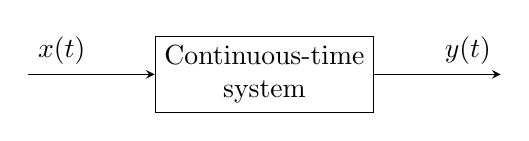
\begin{tikzpicture}
      \node[rectangle,draw,align=center](box1) at (0,0) {Continuous-time\\system};
      \begin{scope}[->,>=stealth]
        \draw (-3,0) node[above right] {$x(t)$} -- (box1);
        \draw (box1) -- (3,0) node[above left] {$y(t)$};
      \end{scope}
    \end{tikzpicture}
    }\hspace{1em}
    \subfigure[离散时间系统]{
    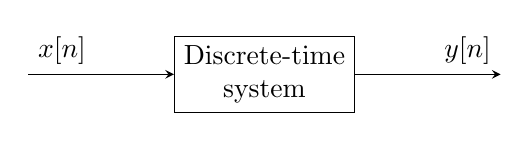
\begin{tikzpicture}
      \node[rectangle,draw,align=center](box2) at (0,0) {Discrete-time\\system};
      \begin{scope}[->,>=stealth]
        \draw (-3,0) node[above right] {$x[n]$} -- (box2);
        \draw (box2) -- (3,0) node[above left] {$y[n]$};
      \end{scope}
    \end{tikzpicture}
    }
    \caption{系统的具象}
  \end{figure}
\end{definition}
本章主要的讨论对象是\colorbox{yellow!20}{线性动态系统}(LDS),其中就包括
\[
    \begin{cases}
      \text{连续时间,线性动态系统}:CT\ LDS\\
      \text{离散时间,线性动态系统}:DT\ LDS
    \end{cases}
\]我们通过下面的几例来强化“系统”的概念.
\begin{example}
  设一个质量为$m$的长方体被弹簧吊着,从平衡状态开始,在空气中作垂直方向的振动,
  用$y(t)$表示质点在时刻$t$的位置,质点在运动中受到的力有:弹簧的恢复力$F_k$、
  阻尼器阻力$F_V(t)$和外力$F(t)$.弹簧的恢复力$F_k$与位移成正比,方向与位移相反,
  大小为$-Ky(t)$($K>0$为常数);阻尼器阻力$F_V(t)$与速度成正比,方向相反,大小为
  $-f\dot{y}(t)$($f>0$为常数).试建立弹簧阻尼系统的运动方程.
\end{example}
\begin{figure}[H]
  \centering
  \begin{tikzpicture}[>=stealth]
    \tikzstyle{spring} = [thick,decorate,decoration={aspect=0.5, segment length=1.5mm, amplitude=2mm,coil}]
    \coordinate[label=left:{$O$}] (O) at (0,0);
    \draw (O) -- (8,0);
    \draw[->] (O) -- (0,-6) node[left] {$y$};
    \foreach \i in {3,3.2,...,5}
    {
      \draw (\i,0) -- ({\i+.2},.2);
    }
    \draw[spring] (4,0) -- (4,-1);
    \draw (4,-1) -- (4,-2);
    \draw[fill=gray!20] (3,-2) rectangle (5,-3);
    \node at (4,-2.5) {$m$};
    \begin{scope}[->,>=stealth,thick]
      \draw (1,-1)node[above] {外力$F$} -| (3.5,-2);
      \draw (4.5,-2)node[right=1cm] {弹性系数$K$} -- (4.5,-1) node[right] {弹簧力$F_k$};
      \draw (4.7,-4.25) -- (4.7,-3.5) node[right] {阻尼器阻力$F_V$};
    \end{scope}
    \draw (4,-3) -- (4,-4.5);
    \draw (4,-5) -- (4,-6);
    \draw (2.7,-6) -- (5.3,-6);
    \foreach \i in {3,3.2,...,5}
    {
      \draw (\i,-6) -- ({\i-.2},-6.2);
    }
    \draw (3.5,-4) |- (2.9,-4.25) -- (2.9,-5) -- (5.1,-5) |- (4.5,-4.25) -- (4.5,-4);
    \draw[fill=gray] (2.9,-4.75) rectangle (5.1,-4.5);
    \node[right] at (5.1,-4.5) {弹性系数$f$};
  \end{tikzpicture}
  \caption{弹簧阻尼系统}
\end{figure}
\begin{solution}
  由牛顿第二定律得到弹簧的运动方程
  \begin{equation}
    \frac{-K}{m}y(t)-\frac{f}{m}\dot{y}(t)+\frac{1}{m}F(t)=\ddot{y}(t)
  \end{equation}
  \textcolor{magenta}{\HandRight}小球还可能受到其他未知的作用力,在方程中表达为随机变量$e(t)$,即
  \begin{equation}\label{eq:Motion-equation-with-random}
    \frac{-K}{m}y(t)-\frac{f}{m}\dot{y}(t)+\frac{1}{m}F(t)+e(t)=\ddot{y}(t)
  \end{equation}
  式\eqref{eq:Motion-equation-with-random}是一个\uwave{二阶线性(非齐次)微分方程},它描述了
  图示的弹簧阻尼系统的运动规律.
\end{solution}
下面我们将这个\textcolor{magenta}{二阶}方程转换为\textcolor{blue}{一阶}线性微分方程:记
\[
    \bm{X}(t)=[X_1(t),X_2(t)]^\mT=[y(t),\dot{y}(t)]^\mT
\]
那么式\eqref{eq:Motion-equation-with-random}转化为方程组
\begin{equation}
  \begin{dcases}
    \dot{X}_1(t)=X_2(t)\\
    \dot{X}_2(t)=-\frac{K}{m}X_1(t)-\frac{f}{m}X_2(t)+\frac{1}{m}F(t)+e(t)
  \end{dcases}
\end{equation}
写成矩阵形式,有
\begin{equation}
  \frac{\mathrm{d}}{\mathrm{d}t}\begin{bmatrix}
    X_1(t)\\
    X_2(t)
  \end{bmatrix}=
  \begin{bmatrix}
    0&1\\
    -\frac{K}{m}&-\frac{f}{m}
  \end{bmatrix}
  \begin{bmatrix}
    X_1(t)\\
    X_2(t)
  \end{bmatrix}+
  \begin{bmatrix}
    0\\
    \frac{1}{m}
  \end{bmatrix}F(t)+
  \begin{bmatrix}
    0\\1
  \end{bmatrix}e(t)
\end{equation}
这样我们将一个二阶线性微分方程转化成了两个一阶线性微分方程,并且写成了矩阵形式!

对于$n$阶的情况,我们需要设$n$个状态变量,将$n$阶线性微分方程转化为$n$个一阶线性微分方程.
\begin{proposition}[连续线性系统的微分方程组]\label{pro:continuous-linear-system-ODE}
  关于连续线性系统的一个$n$阶线性微分方程可以转化为$n$个一阶线性方程组成的线性方程组:
  \begin{equation}\label{eq:continuous-linear-system-ODE}
    \underset{n\times 1}{\dot{\bm{X}}}(t)=\underset{n\times n}{\bm{A}}(t)\underset{n\times 1}{\bm{X}}(t)+\underset{n\times p}{\bm{B}}(t)\underset{p\times 1}{\bm{u}}(t)+\underset{n\times q}{\bm{C}}(t)\underset{q\times 1}{\bm{e}}(t)
  \end{equation}
  其中有控制输入向量
  \[
      \bm{u}(t)=\begin{bmatrix}
        u_1(t)&u_2(t)&\cdots&u_p(t)
      \end{bmatrix}^\mT
  \]
  随机部分
  \[
      \bm{e}(t)=\begin{bmatrix}
        e_1(t)&e_2(t)&\cdots&e_q(t)
      \end{bmatrix}^\mT
  \]
  且有
  \begin{itemize}
    \item $E[\bm{e}(t)]=0$;
    \item $\Cov[\bm{e}(t),\bm{e}(\tau)]=\bm{D}_e(t)\delta(t-\tau)$.
  \end{itemize}
\end{proposition}
\begin{note}
    需要注意的是:此处系统的随机部分和观测方程
    \[
        \bm{Z}(t)=\bm{F}[\bm{X}(t)]+\bm{\varDelta}(t)
    \]
    中的观测误差$\bm{\varDelta}(t)$不是一个概念,且总是无关的,即
    \begin{equation}
      \Cov[\bm{\varDelta}(t),\bm{e}(\tau)]=0.
    \end{equation}
  \end{note}
对于连续\uwave{时不变}系统,各项系数与时间无关,故状态方程退化为
\begin{equation}
  \dot{\bm{X}}(t)=\bm{A}\bm{X}(t)+\bm{B}\bm{u}(t)+\bm{C}\bm{e}(t)
\end{equation}
若不考虑系统的输入,那么有无输入的状态方程
\begin{equation}
  \dot{\bm{X}}(t)=\bm{A}(t)\bm{X}(t)+\bm{C}(t)\bm{e}(t)
\end{equation}

更多时候我们考虑非线性系统,下面我们就\uline{连续非线性系统的线性化}这个命题进行讨论.

给出非线性系统的微分方程组:
\begin{equation}
  \dot{\bm{X}}(t)=\bm{g}[\bm{X}(t),\bm{u}(t),\bm{e}(t)]
\end{equation}
其中$\bm{g}$是关于$\bm{X}$,\ $\bm{u}$,\ $\bm{e}$的三元非线性函数.
\begin{note}
  $\bm{u}(t)$并不是随机量!其具体意义是\textcolor{magenta}{外界的输入},只是
  我们在列立方程时必须要考虑该元素.
\end{note}
由于$\bm{u}$并不是随机量,也就是说函数$\bm{g}$的真正自变量只有下面标红的两个:
\[
  \dot{\bm{X}}(t)=\bm{g}[\textcolor{magenta}{\bm{X}(t)},\bm{u}(t),\textcolor{magenta}{\bm{e}(t)}]
\]
下面给出结论
\begin{proposition}[连续非线性系统的线性化]\label{pro:linearization-of-nonlinear-system}
  对于描述连续非线性系统的状态方程
  \[
    \dot{\bm{X}}(t)=\bm{g}[\bm{X}(t),\bm{u}(t),\bm{e}(t)]
  \]
  对其进行线性化得到下式
  \begin{equation}
    \dot{\bm{X}}(t)=\bm{A}(t)\bm{X}(t)+\bm{g}[\bm{X}^*(t),\bm{u}(t),0]-\bm{A}(t)\bm{X}^*(t)+\bm{C}(t)\bm{e}(t)
  \end{equation}
  其中$\bm{A}(t)$和$\bm{C}(t)$分别是自变量$\bm{X}(t)$和$\bm{e}(t)$的\textup{Jacobi}矩阵.
\end{proposition}
通常记
\[
    \bm{G}:=\bm{g}[\bm{X}^*(t),\bm{u}(t),0]-\bm{A}(t)\bm{X}^*(t)
\]
则
\[
  \dot{\bm{X}}(t)=\bm{A}(t)\bm{X}(t)+\bm{G}(t)+\bm{C}(t)\bm{e}(t)
\]  
\begin{example}
  卫星的轨迹可以用$r(t)$和$\theta(t)$两个极坐标变量表示.其中$r(t)$是卫星
  到地面的距离,\ $\theta(t)$是卫星和地心的连线相对于参考坐标轴的角度.假定
  卫星具有在轨道径向和切向的推力控制$u_r(t)$和$u_l(t)$,试建立卫星轨迹控制系统
  的模型并进行线性化.
\end{example}
\begin{solution}
  根据受力分析:
  \begin{equation}\label{eq:important-example-2.1}
    \ddot{r}(t)=r(t)[\dot{\theta}(t)]^2-\frac{GM}{r^2(t)}+u_r(t)+e_r(t)
  \end{equation}
  \begin{equation}\label{eq:important-example-2.2}
    \ddot{\theta}(t)=-\frac{2}{r(t)}\dot{\theta}(t)\dot{r}(t)+\frac{1}{r(t)}u_l(t)+e_{\theta}(t)
  \end{equation}
  设状态变量为
  \[
      \bm{X}(t)=\begin{bmatrix}
        X_1(t)\\
        X_2(t)\\
        X_3(t)\\
        X_4(t)
      \end{bmatrix}=
      \begin{bmatrix}
        r(t)\\
        \dot{r}(t)\\
        \theta(t)\\
        \dot{\theta}(t)
      \end{bmatrix}
  \]
  将方程\eqref{eq:important-example-2.1}和\eqref{eq:important-example-2.2}整理成矩阵形式,有
  \begin{equation}\label{eq:important-example-2.3}
    \begin{bmatrix}
      \dot{X}_1(t)\\
      \dot{X}_2(t)\\
      \dot{X}_3(t)\\
      \dot{X}_4(t)
    \end{bmatrix}=
    \begin{bmatrix}
      X_2(t)\\
      X_1(t)X_4^2(t)-\frac{GM}{X_1^2(t)}+u_r(t)\\
      X_4(t)\\
      -\frac{2}{X_1(t)}X_4(t)X_2(t)+\frac{1}{X_1(t)}u_l(t)
    \end{bmatrix}+
    \begin{bmatrix}
      0&0\\
      1&0\\
      0&0\\
      0&1
    \end{bmatrix}
    \begin{bmatrix}
      e_r(t)\\
      e_\theta(t)
    \end{bmatrix}
  \end{equation}
  记式\eqref{eq:important-example-2.3}中最大的矩阵为
  \[
      \begin{bmatrix}
        g_1(\bm{X}(t),\bm{u}(t))\\
        g_2(\bm{X}(t),\bm{u}(t))\\
        g_3(\bm{X}(t),\bm{u}(t))\\
        g_4(\bm{X}(t),\bm{u}(t))
      \end{bmatrix}
  \]
  几个比较难处理的一阶偏导数:
  \[
      \frac{\partial g_2}{\partial X_1}=[X_4^*(t)]^2+\frac{2GM}{[X_1^*(t)]^3},\qquad\frac{\partial g_2}{\partial X_4}=2X_1^*(t)X_4^*(t)
  \]
  \[
      \frac{\partial g_4}{\partial X_1}=\frac{2X_2^*(t)X_4^*(t)}{[X_1^*(t)]^2}-\frac{u_l(t)}{[X_1^*(t)]^2},\qquad\frac{\partial g_4}{\partial X_2}=-\frac{2X_4^*(t)}{X_1^*(t)},\qquad\frac{\partial g_4}{\partial X_4}=-\frac{2X_2^*(t)}{X_1^*(t)}
  \]
  那么我们就能得到
  \[
      \bm{A}=\begin{bmatrix}
        0&1&0&0\\
        \partial g_2/\partial X_1&0&0&\partial g_2/\partial X_4\\
        0&0&0&1\\
        \partial g_4/\partial X_1&\partial g_4/\partial X_2&0&\partial g_4/\partial X_4
      \end{bmatrix}
  \]
  \[
    \bm{C}=\begin{bmatrix}
      0&0\\
      1&0\\
      0&0\\
      0&1
    \end{bmatrix}
  \]  
  也就不难写出线性化的最终形式.
\end{solution}
\section{状态转移矩阵和连续性线性系统的解}
下面我们的任务就是要求解微分方程,常用的解法有
\[
    \begin{cases}
      \text{解析法求解}\\
      \text{数值积分法}
    \end{cases}
\]
我们简单回顾一下用解析法处理一阶线性非齐次微分方程的步骤:
\begin{theorem}[一阶线性非齐次微分方程处理办法]\label{thm:1-order-non-homogeneous-linear-DE}
  形如
  \begin{equation}
    \dot{y}+P(x)y=Q(x)
  \end{equation}
  的微分方程式是\uwave{一阶,非齐次,线性,微分方程}.\\
  \textbf{Step\ 1}\ 求得对应齐次方程
  \[
      \dot{y}+P(x)y=0
  \]
  的解
  \begin{equation}
    y=Ce^{-\int \!P(x)\md x}
  \end{equation}
  \textbf{Step\ 2}\ 考虑常数变易法,待定函数$C(x)$,将
  \[
      y=C(x)e^{-\int \!P(x)\md x}
  \]
  代入原方程,求得
  \begin{equation}
    C(x)=\int Q(x)e^{\int \!P(x)\md x}+C
  \end{equation}
  \textbf{Step\ 3}\ 得到方程的通解
  \begin{equation}
    y=Ce^{-\int \!P(x)\md x}+e^{-\int \!P(x)\md x}\int Q(x)e^{\int \!P(x)\md x}
  \end{equation}
\end{theorem}
\subsection{齐次解}
根据定理\ref{thm:1-order-non-homogeneous-linear-DE}中所描述的方法,我们
先考虑方程\eqref{eq:continuous-linear-system-ODE}:
\[
    \dot{\bm{X}}(t)=\bm{A}(t)\bm{X}(t)+\bm{B}(t)\bm{u}(t)+\bm{C}(t)\bm{e}(t)
\]
对应齐次方程:
\begin{equation}\label{eq:homogeneous-equation}
    \dot{\bm{X}}(t)-\bm{A}(t)\bm{X}(t)=0
\end{equation}
的解——这是最简单的一阶线性齐次微分方程,容易解得
\begin{equation}\label{eq:homogeneous-solution}
  \bm{X}(t)=\exp\left\{\int_{t_0}^t\bm{A}(\tau)\md\tau\right\}\bm{X}(t_0)
\end{equation}

研究上式\eqref{eq:homogeneous-solution}发现,因子$\exp\{\int_{t_0}^t\bm{A}(\tau)\md\tau\}$把
$t_0$时的初始状态转移到了$t$时刻的状态,所以我们记
\begin{equation}\label{eq:state-trans-matrix}
  \bm{\varPhi}(t,t_0):=\exp\left\{\int_{t_0}^t\bm{A}(\tau)\md\tau\right\}
\end{equation}
称之为\CJKunderdot{状态转移矩阵}.
\begin{property}状态转移矩阵的性质:
  \begin{enumerate}
    \item $\dot{\bm{\varPhi}}(t,t_0)=\bm{A}(t)\bm{\varPhi}(t,t_0)$;
    \item $\bm{\varPhi}(t_0,t_0)=\bm{I}$;
    \item 分段转移:\ $\bm{\varPhi}(t_2,t_0)=\bm{\varPhi}(t_2,t_1)\bm{\varPhi}(t_1,t_0)$;
    \item 转移可逆:\ $\bm{\varPhi}(t,t_0)=\bm{\varPhi}^{-1}(t_0,t)$.
  \end{enumerate}
\end{property}
选取证明性质1
\begin{proof}
  将$\bm{X}(t)=\bm{\varPhi(t,t_0)}\bm{X}(t_0)$代回原方程\eqref{eq:homogeneous-equation}
  就能得到该性质.
  
  或者直接对状态转移矩阵求导:
  \[
      \frac{\mathrm{d}}{\mathrm{d}t}\bm{\varPhi}(t,t_0)=\left(\int_{t_0}^t\bm{A}(\tau)\md\tau\right)'\exp\left\{\int_{t_0}^t\bm{A}(\tau)\md\tau\right\}
  \]
  依据变限积分求导法则\ref{thm:uncertained-limited-integral}就能得到结果.
\end{proof}
对于线性时不变系统,得解
\begin{equation}\label{eq:homogeneous-solution-for-nontime-system}
  \bm{X}(t)=\exp\left\{\bm{A}\times(t-t_0)\right\}\bm{X}_0
\end{equation}
此时状态转移矩阵
\begin{equation}\label{eq:state-trans-matrix-for-nontime-system}
  \bm{\varPhi}(t,t_0)=\bm{\varPhi}(\Delta t)=\exp\{\bm{A}\times\Delta t\}
\end{equation}
\begin{property}时不变系统转移矩阵的性质\\
  $\bm{\varPhi}(k\cdot\Delta t)=e^{\bm{A}\cdot k\Delta t}=\underbrace{e^{\bm{A}\Delta t}\cdot e^{\bm{A}\Delta t}\cdots e^{\bm{A}\Delta t}}_{k\text{个}}=[\bm{\varPhi}(\Delta t)]^k$.
\end{property}
来到一个有关\emph{矩阵的指数}的有意思话题,我们该怎样计算一个矩阵的指数$e^{\bm{A}}$\ ?

答案是对于方阵$\bm{A}$,可以通过\textup{Taylor}展开的方式来计算矩阵指数,即对于“矩阵幂级数”
\begin{equation}
  e^{\bm{x}}=\bm{I}+\bm{x}+\frac{1}{2!}\bm{x}^2+\cdots+\frac{1}{k!}\bm{x}^k+\cdots
\end{equation}
将$\bm{x}=\bm{A}$即可得解.
\begin{example}\label{ex:nontime-system}
  已知系统的状态方程为
  \[
    \dot{\bm{X}}=\begin{bmatrix}
      0&1\\
      0&0
    \end{bmatrix}\bm{X},
  \]  
  初始条件为$\bm{X}(0)$,试求状态转移矩阵和状态方程的解.
\end{example}
\begin{solution}
  这显然是一个线性时不变系统,因为矩阵系数$\bm{A}$与时间变量$t$没有关系.且状态方程是一个
  一阶线性齐次微分方程,根据式\eqref{eq:homogeneous-solution-for-nontime-system}和式\eqref{eq:state-trans-matrix-for-nontime-system}
  可以得到此时
  \begin{equation}\label{eq:State-Trans-Matrix-Taylor-expansion}
    \bm{\varPhi}(t)=e^{\bm{A}t}=\bm{I}+\bm{A}t+\frac{1}{2!}\bm{A}^2t^2+\cdots+\frac{1}{k!}\bm{A}^kt^k+\cdots
  \end{equation}
  \[
      \bm{X}(t)=\bm{\varPhi}(t)\bm{X}(0)
  \]
  因为
  \[
      \bm{A}=\begin{bmatrix}
        0&1\\
        0&0
      \end{bmatrix},\quad
      \bm{A}^2=\bm{A}^3=\cdots=\bm{A}^k=\begin{bmatrix}
        0&0\\
        0&0
      \end{bmatrix}
  \]
  所以状态转移矩阵
  \[
      \bm{\varPhi}(t)=\begin{bmatrix}
        1&t\\
        0&1
      \end{bmatrix}
  \]
  \textcolor{magenta}{\HandRight}关于状态转移矩阵的这个结论非常常用,请务必记住!

  状态方程的解
  \[
      \bm{X}(t)=\begin{bmatrix}
        1&t\\
        0&1
      \end{bmatrix}\bm{X}(0)
  \]
  由物理意义来理解此题,有状态变量
  \[
      \bm{X}=\begin{bmatrix}
        r(t)\\
        v(t)
      \end{bmatrix},\quad\dot{\bm{X}}=\begin{bmatrix}
        v(t)\\
        a(t)
      \end{bmatrix}
  \]
  那么解被诠释为
  \[
      \begin{cases}
        r(t)=r_0+v_0t,\\
        v(t)=v_0,
      \end{cases}
  \]
  这是一个\uline{匀速直线运动过程}.
\end{solution}
\begin{example}
  将题目\ref{ex:nontime-system}推广至$n$维情况,即
  \[
      \dot{\bm{X}}=\begin{bmatrix}
        0&1&0&\cdots&0\\
        0&0&1&\cdots&0\\
        \vdots&\vdots&\vdots&\ddots&\vdots\\
        0&0&0&\cdots&1\\
        0&0&0&\cdots&0
      \end{bmatrix}\bm{X}(0)
  \]
  求此时的状态转移矩阵和状态方程解.
\end{example}
\begin{solution}
  根据归纳,
  \[
      \underset{n\times n}{\bm{A}^k}=\begin{bmatrix}
        \underset{(n-k)\times k}{\bm{O}}&\underset{(n-k)\times(n-k)}{\bm{I}}\\
        \underset{k\times k}{\bm{O}}&\underset{k\times(n-k)}{\bm{O}}
      \end{bmatrix}
  \]
  也就是说当$n\geqslant k$时,\ $\bm{A}$矩阵就成了零矩阵,也即\textup{Taylor}展开
  在$n\geqslant k$后的项都是零矩阵.

  不难得到
  \[
      \underset{n\times n}{\bm{\varPhi}}(t)=\begin{bmatrix}
        1&t&t^2/2&t^3/6&\cdots&t^{n-1}/(n-1)!\\
        0&1&t&t^2/2&\cdots&t^{n-2}/(n-2)!\\
        0&0&1&t&\cdots&t^{n-3}/(n-3)!\\
        0&0&0&1&\cdots&t^{n-4}/(n-4)!\\
        \vdots&\vdots&\vdots&\vdots&\ddots&\vdots\\
        0&0&0&0&\cdots&1
      \end{bmatrix}
  \]
  以及状态方程的解.
\end{solution}
\subsection{非齐次解}
下面考虑非齐次方程:
\[
    \dot{\bm{X}}(t)=\bm{A}(t)\bm{X}(t)+\bm{B}(t)\bm{u}(t)+\bm{C}(t)\bm{e}(t)
\]
我们已经有齐次方程的解\eqref{eq:homogeneous-solution}:
\begin{align*}
  \bm{X}(t)&=\exp\left\{\int_{t_0}^t\bm{A}(\tau)\md\tau\right\}\bm{X}(t_0)\\
  &=\bm{\varPhi}(t,t_0)\bm{X}(t_0)
\end{align*}
  
考虑\colorbox{yellow!20}{常数变易法},令$\bm{X}(t_0)\to \bm{\xi}(t)$,有
\begin{equation}\label{eq:constant-simply}
  \bm{X}(t)=\bm{\varPhi}(t,t_0)\bm{\xi}(t)
\end{equation}
将其代回原方程,因为
\begin{equation}
  \dot{\bm{X}}(t)=\bm{\varPhi}(t,t_0)\dot{\bm{\xi}}(t)+\dot{\bm{\varPhi}}(t,t_0)\bm{\xi}(t)
\end{equation}
所以状态转移矩阵的性质1和性质4,代入整理得
\begin{align*}
  \bm{\varPhi}(t,t_0)\dot{\bm{\xi}}(t)+\bm{A}(t)\bm{\varPhi}(t,t_0)\bm{\xi}(t)&=\bm{A}(t)\bm{\varPhi}(t,t_0)\bm{\xi}(t)+\bm{B}(t)\bm{u}(t)+\bm{C}(t)\bm{e}(t)\\
  \dot{\bm{\xi}}(t)&=\bm{\varPhi}^{-1}(t,t_0)\bm{B}(t)\bm{u}(t)+\bm{\varPhi}^{-1}(t,t_0)\bm{C}(t)\bm{e}(t)\\
  \dot{\bm{\xi}}(t)&=\bm{\varPhi}(t_0,t)\bm{B}(t)\bm{u}(t)+\bm{\varPhi}(t_0,t)\bm{C}(t)\bm{e}(t)
\end{align*}
对上式求积分,有
\begin{equation}
  \bm{\xi}(t)-\bm{\xi}(t_0)=\int_{t_0}^t\bm{\varPhi}(t_0,\tau)\bm{B}(\tau)\bm{u}(\tau)\md\tau+\int_{t_0}^t\bm{\varPhi}(t_0,\tau)\bm{C}(\tau)\bm{e}(\tau)\md\tau
\end{equation}
其中初值$\bm{\xi}(t_0)$可以由$t=t_0$代入式\eqref{eq:constant-simply}得到:
\begin{equation}
  \bm{\xi}(t_0)=\bm{X}(t_0)
\end{equation}
综合\uline{得解非齐次方程的解}:
\begin{equation}
  \boxed{
  \bm{X}(t)=\bm{\varPhi}(t,t_0)\bm{X}(t_0)+\int_{t_0}^t\bm{\varPhi}(t,\tau)\bm{B}(\tau)\bm{u}(\tau)\md\tau+\int_{t_0}^t\bm{\varPhi}(t,\tau)\bm{C}(\tau)\bm{e}(\tau)\md\tau
  }
\end{equation}
\section{离散线性系统的数学模型}
既得连续线性系统状态方程的解
\begin{theorem}[连续线性系统状态方程的解]\label{thm:continuous-linear-system-solution}
  对于一个连续线性系统的状态方程
  \[
      \dot{\bm{X}}(t)=\bm{A}(t)\bm{X}(t)+\bm{B}(t)\bm{u}(t)+\bm{C}(t)\bm{e}(t),
  \]
  它的解是
  \[
      \bm{X}(t)=\underbrace{\bm{\varPhi}(t,t_0)\bm{X}(t_0)}_{\text{齐次解}}+\int_{t_0}^t\bm{\varPhi}(t,\tau)\bm{B}(\tau)\bm{u}(\tau)\md\tau+\int_{t_0}^t\bm{\varPhi}(t,\tau)\bm{C}(\tau)\bm{e}(\tau)\md\tau.
  \]
  其中
  \[
    E[\bm{e}(t)]=0,
  \]  
  \[
      \Cov[\bm{e}(t),\bm{e}(\tau)]=\bm{D}_e(t)\delta(t-\tau).
  \]
\end{theorem}
在实际应用中,我们必须指出
\begin{note}
  \begin{itemize}
    \item 离散情况比连续情况更多见!
    \item 数值解法比解析解法更通用!
  \end{itemize}
\end{note}
就拿上面的非齐次解来说,第二、三项的积分往往因为用不了Newton-Leibniz公式(被积函数不存在原函数)
而不存在解析解,我们只得考虑数值法,比如将被积函数按幂级数展开再逐项积分......

或者我们可以直接分析\textcolor{magenta}{离散系统}——考虑将积分区间$[t_0,t]$进行划分:
\[
    \textcolor{magenta}{t_0}<t_1<t_2<\cdots<t_k=\textcolor{magenta}{t}
\]
得到$k$个时间区间和$k+1$个时间点,再将非齐次解的形式改到这$k$个区间里:
\begin{equation}\label{eq:discrete-system-equation}
  \bm{X}(t_k)=\bm{\varPhi}(t_k,t_{k-1})\bm{X}(t_{k-1})+\underbrace{\int_{t_{k-1}}^{t_k}\bm{\varPhi}(t_k,\tau)\bm{B}(\tau)\bm{u}(\tau)\md\tau}_{=:\underset{n\times 1}{\bm{\Omega}}(k-1)}+\underbrace{\int_{t_{k-1}}^{t_k}\bm{\varPhi}(t_k,\tau)\bm{C}(\tau)\bm{e}(\tau)\md\tau}_{=:\underset{n\times 1}{\bm{w}}(k-1)}
\end{equation}
\[
  \bm{X}(t_{k-1})=\bm{\varPhi}(t_{k-1},t_{k-2})\bm{X}(t_{k-2})+\int_{t_{k-2}}^{t_{k-1}}\bm{\varPhi}(t_{k-1},\tau)\bm{B}(\tau)\bm{u}(\tau)\md\tau+\int_{t_{k-2}}^{t_{k-1}}\bm{\varPhi}(t_{k-1},\tau)\bm{C}(\tau)\bm{e}(\tau)\md\tau
\]
\[
    \vdots
\]
\[
  \bm{X}(t_1)=\bm{\varPhi}(t_1,t_0)\bm{X}(t_0)+\int_{t_0}^{t_1}\bm{\varPhi}(t_1,\tau)\bm{B}(\tau)\bm{u}(\tau)\md\tau+\int_{t_0}^{t_1}\bm{C}(\tau)\bm{e}(\tau)\md\tau
\]
考虑式\eqref{eq:discrete-system-equation}的记法,此外另记
\[
    \bm{X}(t_k)\longrightarrow\bm{X}(k)
\]
\[
    \bm{\varPhi}(t_k,t_{k-1})\longrightarrow\bm{\varPhi}_{k,k-1}
\]
我们就能得到一组\CJKunderdot{差分方程}:
\begin{equation}\label{eq:discrete-system-equation-easy}
  \boxed{\bm{X}(k)=\bm{\varPhi}_{k,k-1}\bm{X}(k-1)+\bm{\Omega}(k-1)+\bm{w}(k-1)}
\end{equation}
\[
  \bm{X}(k-1)=\bm{\varPhi}_{k-1,k-2}\bm{X}(k-2)+\bm{\Omega}(k-2)+\bm{w}(k-2)
\]
\[
    \vdots
\]
\[
  \bm{X}(1)=\bm{\varPhi}_{1,0}\bm{X}(0)+\bm{\Omega}(1)+\bm{w}(1)
\]
若初值$\bm{X}(0)$已知,就可以依次推导出$\bm{X}(1)$,\ $\bm{X}(2)$,\ $\cdots$,\ $\bm{X}(k)$,最后得到
\begin{equation}
  \bm{X}(k)=\bm{\varPhi}_{k,0}\bm{X}(0)+\sum_{i=1}^k\bm{\varPhi}_{k,i}\bm{\Omega}(i-1)+\sum_{i=1}^k\bm{\varPhi}_{k,i}\bm{w}(i-1)
\end{equation}

当时间的划分使得$\Delta t\to 0$时,我们还可以记第二项\footnote{实际上笔者并不知道为什么书中可以采取这样的记法,或许是出于线性化,
或许是处于离散化,或许是考虑了中值定理}
\[
  \int_{t_{k-1}}^{t_k}\bm{\varPhi}(t_k,\tau)\bm{B}(\tau)\bm{u}(\tau)\md\tau\longrightarrow\bm{\varPsi}_{k,k-1}\bm{u}(k-1)
\]
对观测方程也可以进行离散化:
\begin{equation}
  \bm{z}(k)=\bm{H}(k)\bm{X}(k)+\bm{\varDelta}(k)
\end{equation}
其中
\begin{equation}
  \bm{z}(k)=\bm{Z}(k)-\bm{F}[\bm{X}^*(k)]+\bm{H}_k\bm{X}^*(k)
\end{equation}

对于非控制科学与工程的学生,我们往往对解的第二项不感兴趣,在我们导航工程领域的大多数情况下它也很识趣地等于为零\footnote{在小节\ref{ssec:system-more}中我们认识到这样的系统是独立的(autonomous)}.令我们好奇的
是第三项,作为有关高斯白噪声的一个积分,它是否还具有高斯白噪声的性质.

我们直接不加证明地给出结论好了:
\begin{conclusion}离散线性系统的随机模型
  \begin{enumerate}
    \item $\displaystyle E[\bm{w}(k-1)]=0$;
    \item $\displaystyle \bm{D}_w(k-1)=\int_{t_{k-1}}^{t_k}\bm{\varPhi}(t_k,\tau)\bm{C}(\tau)\bm{D}_e(\tau)\bm{C}^\mT(\tau)\bm{\varPhi}^\mT(t_k,\tau)\md\tau$;
    \item $\Cov[\bm{w}(k),\bm{w}(j)]=\bm{D}_w(k)\delta_{kj},\quad\delta_{kj}$是\textup{Kronecker} $\delta$函数.
  \end{enumerate}
\end{conclusion}
\textcolor{magenta}{\HandRight}有关方差阵的差分方程组:
\begin{equation}
  \bm{D}_X(k)=\bm{\varPhi}_{k,k-1}\bm{D}_X(k-1)\bm{\varPhi}^\mT_{k,k-1}+\bm{D}_w(k-1)
\end{equation}
\[
  \bm{D}_X(k-1)=\bm{\varPhi}_{k-1,k-2}\bm{D}_X(k-2)\bm{\varPhi}^\mT_{k-1,k-2}+\bm{D}_w(k-2)
\]
\[
    \vdots
\]
\[
  \bm{D}_X(1)=\bm{\varPhi}_{1,0}\bm{D}_X(0)\bm{\varPhi}^\mT_{1,0}+\bm{D}_w(0)
\]
所以最终得到
\begin{equation}
  \bm{D}_X(k)=\bm{\varPhi}_{k,0}\bm{D}_X(0)\bm{\varPhi}^\mT_{k,0}+\sum_{i=1}^k\bm{\varPhi}(k,i)\bm{D}_w(i-1)\bm{\varPhi}_{k,i}^\mT.
\end{equation}
\begin{example}
  已知系统的状态方程为
  \begin{equation}
    \begin{bmatrix}
      \dot{x}_1(t)\\
      \dot{x}_2(t)
    \end{bmatrix}=\begin{bmatrix}
      0&1\\
      0&0
    \end{bmatrix}\begin{bmatrix}
      x_1(t)\\
      x_2(t)
    \end{bmatrix}+\begin{bmatrix}
      0\\
      1
    \end{bmatrix}e(t)
  \end{equation}
  系统噪声$e(t)$为白噪声过程,\ $q^2$为
  $e(t)$的均方值,求离散化的状态方程和它的随机模型.
\end{example}
\begin{solution}
  一些显而易见的东西:
  \[
      \bm{A}=\begin{bmatrix}
        0&1\\
        0&0
      \end{bmatrix},\quad\bm{C}=\begin{bmatrix}
        0\\
        1
      \end{bmatrix},\quad\bm{\varPhi}(t_k,\tau)=\begin{bmatrix}
        1&t_k-\tau\\
        0&1
      \end{bmatrix}
  \]
  列出离散线性系统的差分方程,即状态方程
  \[
      \bm{X}(k)=\begin{bmatrix}
        1&t_k-t_{k-1}\\
        0&1
      \end{bmatrix}\bm{X}(k-1)+\bm{w}(k-1),\quad\bm{w}(k-1)=\int_{t_{k-1}}^{t_k}\bm{\varPhi}(t_k,\tau)\bm{C}(\tau)\bm{e}(\tau)\md\tau
  \]
  随机模型
  \begin{align*}
    \bm{D}_w(k-1)&=\int_{t_{k-1}}^{t_k}\bm{\varPhi}(t_k,\tau)\bm{C}(\tau)\bm{D}_e(\tau)\bm{C}^\mT(\tau)\bm{\varPhi}^\mT(t_k,\tau)\md\tau\\
    &=\int_{t_{k-1}}^{t_k}\begin{bmatrix}
      1&t_k-\tau\\
      0&1
    \end{bmatrix}\begin{bmatrix}
      0\\
      1
    \end{bmatrix}
    q^2
    \begin{bmatrix}
      0&1
    \end{bmatrix}
    \begin{bmatrix}
      1&0\\
      t_k-\tau&1
    \end{bmatrix}\md\tau\\
    &=\int_{t_{k-1}}^{t_k}q^2\begin{bmatrix}
      (t_k-\tau)^2&t_k-\tau\\
      t_k-\tau&1
    \end{bmatrix}\md\tau
  \end{align*}
  根据矩阵的求导规则\ref{def:Matrix-Differential-and-Integrate},容易得到最后的方差阵
  \begin{equation}
    \bm{D}_w(k-1)=q^2\begin{bmatrix}
      \frac{\Delta t^3}{3}&\frac{\Delta t^2}{2}\\
      \frac{\Delta t^2}{2}&\Delta t
    \end{bmatrix},\quad\Delta t=t_k-t_{k-1}.
  \end{equation}
\end{solution}
根据上题可以归纳处下面的表格
\begin{table}[H]
  \caption{连续动态系统和离散化的动态系统}
  \begin{center}
  \begin{tabular}{ccc|cc}
  \toprule[2pt]
  \multicolumn{3}{c|}{连续动态系统} &
    \multicolumn{2}{c}{离散动态系统($\Delta t=t_k-t_{k-1}$)} \\ \hline
  \multicolumn{3}{c|}{$\dot{\bm{X}}(t)=\bm{A}(t)\bm{X}(t)+\bm{B}(t)\bm{u}(t)+\bm{C}(t)\bm{e}(t)$} &
    \multicolumn{2}{c}{$\bm{X}(k)=\bm{\varPhi}_{k,k-1}\bm{X}(k-1)+\bm{\Omega}(k-1)+\bm{w}(k-1)$} \\ \hline
  \multicolumn{1}{c|}{$\bm{A}(t)$} &
    \multicolumn{1}{c|}{$\bm{C}(t)$} &
    $\bm{D}_e(t)$ &
    \multicolumn{1}{c|}{$\bm{\varPhi}_{k,k-1}$} &
    $\bm{D}_w(k-1)$ \\ \hline
  \multicolumn{1}{c|}{$[0]$} &
    \multicolumn{1}{c|}{$[1]$} &
    $q^2$ &
    \multicolumn{1}{c|}{$[1]$} &
    $[q\Delta t]$ \\ \hline
  \multicolumn{1}{c|}{\begin{tabular}[c]{@{}c@{}}$\begin{bmatrix}0&1\\ 0&0 \end{bmatrix}$\end{tabular}} &
    \multicolumn{1}{c|}{\begin{tabular}[c]{@{}c@{}}$\begin{bmatrix}0\\ 1 \end{bmatrix}$\end{tabular}} &
    $q^2$ &
    \multicolumn{1}{c|}{\begin{tabular}[c]{@{}c@{}}$\begin{bmatrix}1&\Delta t\\ 0&1 \end{bmatrix}$\end{tabular}} &
    \begin{tabular}[c]{@{}c@{}}$q^2\begin{bmatrix}\frac{\Delta t^3}{3}&\frac{\Delta t^2}{2}\\ \frac{\Delta t^2}{2}&\Delta t \end{bmatrix}$\end{tabular} \\ \hline
  \multicolumn{1}{c|}{\begin{tabular}[c]{@{}c@{}}$\begin{bmatrix}0&1&0\\0&0&1\\0&0&0\end{bmatrix}$\end{tabular}} &
    \multicolumn{1}{c|}{\begin{tabular}[c]{@{}c@{}}$\begin{bmatrix}0\\ 0\\1\end{bmatrix}$\end{tabular}} &
    $q^2$ &
    \multicolumn{1}{c|}{\begin{tabular}[c]{@{}c@{}}$\begin{bmatrix}1&\Delta t&\frac12\Delta t^2\\ 0&1&\Delta t\\ 0&0&1 \end{bmatrix}$\end{tabular}} &
    \begin{tabular}[c]{@{}c@{}}$q^2\begin{bmatrix}\frac{\Delta t^5}{20}&\frac{\Delta t^4}{8}&\frac{\Delta t^3}{6}\\\frac{\Delta t^4}{8}&\frac{\Delta t^3}{3}&\frac{\Delta t^2}{2}\\\frac{\Delta t^3}{6}&\frac{\Delta t^2}{2}&\Delta t\end{bmatrix}$\end{tabular} \\ \bottomrule[2pt]
  \end{tabular}
  \end{center}
\end{table}
\section{随机过程的进一步讨论}\label{sec:controllability-and-measurability}
在GNSS相位观测值中,我们只能测得不足整周的波长,之前的
整周数$N$可以用\uwave{随机常数}来表示:
\[
    \dot{N}=0,
\]
\[
    \bm{D}_w(k-1)=0.
\]
钟差、钟漂可以用随机游走过程来表示:
\[
    \dot{x}(t)=e(t)
\]
卫星运动中未模型化的加速度部分可以视为
Gauss-Markov过程,我们此处重新给出其定义:
\begin{definition}[Gauss-Markov过程]\label{def:Gauss-Markov-process2}
  $x(t)$是\textup{Markov}随机过程,当其对于时间$t_1<t_2<\cdots<t_k$满足
  \begin{equation}
    P\left[x(t_k)\mid x(t_{k-1}),\ldots,x(t_1)\right]=P\left[x(t_k)\mid x(t_{k-1})\right]
  \end{equation}
  时(用语言来描述就是一种\CJKunderdot{无后效性}).

  一阶的\textup{Markov}过程满足
  \begin{equation}
    \dot{x}(t)+\beta x(t)=e(t),
  \end{equation}
  其中$e(t)$是白噪声过程.

  一阶的\textup{Gauss-Markov}过程也满足上式,只不过此时$e(t)$
  是高斯白噪声.
\end{definition}
利用一阶线性非齐次微分方程的解法定理\ref{thm:1-order-non-homogeneous-linear-DE},不难
解得Gauss-Markov过程的解
\begin{equation}
  x(t)=x(t_0)e^{-\beta(t-t_0)}+\int_{t_0}^te^{-\beta(t-t_0)}e(\tau)\md\tau
\end{equation}
将情况直接推广至离散情形,有
\begin{equation}
  x(k)=e^{-\beta(t_k-t_{k-1})}x(k-1)+w(k-1),
\end{equation}
其中
\begin{equation}
  w(k-1)=\int_{t_{k-1}}^{t_k}e^{-\beta(t_k-\tau)}e(\tau)\md\tau.
\end{equation}

例题\ref{ex:nontime-system}中系统的状态方程是一个典型的描述\uline{随机斜坡过程}的方程,参看
随机斜坡过程的定义\ref{def:random-slope-process}:
\[
    \begin{cases}
      \dot{x}_1(t)=x_2(t),\\
      \dot{x}_2(t)=0,
    \end{cases}\Longrightarrow\begin{bmatrix}
      \dot{x}_1(t)\\
      \dot{x}_2(t)
    \end{bmatrix}=\begin{bmatrix}
      0&1\\
      0&0
    \end{bmatrix}\begin{bmatrix}
      x_1(t)\\
      x_2(t)
    \end{bmatrix}\Longrightarrow\dot{\bm{X}}(t)=\begin{bmatrix}
      0&1\\
      0&0
    \end{bmatrix}\bm{X}(t)
\]
还记得我们在例题\ref{ex:nontime-system}中的相关结论吗?连续系统的解
\[
    \begin{bmatrix}
      x_1(t)\\
      x_2(t)
    \end{bmatrix}=
    \begin{bmatrix}
      1&t\\
      0&1
    \end{bmatrix}\begin{bmatrix}
      x_1(0)\\
      x_2(0)
    \end{bmatrix},
\]
离散系统的解
\[
    \begin{bmatrix}
      x_1(k)\\
      x_2(k)
    \end{bmatrix}=
    \begin{bmatrix}
      1&t_{k}-t_{k-1}\\
      0&1
    \end{bmatrix}\begin{bmatrix}
      x_1(k-1)\\
      x_2(k-1)
    \end{bmatrix},\quad \bm{D}_w(k-1)=\bm{0}.
\]
下面这道例题展现的也是随机斜坡过程.
\begin{example}
  \textup{GNSS}接收机时钟与导航系统时间频率
  不同步导致的时钟偏差$t_b$是影响\textup{GNSS}
  测距精度的主要原因,为了消除时钟偏差对定位结果的影响,
  将接收机钟差模型化并进行估计.
  
  接收机时钟频率漂移$t_d$(钟漂),是振荡器的时间
  振荡频率与标称频率之间的差异,是引起$t_b$的根本原因.

  一般将钟漂$t_d$描述为随机游走过程;钟差$t_b$认为是由钟漂
  和白噪声叠加而成的,所以钟差$t_b$的运动规律可被描述为
  \[
      \begin{bmatrix}
        \dot{t}_b(t)\\
        \dot{t}_d(t)
      \end{bmatrix}=
      \begin{bmatrix}
        0&1\\
        0&0
      \end{bmatrix}
      \begin{bmatrix}
        t_b(t)\\
        t_d(t)
      \end{bmatrix}+
      \begin{bmatrix}
        1&0\\
        0&1
      \end{bmatrix}
      \begin{bmatrix}
        e_b(t)\\
        e_d(t)
      \end{bmatrix}
  \]
  其中$e_b(t)$和$e_d(t)$均为零均值白噪声,方差阵为
  \[
      \bm{D}_e=\begin{bmatrix}
        \sigma_{e_b}^2&0\\
        0&\sigma_{e_d}^2
      \end{bmatrix}.
  \]
  求解该系统的数学模型.
\end{example}
\begin{solution}
  显然这是随机斜坡过程.状态转移矩阵
  \[
      \bm{\varPhi}(t_k,\tau)=\begin{bmatrix}
        1&t_k-\tau\\
        0&1
      \end{bmatrix}
  \]
  设$\bm{T}(t)=[t_b(t),t_d(t)]^\mT$,\ $\bm{e}(\tau)=[e_b(\tau),e_d(\tau)]^\mT$,则该离散系统的状态方程可以写作
  \[
      \bm{T}(k)=\bm{\varPhi}_{k,k-1}\bm{T}(k-1)+\int_{t_{k-1}}^{t_k}\bm{\varPhi}(t_k,\tau)\cdot\bm{C}\bm{e}(\tau)\md\tau,\quad\bm{C}=\begin{bmatrix}
        1&0\\
        0&1
      \end{bmatrix}
  \]
  系统的随机模型
  \begin{align*}
    \bm{D}_w(k-1)&=\int_{t_{k-1}}^{t_k}\bm{\varPhi}(t_k,\tau)\bm{C}(\tau)\bm{D}_e(\tau)\bm{C}^\mT(\tau)\bm{\varPhi}^\mT(t_k,\tau)\md\tau\\
    &=\int_{t_{k-1}}^{t_k}\begin{bmatrix}
      1&t_k-\tau\\
      0&1
    \end{bmatrix}
    \begin{bmatrix}
      1&0\\
      0&1
    \end{bmatrix}
    \begin{bmatrix}
      \sigma_{e_b}^2&0\\
      0&\sigma_{e_d}^2
    \end{bmatrix}
    \begin{bmatrix}
      1&0\\
      0&1
    \end{bmatrix}^\mT
    \begin{bmatrix}
      1&t_k-\tau\\
      0&1
    \end{bmatrix}^\mT\\
    &=\begin{bmatrix}
      \sigma_{e_b}^2\Delta t+\sigma_{e_d}^2\frac{\Delta t^3}{3}&\sigma_{e_d}^2\frac{\Delta t^2}{2}\\
      \sigma_{e_d}^2\frac{\Delta t^2}{2}&\sigma_{e_d}^2\Delta t
    \end{bmatrix}.
  \end{align*}
\end{solution}
\section{可靠性和可测性}
我们曾在定义\ref{def:system}中讨论了系统,现在我们来讨论线性动态系统的\CJKunderdot{可控性}和\CJKunderdot{可测性}.
\subsection{系统的进一步介绍}\label{ssec:system-more}
\begin{note}
  下面的内容摘自斯坦福大学的EE263课程笔记\footnote{taken from Lecture Notes for EE263,
  Stephen Boyd, Stanford 2008:\url{http://ee263.stanford.edu/archive/ee263_course_reader.pdf}},和课本中的说法可能会有冲突,请读者们最终以课本为主
\end{note}
\begin{proposition}[线性动态系统]\label{pro:LDS}
  连续时间线性动态系统(continuous-time linear dynamic system)具有下面的形式
  \[
      \frac{\mathrm{d}\bm{x}}{\mathrm{d}t}=\bm{A}(t)\bm{x}(t)+\bm{B}(t)\bm{u}(t),\quad \bm{y}(t)=\bm{C}(t)\bm{x}(t)+\bm{D}(t)\bm{u}(t)
  \]
  其中
  \begin{itemize}
    \item $t\in\mathbb{R}$表示\uwave{时间}(time);
    \item $\bm{x}(t)\in\mathbb{R}^n$表示\uwave{状态}(state);
    \item $\bm{u}(t)\in\mathbb{R}^m$表示\uwave{输入}(input)或\uwave{控制}(control);
    \item $\bm{y}(t)\in\mathbb{R}^p$表示\uwave{输出}(output);
    \item $\bm{A}(t)\in\mathbb{R}^{n\times n}$表示动态矩阵(dynamic matrix);
    \item $\bm{B}(t)\in\mathbb{R}^{n\times m}$表示输入矩阵(input matrix);
    \item $\bm{C}(t)\in\mathbb{R}^{p\times n}$表示输出矩阵(output matrix);
    \item $\bm{D}(t)\in\mathbb{R}^{p\times m}$表示feedthrough matrix.
  \end{itemize}
  和式\eqref{eq:continuous-linear-system-ODE}相比,上面的模型没有考虑随机部分,本节也暂时忽略.

  离散时间线性动态系统(discrete-time linear dynamic system)具有下面的形式
  \[
      \bm{x}(t+1)=\bm{A}(t)\bm{x}(t)+\bm{B}(t)\bm{u}(t),\quad \bm{y}(t)=\bm{C}(t)\bm{x}(t)+\bm{D}(t)\bm{u}(t)
  \]
  其中
  \begin{itemize}
    \item $t\in\mathbb{Z}=\{0,\ \pm 1,\ \pm 2,\ \ldots\}$;
    \item 信号$x$,\ $u$,\ $y$都是离散序列.
  \end{itemize}
\end{proposition}
当输入、输出退化成纯量形式(scalar)时,
\[
  \bm{u}(t)\to u(t),\quad\bm{y}(t)\to y(t),
\]记系统为SISO系统(single-input, single-output),否则是
MIMO系统.

在本章之前的小节中,我们在系统模型中添加了噪声:
\begin{proposition}[LDS with noise]\label{pro:LDS with noise}
  以DT LDS为例,
  \[
    \bm{x}(t+1)=\bm{A}(t)\bm{x}(t)+\bm{B}(t)\bm{u}(t)+\bm{w}(t),\quad \bm{y}(t)=\bm{C}(t)\bm{x}(t)+\bm{D}(t)\bm{u}(t)+\bm{v}(t)
  \]
  \begin{itemize}
    \item $\bm{w}(t)$表示\uwave{状态扰动}(state disturbance)或者\uwave{噪声}(noise);
    \item $\bm{v}(t)$表示\uwave{观测噪声}(sensor noise).
  \end{itemize}
\end{proposition}

我们之前还提到过,非控制科学与工程的场合很少讨论$\bm{u}(t)$存在的情况,当输入项$\bm{u}(t)$不出现在
系统模型中时,称系统是独立(autonomous)的.必须指出,在大多数场合下(包括控制学科中)输出方程中$\bm{u}$
的系数$\bm{D}=\bm{0}$,也就是说观测方程不含输入项.

接下来讨论的LDS都有一个共性——它们都是时不变的(time-invariant),换句话说,\ $\bm{A}$,\ $\bm{B}$,\ $\bm{C}$,\ $\bm{D}$
是不依赖于$t$的常量.

假若有这样一个LDS,满足形式
\[
    \begin{bmatrix}
      \dot{X}_1(t)\\
      \dot{X}_2(t)
    \end{bmatrix}=
    \begin{bmatrix}
      1&0\\
      2&3
    \end{bmatrix}
    \begin{bmatrix}
      X_1(t)\\
      X_2(t)
    \end{bmatrix}+
    \begin{bmatrix}
      0\\
      2
    \end{bmatrix}\bm{u}(t),\quad\bm{Z}(t)=\begin{bmatrix}
      1&0
    \end{bmatrix}
    \begin{bmatrix}
      X_1(t)\\
      X_2(t)
    \end{bmatrix}
\]
我们发现无论怎样改变输入$\bm{u}$都无法控制住$X_1$,我们说该系统是\uline{不完全可控}的,由此引出了\textcolor{magenta}{可控性}的概念;
对于输出$\bm{Z}$,我们无论怎样也获取不到$X_2$的信息,我们说该系统是\uline{不完全可测}的,由此又引出了\textcolor{magenta}{可测性}的概念.

我们给出关于可控性和可测性的一个较为严谨的定义:
\begin{definition}[可控性]\label{def:controllability}
  先给出“可达性”(reachability)的概念:在时间区间$[t_0,t_1]$内,如果状态能从${x}(t_0)$转移到
  ${x}(t_1)$,就说${x}(t)$是可达的(在$t$秒内或者$t$个历元内).

  如果对于一个系统,所有状态$\bm{X}(t)$都可达,那么就说系统是\CJKunderdot{可控的}(controllability).
\end{definition}
\begin{definition}[可测性]\label{def:observability}
  如果在时间区间$[t_0,t_1]$内的观测值$\bm{Z}(t)$可以唯一确定所有状态的初态$\bm{X}(t_0)$,
  说这个系统是\CJKunderdot{可测的}.
\end{definition}
\subsection{可控性条件}
怎么衡量系统的可控性?下面我们就来推导\uwave{时不变}系统的可控性条件:考虑系统的状态方程
\[
    \dot{\bm{X}}(t)=\bm{A}\bm{X}(t)+\bm{B}\bm{u}(t)
\]
该方程的解为
\begin{align*}
  \bm{X}(t)&=\bm{\varPhi}(t-t_0)\bm{X}(t_0)+\int_{t_0}^t\bm{\varPhi}(t-\tau)\bm{B}\bm{u}(\tau)\md\tau\\
  &=\bm{\varPhi}(t)\bm{\varPhi}(-t_0)\bm{X}(t_0)+\bm{\varPhi}(t)\int_{t_0}^t\bm{\varPhi}(-\tau)\bm{B}\bm{u}(\tau)\md\tau
\end{align*}
上式的最后一个等号考虑了状态转移矩阵的性质
\[
  \bm{\varPhi}(t,t_0)\xlongequal{\text{时不变系统}}\bm{\varPhi}(t-t_0)=e^{\bm{A}(t-t_0)}=e^{\bm{A}t}\cdot e^{-\bm{A}t_0}=\bm{\varPhi}(t)\cdot\bm{\varPhi}(-t_0)
\]
继续处理上式,左乘$\bm{\varPhi}(-t)$,有
\begin{align*}
  \bm{\varPhi}(-t)\bm{X}(t)=\bm{\varPhi}(-t_0)\bm{X}(t_0)+\int_{t_0}^t\bm{\varPhi}(-\tau)\bm{B}\bm{u}(\tau)\md\tau
\end{align*}
将$t=t_1$代入,有
\[
  \bm{\varPhi}(-t_1)\bm{X}(t_1)-\bm{\varPhi}(-t_0)\bm{X}(t_0)=\int_{t_0}^{t_1}\bm{\varPhi}(-\tau)\bm{B}\bm{u}(\tau)\md\tau
\]
记\textup{LHS}为矩阵$\bm{T}$,对\textup{RHS}中$\bm{\varPhi}(-\tau)$按\textup{Taylor}级数
展开(依式\eqref{eq:State-Trans-Matrix-Taylor-expansion})并逐项积分\footnote{其实这里有个小问题,就是级数展开之后式中应该包含无穷项,但是书中
得到的却是有限项,这其实依赖于Carley-Hamilton定理及其推论,详见定理\ref{thm:Carley-Hamilton}和推论\ref{cor:corollary-for-C-H-theorem}}:
\begin{equation}
  \bm{T}=\bm{B}\int_{t_0}^{t_1}\alpha_0(\tau)\bm{u}(\tau)\md\tau+\bm{A}\bm{B}\int_{t_0}^{t_1}\alpha_1(\tau)\bm{u}(\tau)\md\tau+\cdots+\bm{A}^{n-1}\bm{B}\int_{t_0}^{t_1}\alpha_{n-1}(\tau)\bm{u}(\tau)\md\tau
\end{equation}
记行向量序列
\begin{equation}
  \bm{\beta}_k:=\int_{t_0}^{t_1}\alpha_k(\tau)\bm{u}(\tau)\md\tau
\end{equation}
那么就构成方程
\begin{equation}
  \begin{bNiceArray}{C:C:C:C:C}[columns-width = auto]
    \underset{n\times p}{\bm{B}}&\underset{n\times p}{\bm{AB}}&\underset{n\times p}{\bm{A}^2\bm{B}}&\cdots&\underset{n\times p}{\bm{A}^{n-1}\bm{B}}
  \end{bNiceArray}
  \begin{bmatrix}
    \underset{p\times 1}{\bm{\beta}_0}\\
    \underset{p\times 1}{\bm{\beta}_1}\\
    \vdots\\
    \underset{p\times 1}{\bm{\beta}_{n-1}}
  \end{bmatrix}=\underset{n\times 1}{\bm{T}}
\end{equation}
如果对于任意的$\bm{T}$都能解出控制输入部分$\bm{u}$,就说明控制输入可以将初始值
$\bm{X}(t_0)$转移到预定的$\bm{X}(t_1)$.

现记
\begin{equation}
  \underset{n\times np}{\bm{C}}:=\begin{bNiceArray}{C:C:C:C:C}[columns-width = auto]
    {\bm{B}}&{\bm{AB}}&{\bm{A}^2\bm{B}}&\cdots&{\bm{A}^{n-1}\bm{B}}
  \end{bNiceArray}
\end{equation}
称其为\CJKunderdot{可控性矩阵}.

回忆线性代数的知识,面对线性非齐次方程组
\[
    \bm{C}\bm{\beta}=\bm{T}
\]
\begin{itemize}
  \item 当$\rank(\bm{C})=\rank(\bm{C}\mid\bm{T})=n$时,方程组\textcolor{magenta}{有唯一解};
  \item 当$\rank(\bm{C})=\rank(\bm{C}\mid\bm{T})<n$时,方程组\textcolor{magenta}{有无穷多解};
  \item 当$\rank(\bm{C})<\rank(\bm{C}\mid\bm{T})$时,方程组\textcolor{magenta}{无解}.
\end{itemize}
由秩的约束条件,有
\[
  \rank(\bm{C})\leq\rank(\bm{C\mid T})\leq n<np
\]
讨论第一个等号何时成立略显吃力,又注意到当$\rank(\bm{C})=n$时,上式中的所有等号不得不成立.
\begin{proposition}[可控性条件]\label{pro:LDS-rank-n}
  当可控性矩阵
  \[
  \bm{C}=\begin{bNiceArray}{C:C:C:C:C}[columns-width = auto]
    {\bm{B}}&{\bm{AB}}&{\bm{A}^2\bm{B}}&\cdots&{\bm{A}^{n-1}\bm{B}}
  \end{bNiceArray}
  \]
  满足条件
  \begin{equation}\label{eq:rank-n}
    \rank(\bm{C})=n
  \end{equation}
  时,系统一定具有可控性.
\end{proposition}

离散LDS的可控性矩阵在本质上和连续LDS没有任何不同,只是形式上看着不一样,下面直接给出
\begin{proposition}[可控性条件2]\label{pro:DT-LDS-rank-n}
  对于一个离散线性时不变动态系统,有状态方程
  \[
    \bm{X}(k)=\bm{\varPhi}\bm{X}(k-1)+\bm{\varPsi}\bm{u}(k-1)
  \]
  该系统的可控性矩阵记作
  \begin{equation}
    \bm{C}:=\begin{bNiceArray}{C:C:C:C:C}[columns-width = auto]
      {\bm{\varPhi}^0\bm{\varPsi}}&{\bm{\varPhi\varPsi}}&{\bm{\varPhi}^2\bm{\varPsi}}&\cdots&{\bm{\varPhi}^{n-1}\bm{\varPsi}}
    \end{bNiceArray}
  \end{equation}
  系统的可控性条件仍为式\eqref{eq:rank-n}:
  \[
    \rank(\bm{C})=n.
  \]
\end{proposition}
\subsection{可测性条件}
以CT LDS为例(系统仍为TI,时不变的),考虑模型
\[
  \dot{\bm{X}}(t)=\bm{A}\bm{X}(t)+\bm{B}\bm{u}(t)
\]
\[
  \bm{Z}(t)=\bm{H}\bm{X}(t)
\]
将状态方程的解
\[
  \bm{X}(t)=e^{\bm{A}\cdot(t-t_0)}\bm{X}(t_0)+\int_{t_0}^te^{\bm{A}\cdot(t-\tau)}\cdot\bm{B}\bm{u}(\tau)\md\tau
\]
代入观测方程,得到
\begin{equation}
  \bm{Z}(t)=\bm{H}e^{\bm{A}\cdot(t-t_0)}\bm{X}(t_0)+\bm{H}\int_{t_0}^te^{\bm{A}\cdot(t-\tau)}\cdot\bm{B}\bm{u}(\tau)\md\tau
\end{equation}
记
\begin{equation}
  \overline{\bm{Z}}(t)=\bm{Z}(t)-\bm{H}\int_{t_0}^te^{\bm{A}\cdot(t-\tau)}\cdot\bm{B}\bm{u}(\tau)\md\tau
\end{equation}
得到关于$\bm{X}(t_0)$的线性方程组:
\begin{equation}
  \bm{H}e^{\bm{A}\cdot(t-t_0)}\bm{X}(t_0)=\overline{\bm{Z}}(t)
\end{equation}
\begin{note}
  由于$\overline{\bm{Z}}(t)$可取任意值,所以这等价于研究$\bm{u}=\bm{0}$时由$\bm{Z}(t)$来估计
  $\bm{X}(t_0)$的问题,即\textcolor{magenta}{可测性与系统输入无关}.
\end{note}
下面来研究
\begin{equation}\label{eq:observability-equation}
  \bm{H}e^{\bm{A}\cdot(t-t_0)}\bm{X}(t_0)=\bm{Z}(t)
\end{equation}
根据之前的论述,易得式\eqref{eq:observability-equation}矩阵形式:
\begin{equation}
  \begin{bmatrix}
    \alpha_0(t)\underset{\ell\times\ell}{\bm{I}}&\alpha_1(t)\underset{\ell\times\ell}{\bm{I}}&\cdots&\alpha_{n-1}(t)\underset{\ell\times\ell}{\bm{I}}
  \end{bmatrix}
  \begin{bmatrix}
    \underset{\ell\times n}{\bm{H}}\\
    \underset{\ell\times n}{\bm{H}\bm{A}}\\
    \vdots\\
    \underset{\ell\times n}{\bm{H}\bm{A}^{n-1}}
  \end{bmatrix}\underset{n\times 1}{\bm{X}}(t_0)=\underset{\ell\times 1}{\bm{Z}}(t)
\end{equation}
记可测性矩阵
\begin{equation}
  \bm{M}:=\begin{bmatrix}
    \underset{\ell\times n}{\bm{H}}\\
    \underset{\ell\times n}{\bm{H}\bm{A}}\\
    \vdots\\
    \underset{\ell\times n}{\bm{H}\bm{A}^{n-1}}
  \end{bmatrix}
\end{equation}
由于$\bm{I}$为单位阵,从$e^{\bm{A\cdot(t-t_0)}}$的展开项知道$\alpha_k(t)$互不相等,所以上式
第一个矩阵不改变$\bm{M}$各列的线性相关性,这样,方程有解的条件为
\begin{equation}\label{eq:M-rank-n}
  \rank(\bm{M})=n.
\end{equation}

容易证明,DT LDS的可测性矩阵
\begin{equation}
  \bm{M}=\begin{bmatrix}
    \underset{\ell\times n}{\bm{H}}\\
    \underset{\ell\times n}{\bm{H}\bm{\varPhi}}\\
    \vdots\\
    \underset{\ell\times n}{\bm{H}\bm{\varPhi}^{n-1}}
  \end{bmatrix}
\end{equation}
可控性条件仍为式\eqref{eq:M-rank-n}.
\subsection{可控性、可测性练习题}
从题目入手,我们最主要考虑的还是两个矩阵——可控性矩阵$\bm{C}$和可测性矩阵$\bm{M}$,从维数上分析:
\[
  \bm{C}\in\mathbb{R}^{n\times np},\qquad\bm{M}\in\mathbb{R}^{n\l\times n}
\]
也就是说,一般情况下,可控性矩阵是一个列数大于行数的“宽”矩阵,可测性矩阵是一个行数大于列数的“高”矩阵.
\begin{example}
  判断下列系统是否可控
  \[
    \bm{X}(k)=\begin{bmatrix}
      1&-1\\
      1&1
    \end{bmatrix}\bm{X}(k-1)+
    \begin{bmatrix}
      2\\
      1
    \end{bmatrix}\bm{u}(k-1).
  \]
\end{example}
\begin{theorem}[方阵满秩条件]\label{thm:rank-n-condition}
  对于方阵$\bm{A}\in\mathbb{R}^{n\times n}$,下列命题等价:
  \begin{itemize}
    \item $\det(\bm{A})\neq 0$;
    \item $\rank(\bm{A})=n$;
    \item $\bm{A}$可逆.
  \end{itemize}
\end{theorem}
\begin{solution}
  根据定理\ref{pro:DT-LDS-rank-n}来判断:有
  \[
    \bm{\varPhi}=\begin{bmatrix}
      1&-1\\
      1&1
    \end{bmatrix},\quad \bm{\varPsi}=\begin{bmatrix}
      2\\
      1
    \end{bmatrix}
  \]
  不难得到可控性矩阵
  \[
    \bm{C}=\begin{bmatrix}
      2&1\\
      1&3
    \end{bmatrix}
  \]
  对于方阵,根据定理\ref{thm:rank-n-condition},由于
  \[
    \det(\bm{C})=5\neq 0
  \]
  所以$\rank(\bm{C})=n$.根据可控性条件,该系统可控.
\end{solution}
\begin{example}\label{ex:controllability-1}
  判断下列系统是否可控
  \[
    \bm{X}(k)=\begin{bmatrix}
      1&0&1\\
      0&-2&1\\
      3&0&2
    \end{bmatrix}\bm{X}(k-1)+
    \begin{bmatrix}
      0\\
      -1\\
      0
    \end{bmatrix}\bm{u}(k-1)
  \]
\end{example}
\begin{solution}
  依题意,
  \[
    \bm{\varPhi}=\begin{bmatrix}
      1&0&1\\
      0&-2&1\\
      3&0&2
    \end{bmatrix},\quad\bm{\varPsi}=\begin{bmatrix}
      0\\
      -1\\
      0
    \end{bmatrix}
  \]
  作一个简单的判断:此时$n=3$,\ $p=1$,最后得到的可控性矩阵会是一个$3\times 3$的矩阵,
  \[
    \begin{bNiceArray}{C|C|C}
      0&\Block{3-1}<\Large>{\bm{\varPhi}\bm{\varPsi}}&\Block{3-1}<\Large>{\bm{\varPhi}^2\bm{\varPsi}}\\
      -1&\hspace*{1cm} &\hspace*{1cm}\\
      0&\hspace*{1cm} &\hspace*{1cm}
    \end{bNiceArray}\to\begin{bNiceArray}{C|C|C}
      0&0&\Block{3-1}<\Large>{\bm{\varPhi}^2\bm{\varPsi}}\\
      -1&2&\hspace*{1cm}\\
      0&0&\hspace*{1cm}
    \end{bNiceArray}\to\begin{bNiceArray}{C|C|C}
      0&0&0\\
      -1&2&-4\\
      0&0&0
    \end{bNiceArray}
  \]
  显然系统是不可控的.\\
  \textcolor{magenta}{\HandRight}思考下面的问题:我们能否偷个懒,在不求完可控性矩阵
  的三个分块阵的情况下就断定矩阵不可控?

  在此题的背景下,答案貌似是肯定的:在求得$\bm{\varPhi}^2\bm{\varPsi}$之
  前,我们就看出列向量组
  \[
    \bm{c}_1=[0,-1,0]^\mT,\quad\bm{c}_2=[0,2,0]^\mT
  \]
  张成的子空间维数为$1$,即$\dim\textup{span}\{\bm{c}_1,\bm{c}_2\}=1$,又因为\footnote{参考“维数定理”\ref{thm:vector-four-conclusions}},
  \[
    \dim\textup{span}\{\bm{c}_1,\bm{c}_2,\bm{c}_3\}\leqslant\dim\textup{span}\{\bm{c}_1,\bm{c}_2\}+\dim\textup{span}\{\bm{c}_3\}\leqslant 1+1\boxed{<n=3}
  \]  
  事实也证明,最后$\textup{dim}\ \textup{span}\{\bm{c}_1,\bm{c}_2,\bm{c}_3\}=1<3$.

  如果以行向量的视角来看,由于
  \[
    \bm{r}_1=[0,0],\quad\bm{r}_2=[-1,2],\quad\bm{r}_3=[0,0],
  \]
  容易判断$\textup{dim}\ \textup{span}\{\bm{r}_1,\bm{r}_2,\bm{r}_3\}=1$,这说明这三个行向量是线性相关的,然而我们\uline{不能从低维相关推出高维相关},也就是说
  我们推不出在添上一个分量之后$\textup{dim}\ \textup{span}\{\bm{r}'_1,\bm{r}'_2,\bm{r}'_3\}$是多少,所以我们还需要算第三个分块阵$\bm{\varPhi}^2\bm{\varPsi}$.
  显然,以行向量的视角做判断不是一个好的选择.
\end{solution}
然而我们面对更高维的情况,就不好说了,我们只好抱有如下侥幸:
\begin{enumerate}
  \item 可能出现像题目\ref{ex:controllability-1}的情况,即在未求完可控性矩阵的情况下,后面的列向量的个数不足以张成$n$维子空间;
  \item 在求完某次分块阵之后,可控性矩阵成为一个方阵之前,列向量组已经足够张成$n$维子空间,系统一定可控.
\end{enumerate}
\begin{example}
  判断该系统的可控性和可测性
  \[
    \begin{dcases}
      \bm{X}(k)=\begin{bmatrix}
        1&0&1\\
        0&-2&1\\
        3&0&2
      \end{bmatrix}\bm{X}(k-1)+\begin{bmatrix}
        2\\
        -1\\
        1
      \end{bmatrix}\bm{u}(k-1)\\
      \bm{Z}(k)=\begin{bmatrix}
        0&0&1\\
        1&0&0
      \end{bmatrix}\bm{X}(k)+\begin{bmatrix}
        1\\
        0
      \end{bmatrix}\bm{u}(k-1)
    \end{dcases}
  \]
\end{example}
\begin{solution}
  依题意得
  \[
    \bm{\varPhi}=\begin{bmatrix}
      1&0&1\\
      0&-2&1\\
      3&0&2
    \end{bmatrix},\quad\bm{\varPsi}=\begin{bmatrix}
      2\\
      -1\\
      1
    \end{bmatrix},\quad\bm{H}=\begin{bmatrix}
      0&0&1\\
      1&0&0
    \end{bmatrix}
  \]
  由于
  \[
    \bm{\varPhi}^0\bm{\varPsi}=\begin{bmatrix}
      2\\
      -1\\
      1
    \end{bmatrix},\quad
    \bm{\varPhi}\bm{\varPsi}=\begin{bmatrix}
      3\\
      3\\
      8
    \end{bmatrix}
  \]
  这两者是线性无关的,因此我们不能指望在此时就作出什么决定性的判断,需要计算第三个分块阵(或者说,列向量):
  \[
    \bm{\varPhi}^2\bm{\varPsi}=\begin{bmatrix}
      11\\
      2\\
      25
    \end{bmatrix}
  \]
  此时$\det(\bm{C})\neq 0$,说明系统是可控的.

  对于可测性条件,我们可以按照相同的思路来进行,把它当成可控性矩阵的转置情况:还是做一个简单的推断,有$\ell=2$,\ $n=3$,那么可测性矩阵会是一个$6\times 3$的矩阵:
  \[
    \bm{M}=\begin{bNiceArray}{CCC}[margin]
      0&0&1\\
      1&0&0\\
      \hline
      \Block{2-3}<\Large>{\bm{H}\bm{\varPhi}}& & \\
       & & \\
      \hline
      \Block{2-3}<\Large>{\bm{H}\bm{\varPhi}^2}& & \\
       & & 
    \end{bNiceArray}
  \]
  此时行向量组张成子空间的维数为$2$,还剩下四个行向量,还是很有可能张成$3$维子空间的,我们需要往下算:
  \[
    \bm{M}=\begin{bNiceArray}{CCC}[margin]
      0&0&1\\
      1&0&0\\
      \hline
      3&0&2\\
      1&0&1\\
      \hline
      \Block{2-3}<\Large>{\bm{H}\bm{\varPhi}^2}& & \\
       & & 
    \end{bNiceArray}
  \]
  赛程过半,四个行向量张成的空间维数仍为$2$,所以对于此题,我们运气就不是很好,需要算完所有分块阵:
  \[
    \bm{M}=\begin{bNiceArray}{CCC}[margin]
      0&0&1\\
      1&0&0\\
      \hline
      3&0&2\\
      1&0&1\\
      \hline
      9&0&7\\
      4&0&3
    \end{bNiceArray}
  \]
  最终我们知道$\rank(\bm{M})=2<n$,系统是不可测的.
\end{solution}
\begin{problemset}
  \item 如图\ref{fig:exercise-LDS}所示,仪器A和质点B在$F_1F_2$的连线方向上,仪器A静止不动(坐标未知),质点
  B在此连线方向上做加速运动,加速度为$a(t)$,加速度的随机扰动为$e(t)$(零均值白噪声过程).
  仪器A可以观测到B与A的距离$\rho(t)$和速度$\dot{\rho}(t)$,观测误差分别为$\varDelta_\rho$和
  $\varDelta_{\dot{\rho}}$.现设状态变量为$\bm{X}=[x_1,x_2,\dot{x}_2]^\mT$,
  \begin{enumerate}
    \item 给出此系运动系统的状态方程(微分方程);
    \item 给出观测方程;
    \item 判断此系统是否可控和可测.
  \end{enumerate}
  \begin{figure}[H]
    \centering
    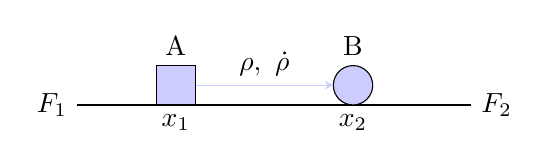
\begin{tikzpicture}
      \draw[thick] (0,0)node[left] {$F_1$} -- (5,0)node[right] {$F_2$};
      \filldraw[fill=blue!20] (1,0) -- (1,.5) -- (1.5,.5) -- (1.5,0) -- cycle;
      \node at (1.25,.5) [above] {A};
      \node at (1.25,0) [below] {$x_1$};
      \filldraw[fill=blue!20] (3.5,.25) circle (.25);
      \node at (3.5,.5) [above] {B};
      \node at (3.5,0) [below] {$x_2$};
      \draw[blue!20,->,>=stealth] (1.5,.25) -- (3.25,.25)node[pos=.5,above,black] {$\rho,\ \dot{\rho}$};
    \end{tikzpicture}
    \caption{运动系统}
    \label{fig:exercise-LDS}
  \end{figure}
\end{problemset}
\chapter{\textup{Kalman}滤波基础}\label{ch:kalman-filter}
\begin{introduction}
  \item 线性离散系统的\textup{Kalman}滤波
  \item 最优预测
  \item 最优平滑
\end{introduction}
\section{线性离散系统的\textup{Kalman}滤波}
Kalman滤波所做的包括\CJKunderdot{时间预测}和\CJKunderdot{测量更新}两方面,例如下面这道题
\begin{example}\label{ex:temperature-predict}
  某地区夏季夜间温度基本稳定.现已知0:00的温度为$20.0\pm 0.1^\circ\textup{C}$,预测
  下一点钟的温度也为$20.0^\circ\textup{C}$.在1:00时,用温度计量测的温度为$20.7\pm 0.2^\circ\textup{C}$.
\end{example}
我们可以建立该离散动态系统的模型如下:
\[
  \bm{X}(k)=\bm{\varPhi}_{k,k-1}\bm{X}(k-1)+\bm{w}(k-1),\quad \bm{Z}(k)=\bm{H}_k\bm{X}(k)+\bm{\varDelta}(k)
\]
随机模型
\[
  E[\bm{w}(k)]=\bm{0},\quad\Cov[\bm{w}(k),\bm{w}(j)]=\bm{D}_w(k)\delta_{kj}
\]
\[
  E[\bm{\varDelta}(k)]=\bm{0},\quad\Cov[\bm{\varDelta}(k),\bm{\varDelta}(j)]=\bm{D}_\varDelta(k)\delta_{kj}
\]
\[
  \Cov[\bm{w}(k),\bm{\varDelta}(j)]=\bm{0}
\]
此外,已知$\hat{\bm{X}}(0)$,且有
\begin{equation}\label{eq:initial-no-unbiasedness}
  \textcolor{magenta}{E[\hat{\bm{X}}(0)]=E[\bm{X}(0)],\quad\text{是无偏估计}}
\end{equation}
\begin{note}
  请留意上面这个式子,接下来的推导中会用到!
\end{note}
我们要做的就是
\[
  \begin{cases}
    \text{时间预测:用}\bm{Z}(1),\ \bm{Z}(2),\ldots,\ \bm{Z}(k-1)\text{来估计}\bm{X}(k)\longrightarrow\textcolor{magenta}{\hat{\bm{X}}(k,k-1)}\\
    \text{测量更新:用}\bm{Z}(1),\ \bm{Z}(2),\ldots,\ \bm{Z}(k-1),\ \bm{Z}(k)\text{来估计}\bm{X}(k)\longrightarrow\textcolor{magenta}{\hat{\bm{X}}(k)}
  \end{cases}
\]
\subsection{时间预测}
对于时间预测估计,有
\begin{equation}
  \hat{\bm{X}}(k,k-1)=E[\bm{X}(k)\mid\bm{Z}(1)\bm{Z}(2)\ldots\bm{Z}(k-1)]
\end{equation}
将差分方程$\bm{X}(k)=\bm{\varPhi}_{k,k-1}\bm{X}(k-1)+\bm{w}(k-1)$代入,再根据期望的线性性,不难推导得出
\begin{align*}
  \hat{\bm{X}}(k,k-1)&=\bm{\varPhi}_{k,k-1}E[\bm{X}(k-1)\mid\bm{Z}(1)\bm{Z}(2)\ldots\bm{Z}(k-1)]+\cancelto{0}{E[\bm{w}(k-1)\mid\bm{Z}(1)\bm{Z}(2)\ldots\bm{Z}(k-1)]}\\
  &=\bm{\varPhi}_{k,k-1}E[\bm{X}(k-1)\mid\bm{Z}(1)\bm{Z}(2)\ldots\bm{Z}(k-1)]\\
  &=\bm{\varPhi}_{k,k-1}\hat{\bm{X}}(k-1)
\end{align*}
由此我们得到
\begin{equation}\label{eq:one-step-predict}
  \hat{\bm{X}}(k,k-1)=\bm{\varPhi}_{k,k-1}\hat{\bm{X}}(k-1)
\end{equation}
在例题\ref{ex:temperature-predict}中有$\bm{X}(0)$已知,我们便可以由上式推知$\hat{\bm{X}}(1,0)$,这种方法叫作\uline{一步预测}.

一步预测估计的无偏性和有效性如何?即它的随机模型如何?现定义一步预测的\colorbox{yellow!20}{估计误差}为
\begin{equation}
  \Delta\hat{\bm{X}}(k,k-1)=\bm{X}(k)-\hat{\bm{X}}(k,k-1)
\end{equation}
将\eqref{eq:one-step-predict}和离散模型差分方程
\[
  \bm{X}(k)=\bm{\varPhi}_{k,k-1}\bm{X}(k-1)+\bm{w}(k-1)
\]代入可得
\begin{align*}
  \Delta\hat{\bm{X}}(k,k-1)&=\bm{\varPhi}_{k,k-1}\bm{X}(k-1)+\bm{w}(k-1)-\bm{\varPhi}_{k,k-1}\hat{\bm{X}}(k-1)\\
  &=\bm{\varPhi}_{k,k-1}\Delta\bm{\hat{X}}(k-1)+\bm{w}(k-1)
\end{align*}
求期望,不难看出:
\begin{equation}\label{eq:unbiased-or-not}
  E[\Delta\hat{\bm{X}}(k,k-1)]=\bm{\varPhi}_{k,k-1}E[\Delta\bm{\hat{X}}(k-1)]
\end{equation}
\textcolor{magenta}{\HandRight}一步预测的无偏性完全由接下来我们推导的测量更新的无偏性决定!(详见后文,一步预测估计是无偏的)

现在来推导方差函数:
\begin{align*}
  D[\Delta\hat{\bm{X}}(k,k-1)]&:=\bm{D}_{\hat{X}}(k,k-1)=E\left[\Delta\hat{\bm{X}}(k,k-1)\Delta\hat{\bm{X}}^\mT(k,k-1)\right]\\
  &=\bm{\varPhi}_{k,k-1}E\left[\Delta\bm{\hat{X}}(k-1)\Delta\bm{\hat{X}}^\mT(k-1)\right]\bm{\varPhi}^\mT_{k,k-1}+E\left[\bm{w}(k-1)\bm{w}^\mT(k-1)\right]\\
  &\ {}+E\left[\bm{w}(k-1)\Delta\bm{\hat{X}}^\mT(k-1)\right]\bm{\varPhi}^\mT_{k,k-1}+\bm{\varPhi}_{k,k-1}E\left[\Delta\bm{\hat{X}}(k-1)\bm{w}^\mT(k-1)\right]
\end{align*}
式中最后两项显然等于0,因为已经推导过\uwave{系统噪声和观测噪声无关}.最终我们可以得到
\begin{equation}\label{eq:kalman-time-predict-variance}
  \bm{D}_{\hat{X}}(k,k-1)=\bm{\varPhi}_{k,k-1}\bm{D}_{\hat{X}}(k-1)\bm{\varPhi}^\mT_{k,k-1}+\bm{D}_{w}(k-1)
\end{equation}
我们做一个小小的阶段性总结吧:
\begin{conclusion}
  有关时间预测估计的相关结论:
  \begin{enumerate}
    \item 数学模型:$\displaystyle \hat{\bm{X}}(k,k-1)=\bm{\varPhi}_{k,k-1}\hat{\bm{X}}(k-1)$;
    \item 随机模型:
    \begin{enumerate}
      \item 期望:$\displaystyle E[\Delta\bm{\hat{X}}(k,k-1)]=\bm{0}$;
      \item 方差:$\displaystyle \bm{D}_{\hat{X}}(k,k-1)=\bm{\varPhi}_{k,k-1}\bm{D}_{\hat{X}}(k-1)\bm{\varPhi}^\mT_{k,k-1}+\bm{D}_w(k-1)$.
    \end{enumerate}
  \end{enumerate}
\end{conclusion}
\subsection{测量更新}
下面我们基于最小方差估计(详见小节\ref{sec:MMSE-estimation})来进行估计:我们曾知道MMSE估计结果是验后方差,我们的先验信息
就来自方才推导的时间预测估计结果$\hat{\bm{X}}(k,k-1)$即成立
\[
  E[\bm{X}(k)]=\hat{\bm{X}}(k,k-1).
\]
进一步地,基于线性模型的MMSE估计,我们有
\[
  \hat{\bm{X}}=E(\bm{X})+\bm{D}_{XZ}\bm{D}_Z^{-1}(\bm{Z}-E(\bm{Z}))
\]
将所有已知值代入,整理得
\begin{equation}\label{eq:measurement-update-equation}
  \boxed{\hat{\bm{X}}(k)=\hat{\bm{X}}(k,k-1)+\underbrace{\bm{D}_{\hat{X}}(k,k-1)\bm{H}_k^\mT\left(\bm{H}_k\bm{D}_{\hat{X}}(k,k-1)\bm{H}_k^\mT+\bm{D}_{\varDelta}(k)\right)^{-1}}_{\bm{K}_k}\underbrace{\left[\bm{Z}(k)-\bm{H}_k\hat{\bm{X}}(k,k-1)\right]}_{\bm{V}(k,k-1)}
}\end{equation}
称上式中$\bm{K}_k$为\CJKunderdot{增益矩阵},上式中$\bm{V}(k,k-1)$为\CJKunderdot{预测残差}或\CJKunderdot{新息}.
那么庞大的测量更新估计结果可以被表示为
\begin{equation}
  \hat{\bm{X}}(k)=\hat{\bm{X}}(k,k-1)+\bm{K}_k\bm{V}(k,k-1)
\end{equation}
现在来推导随机模型:对上式求期望,有
\[
  E[\hat{\bm{X}}(k)]=\underset{\textcolor{magenta}{\text{\ding{172}}}}{E[\hat{\bm{X}}(k,k-1)]}+\underset{\textcolor{magenta}{\text{\ding{173}}}}{\bm{K}_kE[\bm{V}(k,k-1)}]
\]
\begin{enumerate}
  \item[\textcolor{magenta}{\ding{172}}] 时间预测的期望,依赖于$E[\hat{\bm{X}}(k,k-1)]\xlongequal{?}E[\bm{X}(k)]$;
  \item[\textcolor{magenta}{\ding{173}}] 预测残差的期望,依赖于$E[\bm{Z}(k)]-E[\bm{H}_k\hat{\bm{X}}(k,k-1)]=\bm{H}_k(E[\bm{X}(k)]-E[\bm{\hat{X}}(k,k-1)])$.
\end{enumerate}
也就是说,决定“测量更新估计为无偏估计”的两个要素都取决于
\[
  E[\Delta\hat{\bm{X}}(k,k-1)]=E[\hat{\bm{X}}(k,k-1)]-E[\bm{X}(k)]\xlongequal{\text{等式}\eqref{eq:unbiased-or-not}}E[\hat{\bm{X}}(k-1)]-E[\bm{X}(k-1)]\xlongequal{?}\bm{0}
\]
这也是之前提到的“时间预测估计为无偏估计”的决定因素,它们之间形成了一条“链”:
\begin{figure}[H]
  \centering
  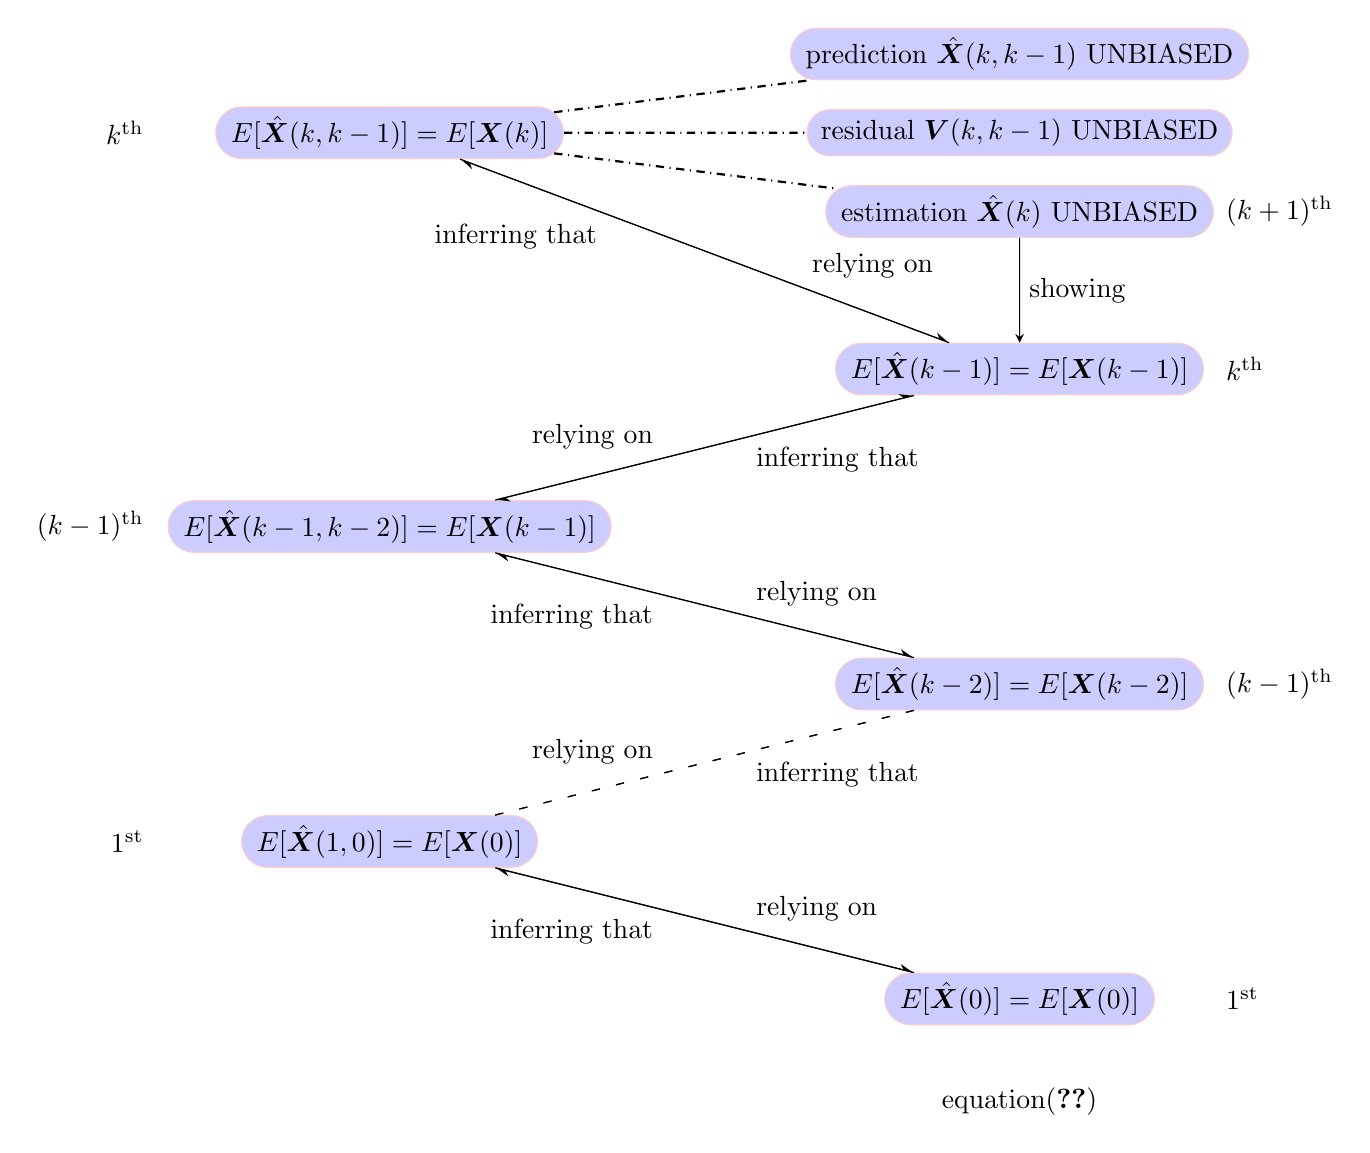
\begin{tikzpicture}
    \node[Txt] (text1) at (0,0) {$E[\hat{\bm{X}}(k,k-1)]=E[\bm{X}(k)]$};
    \node[Txt] (text2) at (8,1) {prediction\ $\hat{\bm{X}}(k,k-1)$\ UNBIASED};
    \node[Txt] (text3) at (8,0) {residual\ $\bm{V}(k,k-1)$\ UNBIASED};
    \node[Txt] (text4) at (8,-1) {estimation\ $\hat{\bm{X}}(k)$\ UNBIASED};
    \begin{scope}[dash dot,thick]
      \draw (text1) -- (text2);
      \draw (text1) -- (text3);
      \draw (text1) -- (text4);
    \end{scope}
    \node[Txt] (pro1) at (8,-3) {$E[\hat{\bm{X}}(k-1)]=E[\bm{X}(k-1)]$};
    \draw[->,>=stealth] (text4) -- (pro1) node[pos=.5,right] {showing};
    \node[Txt] (pro2) at (0,-5) {$E[\hat{\bm{X}}(k-1,k-2)]=E[\bm{X}(k-1)]$};
    \node[Txt] (pro3) at (8,-7) {$E[\hat{\bm{X}}(k-2)]=E[\bm{X}(k-2)]$};
    \node[Txt] (pro4) at (0,-9) {$E[\hat{\bm{X}}(1,0)]=E[\bm{X}(0)]$};
    \node[Txt] (pro5) at (8,-11) {$E[\hat{\bm{X}}(0)]=E[\bm{X}(0)]$};
    \begin{scope}[->,arrows = {-Stealth[harpoon]}]
      \draw (text1) -- (pro1) node[pos=.7,above right] {relying on};
      \draw (pro1) -- (text1) node[pos=.7,below left] {inferring that};
      \draw (pro1) -- (pro2) node[pos=.6,above left] {relying on};
      \draw (pro2) -- (pro1) node[pos=.6,below right] {inferring that};
      \draw (pro2) -- (pro3) node[pos=.6,above right] {relying on};
      \draw (pro3) -- (pro2) node[pos=.6,below left] {inferring that};
      \draw (pro4) -- (pro5) node[pos=.6,above right] {relying on};
      \draw (pro5) -- (pro4) node[pos=.6,below left] {inferring that};
    \end{scope} 
    \draw[loosely dashed] (pro3) -- (pro4) node[pos=.6,above left] {relying on};
    \draw[loosely dashed] (pro4) -- (pro3) node[pos=.6,below right] {inferring that};
    \node at (pro5) [below=1cm] {equation\eqref{eq:unbiased-or-not}};
    \node at (pro5) [right=2.5cm] {$1^{\text{st}}$};
    \node at (pro3) [right=2.5cm] {$(k-1)^{\text{th}}$};
    \node at (pro1) [right=2.5cm] {$k^{\text{th}}$};
    \node at (text4) [right=2.5cm] {$(k+1)^{\text{th}}$};
    \node at (pro4) [left=3cm] {$1^{\text{st}}$};
    \node at (pro2) [left=3cm] {$(k-1)^{\text{th}}$};
    \node at (text1) [left=3cm] {$k^{\text{th}}$};
  \end{tikzpicture}
\end{figure}
这条链最终指向了我们规定的式\eqref{eq:unbiased-or-not},也就是说,如果一开始$\hat{\bm{X}}(0)$是$t_0$时刻状态
的无偏估计,那么下面的命题通通成立:
\begin{itemize}
  \item 时间预测估计是无偏估计;
  \item 测量更新估计是无偏估计;
  \item 预测残差是无偏估计.
\end{itemize}

回到正题,我们同样可以定义误差来源
\begin{equation}
  \Delta\hat{\bm{X}}(k):=\bm{X}(k)-\hat{\bm{X}(k)}=(\bm{I}-\bm{K}_k\bm{H}_k)\Delta\hat{\bm{X}}(k,k-1)-\bm{K}_k\bm{\varDelta}(k)
\end{equation}
推得方差函数(此处省略推导过程)
\begin{equation}
  \bm{D}_{\hat{X}}(k)=(\bm{I}-\bm{K}_k\bm{H}_k)\bm{D}_{\hat{X}}(k,k-1)(\bm{I}-\bm{K}_k\bm{H}_k)^\mT+\bm{K}_k\bm{D}_{\varDelta}(k)\bm{K}_k^\mT
\end{equation}
上式保持了方差阵的正定性,此外,我们还可以根据矩阵的恒等关系\footnote{做个记号,有时间就推一下}整理出
\begin{equation}
  \bm{D}_{\hat{X}}(k)=(\bm{I}-\bm{K}_k\bm{H}_k)\bm{D}_{\hat{X}}(k,k-1)
\end{equation}
上式则更方便计算,但失去了方差阵的正定性.或者我们求逆,得到
\begin{equation}
  \bm{D}_{\hat{X}}^{-1}(k)=\bm{D}_{\hat{X}}^{-1}(k,k-1)+\bm{H}_k\bm{D}_{\varDelta}^{-1}(k)\bm{H}_k^\mT
\end{equation}
上式可以理解为:\uline{测量更新的权由先验信息的权和观测值的权共同决定}.

同样做总结如下:
\begin{conclusion}
  有关测量更新估计的相关结论:
  \begin{enumerate}
    \item 数学模型:$\displaystyle \hat{\bm{X}}(k)=\hat{\bm{X}}(k,k-1)+\bm{K}_k\bm{V}(k,k-1)$;
    \item 随机模型:
    \begin{enumerate}
      \item 期望:$\displaystyle E[\Delta\bm{\hat{X}}(k)]=\bm{0}$;
      \item 方差的三种形式:
      \begin{enumerate}
      \item $\displaystyle \bm{D}_{\hat{X}}(k)=(\bm{I}-\bm{K}_k\bm{H}_k)\bm{D}_{\hat{X}}(k,k-1)(\bm{I}-\bm{K}_k\bm{H}_k)^\mT+\bm{K}_k\bm{D}_{\varDelta}(k)\bm{K}_k^\mT$;
      \item $\displaystyle \bm{D}_{\hat{X}}(k)=(\bm{I}-\bm{K}_k\bm{H}_k)\bm{D}_{\hat{X}}(k,k-1)$;
      \item $\displaystyle \bm{D}_{\hat{X}}^{-1}(k)=\bm{D}_{\hat{X}}^{-1}(k,k-1)+\bm{H}_k\bm{D}_{\varDelta}^{-1}(k)\bm{H}_k^\mT$.
      \end{enumerate}
    \end{enumerate}
  \end{enumerate}
\end{conclusion}
回到例题\ref{ex:temperature-predict},我们已知$X(0)=20.0$,\ $\sigma_X(0)=0.1$,\ $X(k)=X(k-1)+w(k-1)$,故$\varPhi_{k,k-1}=1$,而
\[
    \hat{X}(1,0)=\hat{X}(0),\quad D_{\hat{X}}(1,0)=D_{\hat{X}}(0)+D_w(0)
\]
由于$Z(k)=X(k)+\varDelta(k)$,故$H_1=1$,将$K_1$代入,解得
\[
    \hat{X}(1)=\hat{X}(1,0)+K_1[Z(1)-H_1\hat{X}(1,0)]=20.5.
\]
\subsection{存在控制输入的情况}
由于控制输入项$\bm{u}(t)$并不是随机量且不影响观测模型,所以只有时间预测的结果会发生改变:
\begin{equation}
  \hat{\bm{X}}(k,k-1)=\bm{\varPhi}_{k,k-1}\hat{\bm{X}}(k-1)+\bm{\Omega}(k-1)
\end{equation}
\subsection{Kalman滤波与递推最小二乘估计}
回到小节\ref{sec:recursion-LS},品味定理\ref{thm:recursion-LS}中有关增益矩阵和预测残差的定义,就能发现
Kalman滤波和递推最小二乘估计的很强的相似性,下面就来推导他们之间的关系:考虑系统模型
\[
  \dot{\bm{X}}(t)=\bm{A}(t)\bm{X}(t)+\bm{C}(t)\bm{e}(t)
\]
当$\bm{A}=\bm{0}$,\ $\bm{e}(t)=0$时,模型退化成
\[
  \begin{cases}
    \dot{\bm{X}}(t)=\bm{0}\\
    \bm{X}(k)=\bm{X}(k-1)
  \end{cases}
\]
这使得此时的一步预测模型:
\[
  \hat{\bm{X}}(k,k-1)=\hat{\bm{X}}(k-1),
\]
\[
  \bm{D}_{\hat{X}}(k,k-1)=\bm{D}_{\hat{X}}(k-1),
\]
测量更新模型
\begin{equation}
  \hat{\bm{X}}(k)=\hat{\bm{X}}(k-1)+\bm{K}_k\left[\bm{Z}(k)-\bm{H}_k\hat{\bm{X}}(k-1)\right],
\end{equation}
\begin{equation}
  \bm{K}_k=\bm{D}_{\hat{X}}(k-1)\bm{H}_k^\mT\left(\bm{H}_k\bm{D}_{\hat{X}}(k-1)\bm{H}_k^\mT+\bm{D}_{\varDelta}(k)\right)^{-1}
\end{equation}
这就是递推最小二乘.
\begin{proposition}[Kalman滤波与递推最小二乘估计的关系]
  当系统状态为随机常数时,Kalman滤波退化为递推最小二乘估计.
\end{proposition}
\subsection{Kalman滤波与单历元最小二乘估计}
如果我们将预测值作为与观测方程同一历元的一个\textcolor{magenta}{虚拟观测值},联立
\begin{equation}
  \begin{cases}
    \hat{\bm{X}}(k,k-1)=\hat{\bm{X}}(k)+\bm{\varDelta}_{\hat{X}}(k,k-1)\\
    \bm{Z}(k)=\bm{H}_k\hat{\bm{X}}(k)+\bm{\varDelta}(k)
  \end{cases}
\end{equation}
随机模型
\begin{equation}
  \bm{D}=\begin{bmatrix}
    \bm{D}_{\hat{X}}(k,k-1)& \\
     &\bm{D}_\varDelta
  \end{bmatrix}
\end{equation}
那么权阵
\[
  \bm{W}=\begin{bmatrix}
    \bm{D}_{\hat{X}}^{-1}& \\
     &\bm{D}_{\varDelta}^{-1}
  \end{bmatrix}
\]
根据法方程,
\begin{align*}
  \begin{bmatrix}
    \bm{I}&\bm{H}^\mT
  \end{bmatrix}
  \begin{bmatrix}
    \bm{D}_X^{-1}& \\
     &\bm{D}_\varDelta^{-1}
  \end{bmatrix}
  \begin{bmatrix}
    \bm{I}\\
    \bm{H}
  \end{bmatrix}\bm{X}&=
  \begin{bmatrix}
    \bm{I}&\bm{H}
  \end{bmatrix}
  \begin{bmatrix}
    \bm{D}_X^{-1}& \\
     &\bm{D}_\varDelta^{-1}
  \end{bmatrix}
  \begin{bmatrix}
    \hat{\bm{X}}(k,k-1)\\
    \bm{Z}(k)
  \end{bmatrix}\\
  \left(\bm{D}_X^{-1}+\bm{H}^\mT\bm{D}_\varDelta^{-1}\bm{H}\right)\bm{X}&=\left[\bm{D}_X^{-1}\hat{\bm{X}}(k,k-1)+\bm{H}^\mT\bm{D}_\varDelta^{-1}\bm{Z}(k)\right]\\
  \left(\bm{W}_x+\bm{H}^\mT\bm{W}_\varDelta\bm{H}\right)\bm{X}&=\left[\bm{W}_x\hat{\bm{X}}(k,k-1)+\bm{H}^\mT\bm{W}_\varDelta\bm{Z}(k)\right]
\end{align*}
相比于最小二乘估计,我们多了一组观测值的信息.\\
\textcolor{magenta}{\HandRight}那么这组观测值的精度信息$\bm{D}_{\hat{X}}$如何?\\
当这组观测值的精度非常差时,\ $\bm{D}_{\hat{X}}(k,k-1)=\infty$,此时就是单历元最小二乘估计;当
这组观测值可靠性很强时,\ $\bm{D}_{\hat{X}}(k,k-1)=\bm{0}$,则构成了\CJKunderdot{强约束条件},模型也就成了\colorbox{yellow!20}{附有限制条件的间接平差模型}.
\section{线性Kalman滤波做最优预测和平滑}\label{sec:Kalman-predict-smooth}
当无观测值$\bm{Z}(k)$时,\ $\bm{D}_\varDelta(k)\to\infty$,\ $\bm{K}_k\to 0$,此时
\[
  \hat{\bm{X}}(k)=\hat{\bm{X}}(k,k-1),
\]
且有一步预测
\begin{align*}
  \hat{\bm{X}}(k+1,k)&=\hat{\bm{X}}(k+1)=\bm{\varPhi}_{k+1,k}\hat{\bm{X}}(k)\\
  &=\bm{\varPhi}_{k+1,k}\hat{\bm{X}}(k,k-1)
\end{align*}
那么递推得到$k$时刻到$\l$时刻的预测模型,即\textcolor{magenta}{最优预测}:
\begin{equation}
  \hat{\bm{X}}(\l,k)=\bm{\varPhi}_{\l,k}\hat{\bm{X}}(k)
\end{equation}
\begin{equation}
  \bm{D}_{\hat{X}}(\l,k)=\bm{\varPhi}_{\l,k}\bm{D}_{\hat{X}}(k)\bm{\varPhi}_{\l,k}^\mT+\sum_{i=k+1}^\l\bm{\varPhi}_{\l,i}\bm{D}_w(i-1)\bm{\varPhi}_{\l,i}^\mT
\end{equation}
这意味着如果没有观测更新,那么误差就会不断积累.

平滑(smoothing)是发生在预测之后的事,它是用\CJKunderdot{所有}观测值再来重新估计每一个状态量,即
\[
  E\left(\bm{X}(j)\mid\bm{Z}(1)\bm{Z}(2)\ldots\bm{Z}(j)\ldots\bm{Z}(\l)\right)
\]
这样处理得到的结果的方差会比预测得到的方差小很多、光滑很多,也是因为如此这种预测叫做光滑.

平滑分三种
\begin{enumerate}
  \item 固定区间平滑(Fixed-Interval Smoothing)
  \item 固定滞后平滑(Fixed-Lag Smoothing)
  \item 固定点平滑(Fixed-Point Smoothing)
\end{enumerate}
上一段落介绍的是最一般的固定区间平滑,我个人比较喜欢下面的组图来解释三种平滑的区别
\begin{figure}[H]
  \centering
  \subfigure[固定区间平滑]{\label{subfig:intesmooth}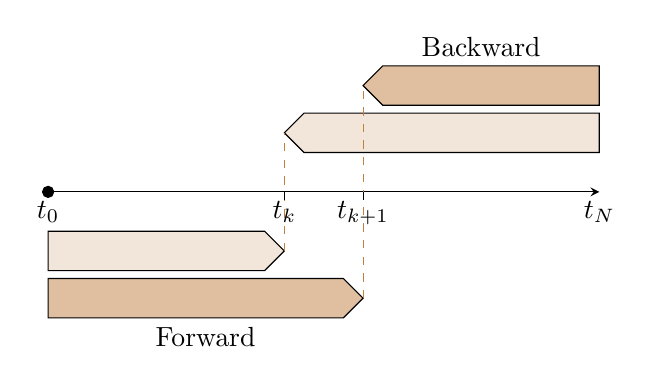
\begin{tikzpicture}
    \draw[fill=black] (0,0) circle (2pt);
    \draw[->,>=stealth] (0,0) node[below] {$t_0$} -- (7,0) node[below] {$t_N$};
    \node at (3,0) [below] {$t_k$};
    \node at (4,0) [below] {$t_{k+1}$};
    \draw[fill=brown!20,draw=black] (0,-.5) -- (2.75,-.5) -- (3,-.75) -- (2.75,-1) -- (0,-1) -- cycle;
    \draw[fill=brown!50,draw=black] (0,-1.1) -- (3.75,-1.1) -- (4,-1.35) -- (3.75,-1.6) -- (0,-1.6) -- cycle;
    \draw[fill=brown!20,draw=black] (7,.5) -- (3.25,.5) -- (3,.75) -- (3.25,1) -- (7,1) -- cycle;
    \draw[fill=brown!50,draw=black] (7,1.1) -- (4.25,1.1) -- (4,1.35) -- (4.25,1.6) -- (7,1.6) -- cycle;
    \node at (2,-1.6) [below] {Forward};
    \node at (5.5,1.6) [above] {Backward};
    \begin{scope}[dashed,brown]
      \draw (3,-.75) -- (3,.75);
      \draw (4,-1.35) -- (4,1.35);
    \end{scope}
    \foreach \i in {3,4}
    {
      \draw (\i,0) -- (\i,-.1);
    }
  \end{tikzpicture}}\\
  \subfigure[固定点平滑]{\label{subfig:pointsmooth}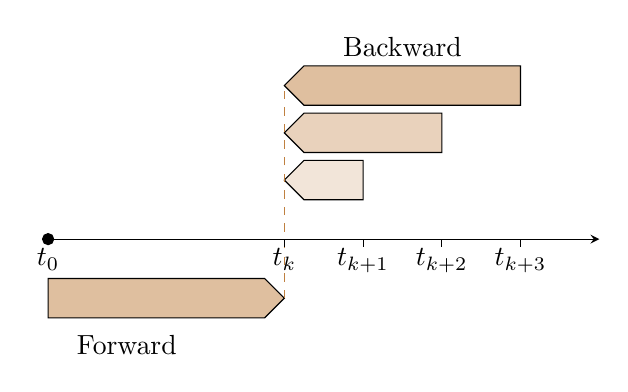
\begin{tikzpicture}
    \draw[fill=black] (0,0) circle (2pt);
    \draw[->,>=stealth] (0,0) node[below] {$t_0$} -- (7,0);
    \node at (3,0) [below] {$t_k$};
    \node at (4,0) [below] {$t_{k+1}$};
    \node at (5,0) [below] {$t_{k+2}$};
    \node at (6,0) [below] {$t_{k+3}$};
    \draw[fill=brown!50,draw=black] (0,-.5) -- (2.75,-.5) -- (3,-.75) -- (2.75,-1) -- (0,-1) -- cycle;
    \draw[fill=brown!20,draw=black] (4,.5) -- (3.25,.5) -- (3,.75) -- (3.25,1) -- (4,1) -- cycle;
    \draw[fill=brown!35,draw=black] (5,1.1) -- (3.25,1.1) -- (3,1.35) -- (3.25,1.6) -- (5,1.6) -- cycle;
    \draw[fill=brown!50,draw=black] (6,1.7) -- (3.25,1.7) -- (3,1.95) -- (3.25,2.2) -- (6,2.2) -- cycle;
    \node at (1,-1.1) [below] {Forward};
    \node at (4.5,2.2) [above] {Backward};
    \begin{scope}[dashed,brown]
      \draw (3,-.75) -- (3,1.95);
    \end{scope}
    \foreach \i in {3,4,5,6}
    {
      \draw (\i,0) -- (\i,-.1);
    }
  \end{tikzpicture}}\\
  \subfigure[固定滞后平滑]{\label{subfig:lagsmooth}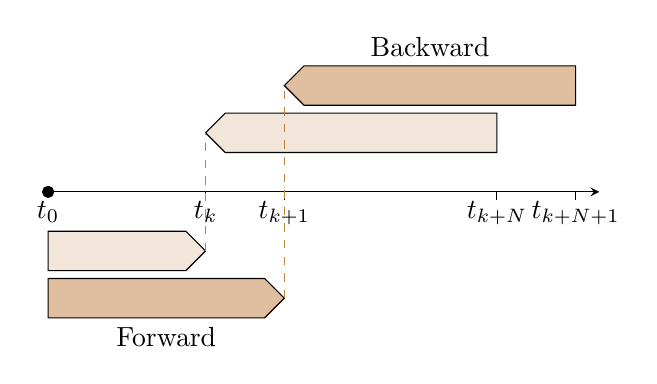
\begin{tikzpicture}
    \draw[fill=black] (0,0) circle (2pt);
    \draw[->,>=stealth] (0,0) node[below] {$t_0$} -- (7,0);
    \foreach \i in {2,3,5.7,6.7}
    {
      \draw (\i,0) -- (\i,-.1);
    }
    \node at (2,0) [below] {$t_k$};
    \node at (3,0) [below] {$t_{k+1}$};
    \node at (5.7,0) [below] {$t_{k+N}$};
    \node at (6.7,0) [below] {$t_{k+N+1}$};
    \draw[fill=brown!20,draw=black] (0,-.5) -- (1.75,-.5) -- (2,-.75) -- (1.75,-1) -- (0,-1) -- cycle;
    \draw[fill=brown!50,draw=black] (0,-1.1) -- (2.75,-1.1) -- (3,-1.35) -- (2.75,-1.6) -- (0,-1.6) -- cycle;
    \draw[fill=brown!20,draw=black] (5.7,.5) -- (2.25,.5) -- (2,.75) -- (2.25,1) -- (5.7,1) -- cycle;
    \draw[fill=brown!50,draw=black] (6.7,1.1) -- (3.25,1.1) -- (3,1.35) -- (3.25,1.6) -- (6.7,1.6) -- cycle;
    \node at (1.5,-1.6) [below] {Forward};
    \node at (4.85,1.6) [above] {Backward};
    \begin{scope}[dashed,brown]
      \draw (2,-.75) -- (2,.75);
      \draw (3,-1.35) -- (3,1.35);
    \end{scope}
  \end{tikzpicture}}
  \caption{三种平滑手段}
  \label{fig:smoothing}
\end{figure}
图\ref{fig:smoothing}\subref{subfig:intesmooth}描述了基于前-后滤波器,利用从$t_0$到$t_N$的所有观测值来估计任意时刻$t_i$的
状态的估计方法,图中展示了$t_k$和$t_{k+1}$两个时刻的状态估计.

图\ref{fig:smoothing}\subref{subfig:pointsmooth}用不断增加的平滑窗,即不断增加的观测值来估计某一兴趣时刻$t_k$的状态.

图\ref{fig:smoothing}\subref{subfig:lagsmooth}用从$t_0$到$t_{i+N}$的观测值来估计任意时刻$t_i$的状态,其中$N$是给定的\uwave{延后时长},图中
展示了$t_k$和$t_{k+1}$时刻的状态估计.
\begin{problemset}
  \item 在已知坐标(平面)的两个基站设置仪器对运动目标P进行持续观测,观测值为基站到
  目标P的距离,观测方程为
  \[
    \rho_i=\sqrt{(X_{S_i}-X)^2+(Y_{S_i}-Y)^2}+\delta t+s+\varDelta^i,\quad i=1,2
  \]
  其中$\rho_i$为距离观测值,\ $(X_{S_i},Y_{S_i})^\mT$为基站的坐标,\ $(X,Y)^\mT$为目标点的坐标,\ $\delta t$为接收机钟差,\ $s$为
  观测值中的系统误差,\ $\varDelta$为随机误差.

  为了用Kalman滤波估计接收机的位置,自设所需变量解决以下问题:
  \begin{enumerate}
    \item 用\textup{PV}(Position and Velocity)模型来描述接收机$(X,Y)$的变化规律,给出微分方程和离散的状态方程(包括随机模型);
    \item 若将$\delta t$变化规律描述为随机游走,给出微分方程和离散的状态方程(包括随机模型);
    \item 将$s$的描述为随机常数,给出微分方程和离散的状态方程(包括随机模型);
    \item 将观测方程线性化,与以上状态对应,将观测方程表示为向量和矩阵的形式.
  \end{enumerate}
  \item 系统的运动规律可表示为$\dot{X}(t)=X^2(t)+e(t)$,其中$e(t)$为零均值白噪声,均方值$\sigma_e^2=0.1$.观测方程
  $Z(k)=\cos[X(k)]+\varDelta(k)$,其中$\varDelta(k)$为零均值白噪声,\ $\varDelta(k)$与$e(t)$不相关.自设变量,用扩展的
  Kalman滤波解决以下问题.
  \begin{enumerate}
    \item 给出状态转移矩阵和离散化后的状态方程以及系统噪声方差;
    \item 已知$X(0)$,\ $\sigma_X^2(0)$,给出$\hat{X}(1,0)$和其方差的表达式;
    \item 已知$Z(1)$,\ $\sigma_{\varDelta}^2$,求新息$V(1,0)$,增益矩阵$K_1$和$\hat{X}(1)$的表达式.
  \end{enumerate}
\end{problemset}
\chapter{改进的\textup{Kalman}滤波}
\begin{introduction}
  \item 观测值逐次更新法
  \item 扩展的Kalman滤波
  \item 信息滤波
  \item 平方根分解
\end{introduction}
章节标题中“改进”意为\emph{改进了算法}的,相比于最一般的Kalman滤波,改进的算法针对计算机计算
做了很大程度上的优化.
\section{观测值逐次更新的Kalman滤波}\label{sec:kf-measurement-update}
将$\l$个观测值中的第$j$个量拎出来($j=1,2,\ldots,\l$)
\[
  \underset{1\times 1}{Z_j(k)}=\underset{1\times n}{\bm{h}_j}\underset{n\times 1}{\bm{X}(k)}+\underset{1\times 1}{\varDelta_j(k)}\qquad \underset{1\times 1}{d_j(k)}
\]
每一个观测值都可以对时间预测$\hat{\bm{X}}(k,k-1)$进行更新,因此,我们考虑从$Z_1(k)$\CJKunderdot{逐次更新}时间预测值,一直到$Z_\l(k)$,具体步骤:
\begin{itemize}
  \item 拿$Z_1(k)$更新$\hat{\bm{X}}(k,k-1)$至$\hat{\bm{X}}^{[1]}(k)$(随机模型更新至$\bm{D}^{[1]}_{\hat{X}}(k)$);
  \item 拿$Z_2(k)$更新$\hat{\bm{X}}^{[1]}(k)$至$\hat{\bm{X}}^{[2]}(k)$(随机模型更新至$\bm{D}^{[2]}_{\hat{X}}(k)$);
  \item $\cdots$
  \item 拿$Z_\l(k)$更新至$\hat{\bm{X}}^{[\l]}(k)$(随机模型更新至$\bm{D}^{[\l]}_{\hat{X}}(k)$).
\end{itemize}
\begin{theorem}[观测值逐次更新一般公式]\label{thm:update-several-times}
  第$j$次更新时,有
  \begin{equation}
    V_j(k,k-1)=Z_j(k)-\bm{h}_j\hat{\bm{X}}^{[j-1]}(k)
  \end{equation}
  \begin{equation}\label{eq:gain-improve}
    \bm{K}_k^{[j]}(k)=\bm{D}_{\hat{X}}^{[j-1]}(k)\bm{h}_j^\mT\bigg/\left(\bm{h}_j\bm{D}_{\hat{X}}^{[j-1]}(k)\bm{h}_j^\mT+d_j(k)\right)
  \end{equation}
  \begin{equation}
    \hat{\bm{X}}^{[j]}(k)=\hat{\bm{X}}^{[j-1]}(k)+\bm{K}_k^{[j]}V_j(k,k-1)
  \end{equation}
  \begin{equation}
    \bm{D}_{\hat{X}}^{[j]}(k)=\left(\bm{I}-\bm{K}_k^{[j]}\bm{h}_j(k)\right)\bm{D}_{\hat{X}}^{[j-1]}(k)
  \end{equation}
\end{theorem}
改进的关键就在于式\eqref{eq:gain-improve}:$\bm{K}_k$原来的计算需要求解一个$\l\times\l$维矩阵的逆,此处只需要算一个一维纯量的倒数;然而改进
的缺陷也在于此,纯量中包含的方差信息没有与其他观测值之间的协方差信息.
\begin{theorem}[矩阵的Cholesky分解]\label{thm:matrix-cholesky}
  如果矩阵$\bm{A}$为对称矩阵,且$\varDelta_k=\det\bm{A}_k>0$($\bm{A}_k$是$\bm{A}$顺序主子阵),那么有
  \[
    \bm{A}=\bm{L}\bm{L}^\mT
  \]
  这样的分解唯一,称作Cholesky分解.此处
  \[
    \bm{L}=(\bm{U}^*)^\mT\bm{D}^{1/2}
  \]
  是一个下三角阵.
\end{theorem}
如果考虑对观测协方差阵进行Cholescky分解,
\begin{equation}\label{eq:cholesky-for-variance}
  \bm{D}_\varDelta(k)=\bm{L}\bm{L}^\mT  
\end{equation}
就只需要$\sum_{i=1}^\l i$个浮点数位来储存数据,这显然比$\l\times\l$个数据
要小得多.

我们对\eqref{eq:cholesky-for-variance}式进行处理:
\[
  \bm{L}^{-1}\bm{D}_\varDelta(k)\left(\bm{L}^\mT\right)^{-1}=\bm{I}
\]
脑中瞬间闪过灵感——此式是一个协方差传播率的形式,受到启发,我们在原观测方程两边同时左乘$\bm{L}^{-1}$:
\begin{equation}
  \underbrace{\bm{L}^{-1}\bm{Z}(k)}_{\bm{Y}(k)}=\underbrace{\bm{L}^{-1}\bm{H}_k}_{\bm{H}'(k)}\bm{X}(k)+\underbrace{\bm{L}^{-1}\bm{\varDelta}(k)}_{\bm{\varDelta}'(k)}
\end{equation}
此时的
\begin{equation}
  \bm{D}_{\varDelta'}(k)=\bm{L}^{-1}\bm{D}_\varDelta(k)\left(\bm{L}^{-1}\right)^\mT=\bm{I}
\end{equation}
据此我们就得到了新观测模型
\begin{equation}
  \bm{Y}(k)=\bm{H}_k\bm{X}(k)+\bm{\varDelta}'(k)\qquad\bm{D}_{\varDelta'}(k)=\bm{I}
\end{equation}
\section{扩展的Kalman滤波}
\subsection{EKF的E}
扩展(Extended)意味着从线性到非线性的扩展,对线性化
过程中Taylor展开中心进行了选取,以减小线性化带来的误差.扩展的Kalman滤波的英文简写为EKF.

考虑非线性动态系统模型
\begin{gather*}
  \dot{\bm{X}}(t)=\bm{g}[\bm{X}(t),\bm{u}(t),\bm{e}(t)]\\
  \bm{Z}(k)=\bm{F}[\bm{X}(k)]+\bm{\varDelta}(k)
\end{gather*}
对于状态方程,其线性化具体步骤应见命题\ref{pro:linearization-of-nonlinear-system},展开中心
应该选取上一历元的测量更新值$\hat{\bm{X}}(k-1)$(如果是第一次预测,则选取初值$\bm{X}(0)$).而其
离散化应见定理\ref{thm:continuous-linear-system-solution}及下面的式\eqref{eq:discrete-system-equation-easy}.
对于观测方程,它的线性化展开中心则选取刚才的预测值:
\begin{gather*}
  \bm{Z}(k)=\bm{H}_k\bm{X}(k)+\underbrace{\left\{\bm{F}[\bm{X}^*(k)]-\bm{H}(k)\bm{X}^*(k)\right\}}_{\text{非随机部分}}+\bm{\varDelta}(k)\\
  \textcolor{magenta}{\bm{X}^*(k)=\hat{\bm{X}}(k,k-1)}
\end{gather*}
这样会导致新息很好算:
\begin{align*}
  \bm{V}(k,k-1)&=\bm{Z}(k)=\left\{\bm{F}[\bm{X}^*(k)]-\bm{H}(k)\bm{X}^*(k)\right\}+\bm{\varDelta}(k)\\
  &=\bm{Z}(k)-\bm{F}[\hat{\bm{X}}(k-1)].
\end{align*}
\subsection{EKF+测量逐次更新法}
现在我们将观测方程的线性化和观测值逐次更新法联系起来:
\[
  \bm{Z}(k)=\begin{bmatrix}
    Z_1(k)\\
    Z_2(k)\\
    \vdots\\
    Z_\l(k)
  \end{bmatrix}=\begin{bmatrix}
    f_1(\bm{X}(k))\\
    f_2(\bm{X}(k))\\
    \vdots\\
    f_\l(\bm{X}(k))
  \end{bmatrix}+\begin{bmatrix}
    \varDelta_1(k)\\
    \varDelta_2(k)\\
    \vdots\\
    \varDelta_\l(k)
  \end{bmatrix}
\]
如果需要做观测值逐次更新的Kalman滤波,就需要对每一组观测方程进行线性化,每一组的展开中心都可以重新考虑:
\begin{figure}[H]
  \centering
  \begin{tikzpicture}
    \node[Txt] (O1) at (0,0) {$Z_1=f_1(\bm{X})+\varDelta_1$};
    \node[Txt] (Oa1) at (8,0) {$Z_1=h_1\bm{X}+\varDelta_1+f_1(\bm{X}^*)-h_1\bm{X}^*$};
    \node[Txt] (O2) at (0,-1) {$Z_2=f_2(\bm{X})+\varDelta_2$};
    \node[Txt] (Oa2) at (8,-1) {$Z_2=h_2\bm{X}+\varDelta_2+f_2(\bm{X}^*)-h_2\bm{X}^*$};
    \node[Txt] (O3) at (0,-2) {$Z_3=f_3(\bm{X})+\varDelta_3$};
    \node[Txt] (Oa3) at (8,-2) {$Z_3=h_3\bm{X}+\varDelta_3+f_3(\bm{X}^*)-h_3\bm{X}^*$};
    \node[Txt] (O4) at (0,-4) {$Z_\l=f_\l(\bm{X})+\varDelta_\l$};
    \node[Txt] (Oa4) at (8,-4) {$Z_\l=h_\l\bm{X}+\varDelta_\l+f_\l(\bm{X}^*)-h_\l\bm{X}^*$};
    \begin{scope}[->,>=stealth]
      \draw (O1) -- (Oa1) node [pos=.5,above] {$\hat{\bm{X}}(1,0)$};
      \draw (O2) -- (Oa2) node [pos=.5,above] {$\hat{\bm{X}}^{[1]}(1)$};
      \draw (O3) -- (Oa3) node [pos=.5,above] {$\hat{\bm{X}}^{[2]}(1)$};
      \draw (O4) -- (Oa4) node [pos=.5,above] {$\hat{\bm{X}}^{[\l]}(1)$};
      \draw (O1) -- (O2);
      \draw (O2) -- (O3);
      \draw (Oa1) -- (Oa2);
      \draw (Oa2) -- (Oa3);
    \end{scope}
    \node at (3.5,1) [above] {\textcolor{magenta}{$\bm{X}^*$的选取}};
    \begin{scope}[dashed,->,>=stealth]
      \draw (O3) -- (O4);
      \draw (Oa3) -- (Oa4);
    \end{scope}
  \end{tikzpicture}
  \caption{观测方程逐次线性化}
\end{figure}
\begin{note}
  重要例题!下面的例题\ref{ex:throwing-object}是课程第二次实习内容.
\end{note}
\begin{example}\label{ex:throwing-object}
  如图\ref{fig:throwing-object}所示,从空中水平抛射出的物体,初始水平速度$v_x(0)$,初始位置坐标$(x(0),y(0))^\mT$;受
  重力$g$和阻尼力影响,阻尼力与速度平方成正比,水平和垂直阻尼系数分别为$k_x$,\ $k_y$.此外,还
  存在不确定干扰力$e_x$和$e_y$.在坐标原点处有一观测设备(不妨想象成雷达),可测得距离$r$和
  角度$\alpha$.用扩展的Kalman滤波和观测值逐次更新法估计抛体的下落轨迹.

  已知:\ $k_x=0.01$,\ $k_y=0.05$,重力加速度$g=9.8$;初始位置和速度及其方差为
  \[
    \bm{X}(t_0)=\begin{bmatrix}
      x(t_0)\\
      v_x(t_0)\\
      y(t_0)\\
      v_y(t_0)
    \end{bmatrix}=
    \begin{bmatrix}
      0\ \textup{m}\\
      50\ \textup{m/s}\\
      500\ \textup{m}\\
      0\ \textup{m/s}
    \end{bmatrix},\quad\bm{D}_{\hat{X}}(0)=\begin{bmatrix}
      100\ \textup{m}^2& & & \\
       &100\ \textup{(m/s)}^2& & \\
       & &100\ \textup{m}^2& \\
       & & &100\ \textup{(m/s)}^2
    \end{bmatrix}
  \]
  将干扰力$e_x$和$e_y$视为零均值白噪声,且
  \[
    \bm{e}(t)=\begin{bmatrix}
      e_x\\
      e_y
    \end{bmatrix},\quad\Cov[\bm{e}(t),\bm{e}(\tau)]=\bm{D}_e(t)\delta_{t\tau},\quad\bm{D}_e(t)=\begin{bmatrix}
      1.5^2& \\
       &1.5^2
    \end{bmatrix}(\textup{m}^2/\textup{s}^3)
  \]
  观测值为$r$和$\alpha$,采样间隔为$\Delta t=0.1$s,观测值
  是离散的,观测噪声与系统噪声不相关,并且
  \[
    \bm{\varDelta}=\begin{bmatrix}
      \varDelta_r(k)\\
      \varDelta_\theta(k)
    \end{bmatrix},\quad\Cov[\bm{\varDelta}(k),\bm{\varDelta}(j)]=\bm{D}_\varDelta(k)\delta_{kj}
  \]
  \[
    \bm{D}_\varDelta(k)=\begin{bmatrix}
      100\ \textup{m}^2& \\
       &1\times 10^{-4}\textup{rad}^2
    \end{bmatrix}
  \]
  考虑用\uwave{扩展的Kalman滤波}和\uwave{观测值逐次更新法}来估计物体的轨迹.
\end{example}
\begin{figure}[H]
  \centering
  \begin{tikzpicture}
    \coordinate[label=below left:{$(0,0)$}] (O) at (0,0);
    \begin{scope}[->,>=stealth]
      \draw (-1,0) -- (4,0) node[below] {$x$};
      \draw (0,-1) -- (0,5) node[left] {$y$};
      \draw (0,4) -- (1.5,4) node[right] {$v_x(0)$};
    \end{scope}
    \draw[domain=0:3,dashed] plot(\x,{4-4*(\x^2)/9});
    \draw[fill=black]  (1,{32/9}) circle (2pt);
    \draw[->,>=stealth] (1,{32/9}) node[right=2mm] {物体} -- (1,{32/9-1}) node[below] {$g$};
    \draw[fill=black] (0,0) node[above left] {雷达} circle (1pt);
    \draw (O) -- (1,{32/9}) node[pos=.5,right] {$r$};
    \coordinate (Obj) at (1,{32/9});
    \coordinate (Y) at (0,4);
    \pic[draw,"$\alpha$",<->,angle eccentricity=1.2,angle radius=1.5cm] {angle=Obj--O--Y};
  \end{tikzpicture}
  \caption{抛体模型}
  \label{fig:throwing-object}
\end{figure}
\begin{solution}
  考虑二维的PV(Position-Velocity)模型,设状态量$\bm{X}(t)=[x(t),v_x(t),y(t),v_y(t)]^\mT$,依题意得
    \begin{equation}
        \left\{ \begin{array}{l}
            \dot{x}\left( t \right) =v_x\left( t \right)\\
            \dot{v}_x\left( t \right) =-k_xv_{x}^{2}\left( t \right) +e_x\left( t \right)\\
            \dot{y}\left( t \right) =v_y\left( t \right)\\
            \dot{v}_y\left( t \right) =k_yv_{y}^{2}\left( t \right) -g+e_y\left( t \right)\\
        \end{array} \right. 
    \end{equation}
    写成矩阵形式
    \begin{equation}\label{eq:state-equation}
        \dot{\bm{X}}(t)=\bm{g}\left[\bm{X}(t),\bm{u}(t),\bm{e}(t)\right]
    \end{equation}
    需要对公式\eqref{eq:state-equation}进行线性化(linearization):
    \begin{equation}\label{eq:state-line-equation}
        \dot{\bm{X}}(t)=\bm{A}(t)\bm{X}(t)+\bm{g}\left[\bm{X}^*(t),\bm{u}(t),0\right]-\bm{A}(t)\bm{X}^*(t)+\bm{C}(t)\bm{e}(t)
    \end{equation}
    容易根据Taylor公式展开得到Jacobi矩阵:
    \begin{equation}
        \bm{A}\left( t \right) =\left[ \frac{\partial \bm{g}}{\partial \bm{X}(t)} \right] ^*=\left[ \begin{matrix}
            0&		1&		0&		0\\
            0&		-2k_xv_{x}^{*}\left( t \right)&		0&		0\\
            0&		0&		0&		1\\
            0&		0&		0&		2k_yv_{y}^{*}\left( t \right)\\
        \end{matrix} \right] 
    \end{equation}
    \begin{equation}
        \bm{C}\left( t \right) =\left[\frac{\partial\bm{g}}{\partial\bm{e}(t)}\right]^*=\begin{bmatrix}
            0&0\\
            1&0\\
            0&0\\
            0&1
        \end{bmatrix}
    \end{equation}
    \begin{equation}
        \bm{g}\left[\bm{X}^*(t),\bm{u}(t),0\right]=\begin{bmatrix}
            v_x(t)\\
            -k_xv_x^2(t)\\
            v_y(t)\\
            -k_yv_y^2(t)-g
        \end{bmatrix}
    \end{equation}

    接下来进行状态方程\eqref{eq:state-line-equation}的离散化(discretization),相当于求解状态转移矩阵
    \begin{equation}
        \bm{\varPhi}_{k,k-1}=\bm{I}+\bm{A}\times\Delta t
    \end{equation}
    解得
    \begin{equation}\label{eq:transfer}
        \bm{\varPhi}_{k,k-1}=\left[ \begin{matrix}
            1&		t-\tau&		0&		0\\
            0&		1-2k_xv_{x}^{*}\left( t-\tau \right)&		0&		0\\
            0&		0&		1&		t-\tau\\
            0&		0&		0&		1+2k_yv_{y}^{*}\left( t-\tau \right)\\
        \end{matrix} \right] 
    \end{equation}
    进而我们可以写出离散化之后的状态方程:
    \begin{equation}
        \bm{X}(k)=\bm{\varPhi}_{k,k-1}\bm{X}(k-1)+\bm{\Omega}(k-1)+\bm{w}(k-1)
    \end{equation}
    其中控制项
    \begin{equation}\label{eq:control}
    \begin{aligned}
        \bm{\Omega} \left( k-1 \right) &=\int_{t_{k-1}}^{t_k}{\bm{\varPhi }\left( t_k,\tau \right)}\mathrm{d}\tau \cdot \bm{G}
    \\
    &=\left[ \begin{matrix}
        \Delta t&		\dfrac{\Delta t^2}{2}&		0&		0\\
        0&		\Delta t-k_xv_{x}^{*}\Delta t^2&		0&		0\\
        0&		0&		\Delta t&		\dfrac{\Delta t^2}{2}\\
        0&		0&		0&		\Delta t+k_yv_{y}^{*}\Delta t^2\\
    \end{matrix} \right] 
    \end{aligned}
    \end{equation}
    噪声项的统计特性(方差阵)为
    \begin{equation}\label{eq:noise-system}
        \begin{aligned}
            \bm{D}_w\left( k-1 \right) &=\int_{t_{k-1}}^{t_k}{\bm{\varPhi }\left( t_k,\tau \right) \bm{CD}_e\left( \tau \right) \bm{C}^T\bm{\varPhi }^T\left( t_k,\tau \right)}\mathrm{d}\tau 
            \\
            &=\left[ \begin{matrix}
                \bm{D}_1&		\bm{O}\\
                \bm{O}&		\bm{D}_2\\
            \end{matrix} \right] 
        \end{aligned}
        \end{equation}
        其中
        \begin{equation}
        \begin{aligned}
            \bm{D}_1&=\left[ \begin{matrix}
                \dfrac{\Delta t^3}{3}\sigma _{ex}^{2}&		\left( \dfrac{\Delta t^2}{2}-\dfrac{2k_xv_{x}^{*}\Delta t^3}{3} \right) \sigma _{ex}^{2}\\[3mm]
                \left( \dfrac{\Delta t^2}{2}-\dfrac{2k_xv_{x}^{*}\Delta t^3}{3} \right) \sigma _{ex}^{2}&		\dfrac{3\Delta t-6k_xv_{x}^{*}\Delta t^2+4(k_{x}^{2}v_{x}^{*})^2\Delta t^3}{3}\sigma _{ex}^{2}\\
            \end{matrix} \right] 
            \\
            \bm{D}_2&=\left[ \begin{matrix}
                \dfrac{\Delta t^3}{3}\sigma _{ey}^{2}&		\left( \dfrac{\Delta t^2}{2}+\dfrac{2k_yv_{y}^{*}\Delta t^3}{3} \right) \sigma _{ey}^{2}\\[3mm]
                \left( \dfrac{\Delta t^2}{2}+\dfrac{2k_yv_{y}^{*}\Delta t^3}{3} \right) \sigma _{ey}^{2}&		\dfrac{3\Delta t+6k_yv_{y}^{*}\Delta t^2+4(k_{y}^{2}v_{y}^{*})^2\Delta t^3}{3}\sigma _{ey}^{2}\\
            \end{matrix} \right] 
        \end{aligned}
        \end{equation}
        以上模型中的近似项都取
        \begin{equation}
            \bm{X}^*=\begin{bmatrix}
                x^*\\
                v_x^*\\
                y^*\\
                v_y^*
            \end{bmatrix}=
            \begin{bmatrix}
                \hat{x}(k-1)\\
                \hat{v}_x(k-1)\\
                \hat{y}(k-1)\\
                \hat{v}_y(k-1)
            \end{bmatrix}
        \end{equation}

        列写观测方程:
        \begin{equation}
            \begin{aligned}
                \left\{ \begin{array}{l}
                    r\left( k \right) =\sqrt{x^2\left( k \right) +y^2\left( k \right)}+\Delta _r\left( k \right)\\
                    \alpha \left( k \right) =\arctan \dfrac{x\left( k \right)}{y\left( k \right)}+\Delta _{\alpha}\left( k \right)\\
                \end{array} \right. 
            \end{aligned}
            \end{equation}
        同样考虑线性化,此时应该采用观测值逐次更新的KF.

        时间预测估计函数模型:
    \begin{equation}
        \hat{\bm{X}}(k,k-1)=\bm{\varPhi}_{k,k-1}\hat{\bm{X}}(k-1)+\bm{\Omega}(k-1)
    \end{equation}
    其中$\bm{\varPhi}_{k,k-1}$见式\eqref{eq:transfer},\ $\bm{\Omega}(k-1)$见式\eqref{eq:control}.随机模型:
    \begin{equation}
        \bm{D}_{\hat{X}}(k,k-1)=\bm{\varPhi}_{k,k-1}\bm{D}_{\hat{X}}(k-1)\bm{\varPhi}_{k,k-1}^\mT+\bm{D}_w(k-1)
    \end{equation}
    其中$\bm{D}_w$见式\eqref{eq:noise-system}.

    书接上文,统共只有两个观测值(半径和角度),这意味着每个历元中,我们只需要拿
    角度观测值\textcolor{magenta}{更新}半径观测值得到的测量\textcolor{magenta}{更新}\footnote{此句中的两个“更新”其实意味不同——前者
    取自观测值逐次\CJKunderdot{更新}法,后者取自测量\CJKunderdot{更新},但是完全可以把它们
    理解成一个意思,毕竟更新的对象都是$\bm{X}$,只是新旧的差别}结果:

    首先我们用观测值$r(k)$对$\bm{\hat{X}}\left( k,k-1 \right)$进行更新,近似值选为$\bm{\hat{X}}\left( k,k-1 \right)$:
    \begin{gather}
        V_1\left( k,k-1 \right) =r\left( k \right) -\sqrt{x^{*2}+y^{*2}} \label{eq:15}
        \\
        \bm{h}_1\left( k \right) =\left[ \begin{matrix}
            \dfrac{x^*}{\sqrt{x^{*2}+y^{*2}}}&		0&		\dfrac{y^*}{\sqrt{x^{*2}+y^{*2}}}&		0\\
        \end{matrix} \right] 
        \\
        \bm{K}_{k}^{\left[ 1 \right]}=\frac{\bm{D}_{\hat{X}}\left( k,k-1 \right) \bm{h}_{1}^{\mT}\left( k \right)}{\bm{h}_1\left( k \right) \bm{D}_{\hat{X}}\left( k,k-1 \right) \bm{h}_{1}^{\mT}\left( k \right) +d_r\left( k \right)}
        \\
        \bm{\hat{X}}^{\left[ 1 \right]}\left( k \right) =\bm{\hat{X}}\left( k,k-1 \right) +\bm{K}_{k}^{\left[ 1 \right]}V_1\left( k,k-1 \right) 
        \\
        \bm{D}_{\hat{X}}^{\left[ 1 \right]}\left( k \right) =\left( \bm{I}-\bm{K}_{k}^{\left[ 1 \right]}\bm{h}_1\left( k \right) \right) \bm{D}_{\hat{X}}\left( k,k-1 \right) \label{eq:19}
    \end{gather}
    再用观测值$\alpha(k)$对$\bm{\hat{X}}^{\left[ 1 \right]}\left( k \right) $和$\bm{D}_{\hat{X}}^{\left[ 1 \right]}\left( k \right) $进行更新,这时近似值应取为$\bm{\hat{X}}^{\left[ 1 \right]}\left( k \right) $:
    \begin{gather}
        V_2\left( k,k-1 \right) =\alpha \left( k \right) -\arctan \frac{x^*}{y^*} \label{eq:20}
        \\
        \bm{h}_2\left( k \right) =\left[ \begin{matrix}
            \dfrac{1/y^*}{1+\left( x^*/y^* \right) ^2}&		0&		\dfrac{-x^*/y^{*2}}{1+\left( x^*/y^* \right) ^2}&		0\\
        \end{matrix} \right] 
        \\
        \bm{K}_{k}^{\left[ 1 \right]}=\frac{\bm{D}_{\hat{X}}^{\left[ 1 \right]}\left( k,k-1 \right) \bm{h}_{2}^{\mT}\left( k \right)}{\bm{h}_2\left( k \right) \bm{D}_{\hat{X}}^{\left[ 1 \right]}\left( k,k-1 \right) \bm{h}_{2}^{\mT}\left( k \right) +d_{\alpha}\left( k \right)}
        \\
        \bm{\hat{X}}^{\left[ 2 \right]}\left( k \right) =\bm{\hat{X}}^{\left[ 1 \right]}\left( k \right) +\bm{K}_{k}^{\left[ 2 \right]}V_2\left( k,k-1 \right) 
        \\
        \bm{D}_{\hat{X}}^{\left[ 2 \right]}\left( k \right) =\left( \bm{I}-\bm{K}_{k}^{\left[ 2 \right]}\bm{h}_2\left( k \right) \right) \bm{D}_{\hat{X}}^{\left[ 1 \right]}\left( k \right) \label{eq:24}
    \end{gather}
    完成第一次解算后,将$\bm{\hat{X}}^{\left[ 2 \right]}\left( k \right) $作为单位转移矩阵\eqref{eq:transfer}的近似值计算下一组数据,直到观测值全部用完为止.
\end{solution}
\section{信息滤波}
初值信息$\hat{\bm{X}}(0)$往往很粗糙,需要给一个很大的方差阵$\bm{D}_{\hat{X}}(0)$来降低初值的权重,而
当我们确实对$\hat{\bm{X}}(0)$一无所知时,可以令$\bm{D}_{\hat{X}}(0)\to \infty$,这种处理手段在
章节\ref{ch:kalman-filter}小节\ref{sec:Kalman-predict-smooth}中也提到过.不过由于无穷阵没办法
按传统方法逐次递推,那么在接下来的预测和更新过程中,考虑
\begin{gather}
  \bm{W}_{k,k-1}=\bm{D}_{\hat{X}}^{-1}(k,k-1),\\
  \bm{W}_k=\bm{D}_{\hat{X}}^{-1}(k),
\end{gather}
来代替实现方差阵的递推.称$\bm{W}$为\CJKunderdot{信息矩阵},其最初包含的信息$\bm{W}_0=\bm{0}$.(此处详见注解)\footnote{不过
在实际情况中通常我们不取$\bm{W}_0=\bm{0}$,只会让部分信息取$\bm{0}$}

设
\begin{gather}
  \bm{L}_{k,k-1}=\bm{W}_{k,k-1}\hat{\bm{X}}(k,k-1),\\
  \bm{L}_k=\bm{W}_k\hat{\bm{X}}(k).
\end{gather}
\subsection{信息滤波的测量更新模型}
对于测量更新模型,我们已知$\hat{\bm{X}}(k,k-1)$和$\bm{D}_{\hat{X}}(k,k-1)$,将其作为一组虚拟观测值,有
\begin{gather*}
  \bm{Z}(k)=\bm{H}_k\bm{X}(k)+\bm{\varDelta}(k),\qquad\bm{D}_\varDelta(k)\\
  \hat{\bm{X}}(k,k-1)=\bm{X}(k)+\bm{\varDelta}_{\hat{X}}(k,k-1),\qquad\bm{D}_{\hat{X}}(k,k-1)\\
  \Longrightarrow\boxed{\bm{L}=\bm{B}\bm{X}+\bm{\varDelta},\qquad\bm{D}=\bm{W}}
\end{gather*}
解法方程
\begin{align*}
  (\bm{B}^\mT\bm{W}\bm{B})\hat{\bm{X}}(k)&=\bm{B}^\mT\bm{W}\bm{L}\\
  \left(\bm{D}_{\hat{X}}^{-1}(k,k-1)+\bm{H}_k^\mT\bm{D}_\varDelta^{-1}(k)\bm{H}_k\right)\hat{\bm{X}}(k)&=\bm{D}_{\hat{X}}^{-1}(k,k-1)\hat{\bm{X}}(k,k-1)+\bm{H}_k^\mT\bm{D}_\varDelta^{-1}(k)\bm{Z}(k)
\end{align*}

随机模型
\begin{equation}
  \bm{D}_{\hat{X}}^{-1}(k)=\bm{D}_{\hat{X}}^{-1}(k,k-1)+\bm{H}_k^\mT\bm{D}_\varDelta^{-1}(k)\bm{H}_k
\end{equation}
所以,综上有
\begin{theorem}[信息滤波的测量更新模型]\label{thm:information-kalman-measurement-update}
  \begin{gather}
    \bm{W}_k=\bm{W}_{k,k-1}+\bm{H}_k^\mT\bm{D}_\varDelta^{-1}(k)\bm{H}_k\\
    \bm{L}_k=\bm{L}_{k,k-1}+\bm{H}_k^\mT\bm{D}_\varDelta^{-1}(k)\bm{Z}(k)
  \end{gather}
\end{theorem}
\subsection{信息滤波的时间预测模型}
考虑对式\ref{eq:kalman-time-predict-variance}两段求逆,并进行整理
\begin{align*}
  \bm{D}_{\hat{X}}(k,k-1)&=\bm{\varPhi}_{k,k-1}\bm{D}_{\hat{X}}(k-1)\bm{\varPhi}_{k,k-1}^\mT+\bm{D}_w(k-1)\\
  \bm{W}_{k,k-1}&=\left[\bm{\varPhi}_{k,k-1}\bm{D}_{\hat{X}}(k-1)\bm{\varPhi}_{k,k-1}^\mT+\bm{D}_w(k-1)\right]^{-1}
\end{align*}
我们记
\begin{equation}
  \bm{M}_{k-1}=\left[\bm{\varPhi}_{k,k-1}\bm{D}_{\hat{X}}(k-1)\bm{\varPhi}_{k,k-1}^\mT\right]^{-1}=\bm{\varPhi}_{k,k-1}^{-\mT}\bm{W}_{k-1}\bm{\varPhi}_{k,k-1}^{-1}
\end{equation}
那么
\begin{equation}
  \bm{W}_{k,k-1}=\left[\bm{W}_{k-1}^{-1}+\bm{D}_w(k-1)\right]^{-1}
\end{equation}
\begin{theorem}[重要矩阵恒等式]\label{thm:matrix-identity}
  对于可逆方阵$\bm{A}$,\ $\bm{B}$,有下式成立
  \begin{align}
    (\bm{A}+\bm{B})^{-1}&=\bm{A}^{-1}(\bm{A}^{-1}+\bm{B}^{-1})^{-1}\bm{B}^{-1}\label{eq:mat-indentity-1}\\
    &=\bm{B}^{-1}(\bm{A}^{-1}+\bm{B}^{-1})^{-1}\bm{A}^{-1}\label{eq:mat-indentity-2}
  \end{align}
\end{theorem}
考虑定理\ref{thm:matrix-identity}中式\eqref{eq:mat-indentity-2}我们可以得到最终
\begin{equation}\label{eq:IF-W-matrix}
  \bm{W}_{k,k-1}=\bm{D}_w^{-1}(k-1)\left(\bm{M}_{k-1}+\bm{D}_w^{-1}(k-1)\right)^{-1}\bm{M}_{k-1}.
\end{equation}

将上式\eqref{eq:IF-W-matrix}代入
\[
  \bm{L}_{k,k-1}=\bm{W}_{k,k-1}\hat{\bm{X}}(k,k-1)
\]
并化简,整理得到
\begin{equation}
  \bm{L}_{k,k-1}=\underbrace{\bm{D}_w^{-1}(k-1)\left(\bm{M}_{k-1}+\bm{D}_w^{-1}(k-1)\right)^{-1}}_{=:\bm{A}}\bm{\varPhi}_{k,k-1}^{-\mT}\bm{L}_{k-1}
\end{equation}

综上,我们实现了在已知$\bm{W}_0$,\ $\bm{L}_0=\bm{W}_0\hat{\bm{X}}(0)$的情况下的\uline{信息滤波模型的时间预测}.
\begin{theorem}[信息滤波的时间预测模型]\label{thm:information-kalman-time-predict}
  \begin{gather}
    \bm{L}_{k,k-1}=\bm{A}\bm{\varPhi}^{-\mT}_{k,k-1}\bm{L}_{k-1}\\
    \bm{W}_{k,k-1}=\bm{A}\bm{M}_{k-1}
  \end{gather}
  其中
  \begin{equation}
    \bm{A}=\bm{D}_w^{-1}(k-1)\left(\bm{M}_{k-1}+\bm{D}_w^{-1}(k-1)\right)^{-1}
  \end{equation}
\end{theorem}

通过比较发现,常规Kalman滤波(暂且称之为方差滤波)需要计算$\left(\bm{H}_k\bm{D}_{\hat{X}}(k,k-1)\bm{H}_k^\mT+\bm{D}_\varDelta(k)\right)^{-1}$,当状态
的维数$n$小于观测值维数$\l$时,信息滤波求逆的计算量更少.
\section{平方根分解滤波}
Kalman滤波适用的对象也是需要条件的,否则会出现发散和偏移,通常的原因包括:
\begin{itemize}
  \item Kalman滤波不具有模型的稳定性
  \begin{itemize}
    \item 模型需要具备一致随机完全可控性和一致随机完全可测性
  \end{itemize}
  \item 模型与物理现实不符
  \begin{itemize}
    \item 线性化误差:EKF或非线性滤波
    \item 自适应的KF
    \item 有色噪声转化为白噪声
  \end{itemize}
  \item \textcolor{magenta}{计算得到的结果发散}
  \begin{itemize}
    \item 平方根滤波和UDU分解滤波
    \item 平方根信息滤波
  \end{itemize}
\end{itemize}
这一小节讨论平方根分解滤波来解决计算结果发散的问题.

在以前16位计算机普遍存在时,数值的储存常常出现问题,且看下面的描述:
\begin{example}
  一个储存字长为24位的计算机,储存$1/3$这个数据,会发生对数字表示的限制而产生的\colorbox{yellow!20}{舍入误差}:
  \[
    0_b01010101010101010101010=\frac{11184811}{33554432}=\frac{1}{3}-\frac{1}{100663296}
  \]
  $b$表示二进制的小数点,\ $1/100663296$为这台计算机未储存的数值.
\end{example}
现在大多数计算机都是32位或64位了,问题得到了小小的改善.
\begin{note}
  一般地,若计算机将$1+\varepsilon$储存为$1$,我们记
\begin{equation}
  1+\varepsilon\equiv 1
\end{equation}
其中$\varepsilon$为计算机储存截断的数值部分,也称$\varepsilon$为计算机\CJKunderdot{储存精度}.
\end{note}
\subsection{条件数}
\textcolor{magenta}{\HandRight}对一个数值进行取平方根的操作会发生什么?对于取值范围
为$10^{-6}\sim 10^{6}$的$X$,取平方根之后范围就缩小到$10^{-3}\sim 10^3$,减小了不少数值量.对于矩阵,则
考虑Cholesky分解,且用条件数来衡量它的“数量级”:
\begin{definition}[矩阵的条件数(condition number)]\label{def:condition-number}
  定义矩阵$\bm{A}\in\mathbb{R}^{n\times n}$的条件数
  \begin{equation}
    \textup{cond}_p(\bm{A})=\Vert\bm{A}\Vert_p\cdot\Vert\bm{A}^{-1}\Vert_p
  \end{equation}
  其中$\Vert\bm{A}\Vert_p$是矩阵的某种范数.
\end{definition}
在许多资料里条件数也被记作$\kappa(\bm{A})$:
\begin{conclusion}有关条件数的一些论述
  \begin{enumerate}
    \item $\kappa \geqslant 1$;
    \item 酉矩阵的条件数为$1$,也就是说正交矩阵的条件数为$1$;
    \item 奇异矩阵的条件数是\CJKunderdot{无穷大}的;
    \item 如果一个矩阵的条件数越大,说明其越接近一个奇异矩阵,这是我们所不期望的.
  \end{enumerate}
\end{conclusion}
\begin{example}
  对于线性系统
  \[
    \bm{A}\bm{x}=\bm{b}
  \]
  输入为$\bm{x}$,输出为$\bm{b}$,输入误差为$\Delta\bm{x}$,相应地,输出变化了$\Delta\bm{b}$,那么有
  \[
    \bm{A}(\bm{x}+\Delta\bm{x})=\bm{b}+\Delta\bm{b}
  \]
  可得$\bm{A}\Delta\bm{x}=\Delta\bm{b}$,又因为$\bm{A}$存在,有:
  \[
    \Delta\bm{x}=\bm{A}^{-1}\cdot\Delta\bm{b}
  \]
  两边取范数,根据矩阵范数的性质,有
  \[
    \Vert\Delta\bm{x}\Vert=\Vert\bm{A}^{-1}\cdot\Delta\bm{b}\Vert\leqslant\Vert\bm{A}^{-1}\Vert\cdot\Vert\Delta\bm{b}\Vert
  \]
  类似地,
  \[
    \Vert\bm{A}\bm{x}\Vert=\bm{b}\leqslant\Vert\bm{A}\Vert\cdot\Vert\bm{x}\Vert
  \]
  那么
  \[
    \left\Vert\frac{\Delta\bm{x}}{\bm{x}}\right\Vert\leqslant\Vert\bm{A}\Vert\cdot\Vert\bm{A}^{-1}\Vert\cdot\left\Vert\frac{\Delta\bm{b}}{\bm{b}}\right\Vert
  \]
  注意到右端包含条件数的定义,它描述了\uwave{初始条件变化率}与\uwave{解的变化率}之间的关系:
  \begin{enumerate}
    \item 当条件数较小时,若初始条件发生较小的变化,那么解的变化也很小,此时的矩阵$\bm{A}$就是良态的;
    \item 当条件数较大时,若初始条件发生较小的变化,那么解的变化会很大,此时的矩阵$\bm{A}$是病态的.
  \end{enumerate}
  从此例可以看出\uline{矩阵的条件数描述了矩阵的病态程度}.
\end{example}
\subsection{用条件数衡量Cholesky分解的科学性}
在Kalman滤波问题中我们主要是在方差阵传递时考虑方差阵的分解,这种处理手段我们曾在小节\ref{sec:kf-measurement-update}中
讨论过,当时给出的方法是Cholesky分解,下面我们就结合条件数来讨论Cholesky分解对于方差阵传递信息化简的作用.

回顾我们在小节\ref{sec:high-dimension-gaussion-distribute}中提到的协方差矩阵的性质,我们知道$\bm{D}$是
\uwave{对称的正定矩阵},这显然是满足定理\ref{thm:matrix-cholesky}中的分解条件的,所以我们将方差阵分解为
\[
  \bm{D}=\bm{S}\bm{S}^\mT
\]

对于原方差阵$\bm{D}$,取Frobenius范数,有命题
\[
  \Vert\bm{D}\Vert_2=\sigma_{\max}\quad\text{(矩阵的最大奇异值)}
\]
称此时的范数为\CJKunderdot{谱范数}.同样地,有该命题的延伸成立:
\[
  \Vert\bm{D}^{-1}\Vert_2=\sigma_{\min}^{-1}\quad\text{(矩阵的最小奇异值的倒数)}
\]
结合条件数的定义\ref{def:condition-number}很容易得到下面的命题成立:
\begin{proposition}[Frobenius范数情况下的条件数]\label{pro:Frobenius-condition-number}
  对于Frobenius范数,有矩阵$\bm{A}$的条件数:
  \[
    \kappa=\frac{\sigma_{\max}}{\sigma_{\min}}
  \]
  其中$\sigma$是矩阵$\bm{A}$的奇异值\footnote{详见奇异值的定义\ref{def:singular-value}}.
\end{proposition}
那么
\[
  \textup{cond}(\bm{D})=\frac{\sigma_{\max}}{\sigma_{\min}}
\]
欲求矩阵$\bm{S}$的条件数,我们还需要介绍一些矩阵分析中的基本结论:
\begin{definition}[正规矩阵]\label{def:normal-matrix}
  设$\bm{A}\in\mathbb{C}^{n\times n}$,若
  \[
    \bm{A}^{\textup{H}}\bm{A}=\bm{A}\bm{A}^{\textup{H}}
  \],则称该矩阵为\CJKunderdot{正规矩阵}.其中$\bm{A}^{\textup{H}}$表示取$\bm{A}$的
  对称共轭矩阵,即
  \[
    \bm{A}^{\textup{H}}=\overline{\bm{A}}^\mT.
  \]
  在实线性空间$\mathbb{R}^{n\times n}$中,正规矩阵的定义退化为满足
  \[
    \bm{A}^\mT\bm{A}=\bm{A}\bm{A}^\mT
  \]
  的矩阵$\bm{A}$.
\end{definition}
\begin{lemma}\label{lem:which-is-normal-matrix}
  下面的矩阵都是正规矩阵:
  \begin{enumerate}
    \item 对角矩阵;
    \item 正交矩阵;
    \item 对称矩阵;
    \item 反对称矩阵;
  \end{enumerate}
\end{lemma}
根据引理\ref{lem:which-is-normal-matrix},协方差矩阵作为实对称矩阵,一定是正规矩阵.
\begin{definition}[奇异值]\label{def:singular-value}
  设$\bm{A}\in\mathbb{R}^{m\times n}$,记矩阵$\bm{A}^\mT\bm{A}$的$n$个特征值记为
  $\lambda_i$,\ $1\leqslant i\leqslant n$,显然,\ $\lambda_i\geqslant 0$称
  \[
    \sigma_i=\sqrt{\lambda_i}
  \]
  为$\bm{A}$的\CJKunderdot{奇异值}.
\end{definition}
也就是说有特征值和奇异值的关系如下:
\[
  \sigma(\bm{D})=\sqrt{\lambda(\bm{D}^\mT\bm{D})}=\sqrt{\lambda(\bm{D}\bm{D}^\mT)}=\sqrt{\lambda(\bm{D})^2}=\vert\lambda(\bm{D})\vert
\]
所以最终得到协方差阵的条件数
\begin{equation}
  \textup{cond}(\bm{D})=\frac{\vert\lambda_{\max}\vert}{\vert\lambda_{\min}\vert}
\end{equation}
其中$\lambda$是矩阵$\bm{D}$的特征值.至于分解后得到的矩阵$\bm{S}$的条件数,作如下推导:
\begin{lemma}[Cholesky分解得到矩阵的奇异值]
  设$\bm{A}\in\mathbb{R}^{m\times n}$,\ $\bm{A}\bm{A}^\mT$的特征值为$\lambda_i$,\ $\bm{A}^\mT\bm{A}$的
  特征值为$\mu_i$,那么有
  \begin{equation}
    \sigma_i=\sqrt{\vert\lambda_i\vert}=\sqrt{\vert\mu_i\vert}
  \end{equation}
  是矩阵$\bm{A}$的奇异值.
\end{lemma}
\begin{align*}
  \sigma(\bm{S})&=\sqrt{\lambda(\bm{S}^\mT\bm{S})}=\sqrt{\mu(\bm{S}\bm{S}^\mT)}\\
  &=\sqrt{\vert\mu(\bm{D})\vert}
\end{align*}
所以最终得到
\begin{equation}
  \textup{cond}(\bm{S})=\sqrt{\frac{\vert\lambda_{\max}\vert}{\vert\lambda_{\min}\vert}}
\end{equation}
其中$\lambda$是$\bm{D}$的特征值.

综上,知道Cholesky分解在一定程度上减小了协方差矩阵的条件数,即减小了其病态程度,给
Kalman滤波的解算提供了保障.
\subsection{平方根分解滤波的时间预测模型}
考虑\uwave{更一般}的方差模型的时间预测模型
\begin{gather}
  \hat{\bm{X}}(k,k-1)=\bm{\varPhi}_{k,k-1}\hat{\bm{X}}(k-1)\\
  \underset{n\times n}{\bm{D}_{\hat{X}}}(k,k-1)=\underset{n\times n}{\bm{\varPhi}_{k,k-1}}\underset{n\times n}{\bm{D}_{\hat{X}}}(k-1)\underset{n\times n}{\bm{\varPhi}_{k,k-1}^\mT}+\underset{n\times q}{\bm{\varGamma}_{k-1}}\underset{q\times q}{\bm{D}_w}(k-1)\underset{q\times n}{\bm{\varGamma}_{k-1}^\mT}
\end{gather}
将方差阵进行Cholesky分解
\begin{gather}
  \bm{D}_{\hat{X}}(k-1)=\bm{S}_{k-1}\bm{S}_{k-1}^\mT\label{eq:variance-update-Cholesky}\\
  \bm{D}_{\hat{X}}(k,k-1)=\bm{S}_{k,k-1}\bm{S}_{k,k-1}^\mT\label{eq:variance-predict-Cholesky}
\end{gather}
代入得
\begin{equation}
  \bm{S}_{k,k-1}\bm{S}_{k,k-1}^\mT=\begin{bmatrix}
    \bm{\varPhi}_{k,k-1}\bm{S}_{k-1}&\bm{\varGamma}_{k-1}\bm{D}_w^{\frac12}(k-1)
  \end{bmatrix}\underbrace{\begin{bmatrix}
    \bm{S}_{k-1}^\mT\bm{\varPhi}_{k,k-1}^\mT\\
    \left(\bm{\varGamma}_{k-1}\bm{D}_w^{\frac12}(k-1)\right)^\mT
  \end{bmatrix}}_{\xlongequal{\Delta}\bm{A}}
\end{equation}
不难知道$\bm{A}\in\mathbb{R}^{(n+q)\times n}$,所以有
\[
  \bm{S}_{k,k-1}\bm{S}_{k,k-1}^\mT=\bm{A}^\mT\bm{A}
\]
此时考虑对矩阵$\bm{A}$进行QR分解:
\begin{theorem}[方阵的QR分解]\label{thm:matrix-QR}
  设$\bm{A}\in\mathbb{R}^{n\times n}_n$(意为$n\times n$维实矩阵空间,且矩阵的秩为$n$),则存在正交矩阵$\bm{Q}\in\mathbb{R}^{n\times n}$以及
  正线上三角阵$\bm{R}\in\mathbb{R}^{n\times n}_n$,使得
  \begin{equation}
    \bm{A}=\bm{Q}\bm{R}
  \end{equation}
\end{theorem}
\begin{corollary}[长矩阵的QR分解]\label{cor:long-matrix-QR}
  设$\bm{A}\in\mathbb{R}_{n}^{m\times n}$,则存在正交矩阵$\bm{Q}\in\mathbb{R}^{m\times m}$以及
  正线上三角阵$\bm{R}_1\in\mathbb{R}_n^{n\times n}$,使得
  \begin{equation}
    \bm{A}=\bm{Q}\begin{bmatrix}
      \bm{R}_1\\
      \bm{O}
    \end{bmatrix}
  \end{equation}
  其中$\bm{O}\in\mathbb{R}^{(m-n)\times n}$,\ $m>n$.
\end{corollary}
根据推论\ref{cor:long-matrix-QR},矩阵$\bm{A}$被分解为
\[
  \bm{A}=\underset{(n+q)\times(n+q)}{\bm{Q}}\begin{bmatrix}
    \underset{n\times n}{\widetilde{\bm{R}}}\\
    \underset{q\times n}{\bm{O}}
  \end{bmatrix}
\]
其中$\bm{Q}\bm{Q}^\mT=\bm{I}$.所以
\begin{align*}
  \bm{S}_{k,k-1}\bm{S}_{k,k-1}^\mT&=\begin{bmatrix}
    \widetilde{\bm{R}}^\mT&\bm{O}^\mT
  \end{bmatrix}\bm{Q}^\mT\bm{Q}\begin{bmatrix}
    \widetilde{\bm{R}}\\
    \bm{O}
  \end{bmatrix}\\
  &=\widetilde{\bm{R}}^\mT\widetilde{\bm{R}}
\end{align*}
一一对应即得$\bm{S}_{k,k-1}=\widetilde{\bm{R}}^\mT$.
\subsection{平方根分解滤波的测量更新模型}
直接考虑观测值逐次更新模型:
\begin{gather*}
  \hat{\bm{X}}(k)=\hat{\bm{X}}(k,k-1)+\bm{K}_k[\bm{Z}(k)-\bm{h}_k\hat{\bm{X}}(k,k-1)]\\
  \bm{D}_{\hat{X}}(k)=(\bm{I}-\bm{K}_k\bm{h}_k)\bm{D}_{\hat{X}}(k,k-1)
\end{gather*}
将式\eqref{eq:variance-update-Cholesky}代入可得
\begin{equation}
  \bm{S}_k\bm{S}_k^\mT=\bm{S}_{k,k-1}\left[\bm{I}-\bm{a}_k(\bm{a}_k^\mT\bm{a}_k+d_\varDelta(k))^{-1}\bm{a}_k^\mT\right]\bm{S}_{k,k-1}^\mT
\end{equation}
其中$\bm{a}_k=(\bm{h}_k\bm{S}_{k,k-1})^\mT$,记$b_k=\left[\bm{a}_k^\mT\bm{a}_k+d_\varDelta(k)\right]^{-1}$,则
\begin{equation}
  \bm{S}_k\bm{S}_k^\mT=\bm{S}_{k,k-1}\left[\bm{I}-b_k\bm{a}_k\bm{a}_k^\mT\right]\bm{S}_{k,k-1}^\mT
\end{equation}
将中间的矩阵进行Cholesky分解就能得到$\bm{S}_k$了:
\begin{equation}
  \bm{I}-b_k\bm{a}_k\bm{a}_k^\mT=\bm{F}\bm{F}^\mT=[\bm{I}-\gamma_kb_k\bm{a}_k\bm{a}_k^\mT][\bm{I}-\gamma_kb_k\bm{a}_k\bm{a}_k^\mT]^\mT
\end{equation}
解出待定系数$\gamma_k$:
\begin{equation}
  \gamma_k=\frac{1\pm\sqrt{1-b_k\bm{a}_k^\mT\bm{a}_k}}{b_k\bm{a}_k^\mT\bm{a}_k}=\frac{1}{1\pm\sqrt{d_\varDelta(k)\bm{b}_k}}
\end{equation}
为了避免$\gamma_k\to\infty$的情况,只取$+$,得
\begin{equation}
  \boxed{\gamma_k=\frac{1}{1+\sqrt{d_\varDelta(k)b_k}}}
\end{equation}
综上,我们实现了$\bm{S}_k$的递推
\begin{equation}
  \bm{S}_k=\bm{S}_{k,k-1}\left[\bm{I}=\gamma_kb_k\bm{a}_k\bm{a}_k^\mT\right]
\end{equation}
直接给出增益矩阵
\begin{equation}
  \bm{K}_k=b_k\bm{S}_{k,k-1}\bm{a}_k
\end{equation}
\section{平方根信息滤波}
\begin{center}
  \emph{平方根分解滤波+信息滤波}
\end{center}
现将描述系统的两组方程列立如下:
\begin{gather}
  \bm{X}(k)=\bm{\varPhi}_{k,k-1}\bm{X}(k-1)+\bm{\varGamma}_{k-1}\bm{w}(k-1),\label{eq:square-root-information-state-equation-1}\\
  \bm{Z}(k)=\bm{H}_k\bm{X}(k)+\bm{\varDelta}(k),\label{eq:square-root-information-state-equation-2}
\end{gather}
其中随机模型
\[
  E[\bm{w}(k)]=\overline{\bm{w}}(k),\quad\Cov[\bm{w}(k),\bm{w}(j)]=\bm{D}_w\delta_{kj}
\]
此时随机模型描述的系统噪声更加一般,并非零均值.

这一小节的思路是现将方差阵进行Cholesky分解,然后依据信息滤波递推法来递推$\bm{S}_{k,k-1}$和$\bm{S}_k$.
\subsection{测量更新}
在$t_k$时刻,将预测方差分解
\begin{equation}
  \bm{D}_{\hat{X}}(k,k-1)=\bm{S}_{k,k-1}\bm{S}_{k,k-1}^\mT
\end{equation}
如果将$\hat{\bm{X}}(k,k-1)$视作\CJKunderdot{虚拟观测值},那么有
\begin{equation}\label{eq:virtual-observation}
  \hat{\bm{X}}(k,k-1)=\bm{X}(k)+\bm{\varDelta}_{\hat{X}}(k,k-1)
\end{equation}
其中
\[
  \bm{\varDelta}_{\hat{X}}(k,k-1)\sim\mathcal{N}(\bm{0},\bm{D}_{\hat{X}}(k,k-1))
\]
根据协方差传播率,可知
\[
  \bm{S}_{k,k-1}^{-1}\bm{\varDelta}_{\hat{X}}(k,k-1)\sim\mathcal{N}(\bm{0},\bm{I})
\]
这启迪我们在式\eqref{eq:virtual-observation}两端左乘$\bm{S}_{k,k-1}$的逆:
\begin{equation}
  \underbrace{\bm{S}_{k,k-1}^{-1}\hat{\bm{X}}(k,k-1)}_{\widetilde{\bm{L}}_{\hat{X}}(k)}=\bm{S}_{k,k-1}^{-1}\bm{X}(k)+\underbrace{\bm{S}_{k,k-1}^{-1}\bm{\varDelta}_{\hat{X}}(k,k-1)}_{\overline{\bm{\varDelta}}_{\hat{X}}(k)}
\end{equation}
综上我们得到
\[
\begin{cases}
  -\overline{\bm{\varDelta}}_{\hat{X}}(k)=\bm{S}_{k,k-1}^{-1}\bm{X}(k)-\widetilde{\bm{L}}_{\hat{X}}(k)\\
  -\bm{\varDelta}(k)=\bm{H}_k\bm{X}(k)-\bm{Z}(k)
\end{cases}
\]
根据最小二乘准则,
\begin{equation}
  \left\Vert\begin{matrix}
    \overline{\bm{\varDelta}}_{\hat{X}}(k)\\
    \bm{\varDelta}(k)
  \end{matrix}\right\Vert^2=
  \left\Vert\begin{bmatrix}
    \bm{S}_{k,k-1}^{-1}\\
    \bm{H}_k
  \end{bmatrix}\bm{X}(k)-\begin{bmatrix}
    \widetilde{\bm{L}}_{\hat{X}}(k)\\
    \bm{Z}(k)
  \end{bmatrix}\right\Vert^2=\min
\end{equation}
对$\bm{X}(k)$前的系数阵进行QR分解,并左乘$\hat{\bm{Q}}^\mT$:
\begin{align*}
  \left\Vert\begin{matrix}
    \overline{\bm{\varDelta}}_{\hat{X}}(k)\\
    \bm{\varDelta}(k)
  \end{matrix}\right\Vert^2&=
  \left\Vert\begin{bmatrix}
    \bm{S}_{k,k-1}^{-1}\\
    \bm{H}_k
  \end{bmatrix}\bm{X}(k)-\begin{bmatrix}
    \widetilde{\bm{L}}_{\hat{X}}(k)\\
    \bm{Z}(k)
  \end{bmatrix}\right\Vert^2\\
  \left\Vert\begin{matrix}
    \overline{\bm{\varDelta}}_{\hat{X}}(k)\\
    \bm{\varDelta}(k)
  \end{matrix}\right\Vert^2&=
  \left\Vert\hat{\bm{Q}}_k\begin{bmatrix}
    \hat{\bm{R}}_{\hat{X}}(k)\\
    \bm{O}
  \end{bmatrix}\bm{X}(k)-\begin{bmatrix}
    \widetilde{\bm{L}}_{\hat{X}}(k)\\
    \bm{Z}(k)
  \end{bmatrix}\right\Vert^2\\
  \hat{\bm{Q}}_k^\mT\left\Vert\begin{matrix}
    \overline{\bm{\varDelta}}_{\hat{X}}(k)\\
    \bm{\varDelta}(k)
  \end{matrix}\right\Vert^2&=
  \left\Vert\begin{bmatrix}
    \hat{\bm{R}}_{\hat{X}}(k)\\
    \bm{O}
  \end{bmatrix}\bm{X}(k)-\hat{\bm{Q}}_k^\mT\begin{bmatrix}
    \widetilde{\bm{L}}_{\hat{X}}(k)\\
    \bm{Z}(k)
  \end{bmatrix}\right\Vert^2
\end{align*}
记
\begin{equation}
  \begin{bmatrix}
    \hat{\bm{L}}_{\hat{X}}(k)\\
    \bm{\xi}(k)
  \end{bmatrix}:=\hat{\bm{Q}}_k^\mT\begin{bmatrix}
    \widetilde{\bm{L}}_{\hat{X}}(k)\\
    \bm{Z}(k)
  \end{bmatrix}
\end{equation}
那么可以考虑估计函数
\begin{align*}
  \hat{{L}}(k)&=\left\Vert\begin{bmatrix}
    \hat{\bm{R}}_{\hat{X}}(k)\bm{X}(k)\\
    \bm{O}
  \end{bmatrix}-\begin{bmatrix}
    \hat{\bm{L}}_{\hat{X}}(k)\\
    \bm{\xi}(k)
  \end{bmatrix}\right\Vert^2\\
  &=\left\Vert\begin{bmatrix}
    \hat{\bm{R}}_{\hat{X}}(k)\bm{X}(k)-\hat{\bm{L}}_{\hat{X}}(k)\\
    -\bm{\xi}(k)
  \end{bmatrix}\right\Vert^2
\end{align*}
\begin{theorem}[向量范数的一个重要性质]\label{thm:norm-property}
  对于Euclid范数,可以将向量范数拆分:
  \begin{equation}
    \left\Vert\begin{bmatrix}
      \bm{x}_1\\
      \bm{x}_2
    \end{bmatrix}\right\Vert_2^2=\Vert\bm{x}_1\Vert_2^2+\Vert\bm{x}_2\Vert_2^2
  \end{equation}
\end{theorem}
根据定理\ref{thm:norm-property},估计函数
\begin{equation}
  \hat{{L}}(k)=\Vert\hat{\bm{R}}_{\hat{X}}(k)\bm{X}(k)-\hat{\bm{L}}_{\hat{X}}(k)\Vert^2+\Vert\bm{\xi}(k)\Vert^2
\end{equation}
根据估计函数$\hat{{L}}(k)=\min$的条件得解最小二乘解
\begin{equation}
  \hat{\bm{X}}(k)=\hat{\bm{R}}_{\hat{X}}^{-1}(k)\hat{\bm{L}}_{\hat{X}}(k)
\end{equation}
方差阵
\begin{equation}
  \bm{D}_{\hat{X}}(k)=\hat{\bm{R}}_{\hat{X}}^{-1}(k)\left(\hat{\bm{R}}_{\hat{X}}^{-1}(k)\right)^\mT
\end{equation}
\subsection{时间预测}
在$t_{k+1}$时刻,令
\begin{equation}
  \overline{\bm{w}}(k)=\bm{w}(k)+\bm{\varDelta}_w(k),\qquad\bm{\varDelta}_w(k)\sim\mathcal{N}[0,\bm{D}_w(k)]
\end{equation}
进行和测量更新中同样的左乘操作,并采取以下记法:
\begin{equation}
  \underbrace{\bm{S}_{w_k}^{-1}\overline{\bm{w}}(k)}_{\hat{\bm{L}}_w(k)}=\bm{S}_{w_k}^{-1}\bm{w}(k)+\underbrace{\bm{S}_{w_k}^{-1}\bm{\varDelta}_w(k)}_{\overline{\bm{\varDelta}}_w(k)\sim\mathcal{N}(\bm{0},\bm{I})}
\end{equation}
考虑新的估计函数
\begin{align}
  \widetilde{L}(k+1)&=\hat{{L}}(k)+\left\Vert\overline{\bm{\varDelta}}_w(k)\right\Vert^2\\
  &=\Vert\hat{\bm{R}}_{\hat{X}}(k)\bm{X}(k)-\hat{\bm{L}}_{\hat{X}}(k)\Vert^2+\Vert\bm{\xi}(k)\Vert^2+\left\Vert\overline{\bm{\varDelta}}_w(k)\right\Vert^2
\end{align}
将式
\[
  \bm{X}(k)=\bm{\varPhi}_{k+1,k}^{-1}[\bm{X}(k+1)-\bm{\varGamma}_k\bm{w}(k)]
\]以及式$-\overline{\bm{\varDelta}}_w(k)=\bm{S}_{w_k}^{-1}\bm{w}(k)-\hat{\bm{L}}_w(k)$代入得
\begin{equation}
  \widetilde{L}(k+1)=\left\Vert\begin{bmatrix}
    \bm{S}_{w_k}^{-1}&\bm{O}\\
    -\hat{\bm{R}}_{\hat{X}}(k)\bm{\varPhi}_{k+1,k}^{-1}\bm{\varGamma}_k&\hat{\bm{R}}_{\hat{X}}(k)\bm{\varPhi}_{k+1,k}^{-1}
  \end{bmatrix}\begin{bmatrix}
    \bm{w}(k)\\
    \bm{X}(k+1)
  \end{bmatrix}-\begin{bmatrix}
    \hat{\bm{L}}_w(k)\\
    \hat{\bm{L}}_{\hat{X}}(k)
  \end{bmatrix}\right\Vert^2+\bm{\xi}^2(k)
\end{equation}
同样作QR分解,可以得到
\begin{equation}
  \widetilde{L}(k+1)=\left\Vert\begin{bmatrix}
    \widetilde{\bm{R}}_w(k+1)&\widetilde{\bm{R}}_{w\hat{X}}(k+1)\\
    \bm{O}&\widetilde{\bm{R}}_{\hat{X}}(k+1)
  \end{bmatrix}\begin{bmatrix}
    \bm{w}(k)\\
    \bm{X}(k+1)
  \end{bmatrix}-\begin{bmatrix}
    \widetilde{\bm{L}}_w(k+1)\\
    \widetilde{\bm{L}}_{\hat{X}}(k+1)
  \end{bmatrix}\right\Vert^2+\Vert\bm{\xi}(k)\Vert^2
\end{equation}
最终,由最小二乘条件$\widetilde{L}(k+1)=\min$解得
\begin{gather}
  \hat{\bm{X}}(k+1,k)=\widetilde{\bm{R}}_{\hat{X}}^{-1}(k+1)\widetilde{\bm{L}}_{\hat{X}}(k+1)\\
  \bm{D}_{\hat{X}}(k+1,k)=\widetilde{\bm{R}}_{\hat{X}}^{-1}(k+1)\left(\widetilde{\bm{R}}_{\hat{X}}^{-1}(k+1)\right)^{\mT}
\end{gather}
\chapter{非标准模型的\textup{Kalman}滤波}
\begin{introduction}
  \item 系统噪声有色的情况
  \item 观测噪声有色的情况
\end{introduction}
\section{有色噪声的Kalman滤波}
在标准模型中,我们总是假设噪声是白色的(详见定义\ref{def:white-noise-process}),且系统噪声、观测噪声
不相关.那么在这一章节里我们处理
\begin{enumerate}
  \item[\textcolor{magenta}{\HandRight}]\textcolor{magenta}{系统噪声为白噪声};
  \item[\textcolor{magenta}{\HandRight}]\textcolor{magenta}{观测噪声为白噪声};
  \item[{\HandRight}]{系统噪声和观测噪声无关}.
\end{enumerate}
上述命题分别为否时的情形.
\subsection{系统噪声有色}
考虑系统模型
\begin{equation}\label{eq:colored-system-noise-equation}
  \dot{\bm{X}}(t)=\bm{A}(t)\bm{X}(t)+\bm{C}(t)\bm{\eta}(t)
\end{equation}
其中系统噪声$\bm{\eta}(t)$不再满足零均值和自相关这两个特性.我们用微分方程
\begin{equation}\label{eq:colored-system-noise}
  \dot{\bm{\eta}}(t)=\bm{A}_\eta\bm{\eta}(t)+\bm{e}(t)
\end{equation}
来描述系统噪声的有色特性,其中$\bm{e}(t)$是白噪声.这也是描述Markov过程的微分方程(详见定义\ref{def:Gauss-Markov-process}和\ref{def:Gauss-Markov-process2}).

可以立即推得式\eqref{eq:colored-system-noise}的解为
\begin{equation}
  \bm{\eta}(t)=\bm{\varPhi}_\eta\bm{\eta}(t_0)+\bm{w}_\eta(t)
\end{equation}
我们称此解为\CJKunderdot{成型滤波器},将两式\eqref{eq:colored-system-noise-equation}和\eqref{eq:colored-system-noise}联立,整合成
\begin{equation}
  \begin{bmatrix}
    \dot{\bm{X}}(t)\\
    \dot{\bm{\eta}}(t)
  \end{bmatrix}=\begin{bmatrix}
    \bm{A}(t)&\bm{C}(t)\\
    \bm{O}&\bm{A}_\eta
  \end{bmatrix}\begin{bmatrix}
    \bm{X}(t)\\
    \bm{\eta}(t)
  \end{bmatrix}+\begin{bmatrix}
    \bm{O}\\
    \bm{I}
  \end{bmatrix}\bm{e}(t)
\end{equation}
记作
\begin{equation}
  \underset{(n+q)\times 1}{\dot{\bm{X}}_{\textup{E}}(t)}=\underset{(n+q)\times(n+q)}{\bm{A}_{\textup{E}}(t)}\bm{X}_{\textup{E}}(t)+\underset{q\times 1}{\bm{C}_{\textup{E}}(t)}\bm{e}(t)
\end{equation}
其中正体的E代表扩展的,即Extended.由于状态量得到了扩展
\[
  \bm{X}(t)\longrightarrow\bm{X}_{\textup{E}}(t)
\]
观测方程也要随之扩展:
\begin{equation}
  \bm{Z}(k)=\underset{\l\times(n+q)}{\bm{H}_{k,\textup{E}}}\bm{X}_{\textup{E}}(k)+\bm{\varDelta}(k)
\end{equation}
其中$\bm{H}_{k,\textup{E}}=\begin{bmatrix}
  \bm{H}_k&\bm{O}
\end{bmatrix}$.
\begin{example}
  某质点从$s_0$处以一定的速度做匀速直线运动,初始位置为$s(t_0)=0$\ m.同时,运动中
  受到未知的具有正弦周期的加速度干扰.一台传感器位于$s_{\textup{str}}=-10$\ m的位置,以
  $\Delta t=0.1$\ s的采样间隔观测质点的距离和速度,观测噪声的方差为
  \[
    \bm{D}_\varDelta(k)=\begin{bmatrix}
      \sigma_x^2& \\
       &\sigma_v^2
    \end{bmatrix}=\begin{bmatrix}
      1\ \textup{m}^2& \\
       &(0.1\textup{m/s})^2
    \end{bmatrix}.
  \]
  设状态为$\bm{X}(t)=\begin{bmatrix}
    x_1(t)&x_2(t)
  \end{bmatrix}^\mT=\begin{bmatrix}
    s(t)&v(t)
  \end{bmatrix}^\mT$,已知初值为$\bm{X}(t_0)=\begin{bmatrix}
    x(t_0)&\dot{x}(t_0)
  \end{bmatrix}^\mT=\begin{bmatrix}
    0\ \textup{m}&10\ \textup{m/s}
  \end{bmatrix}^\mT$.

  请你用适当的模型评估加速度所受的干扰,并分析不同模型的效果.
\end{example}
\begin{solution}
  给出下面三种评估模型:
  \begin{itemize}
    \item 不考虑加速度扰动;
    \item 考虑加速度扰动为白噪声;
    \item 考虑加速度扰动,且考虑其在时间上的相关性(即考虑其为有色噪声).
  \end{itemize}
  前两种模型的评估效果显然不会比第三组好\footnote{这样不负责任的说法是违背实践论的观点的,但是由于时间和篇幅的原因还请大家海涵},我们只具体
  讨论第三种模型,有
  \begin{gather}
    \dot{x_1}(t)=x_2(t)\\
    \dot{x_2}(t)=\eta(t)\\
    \dot{\eta}(t)=-\beta\eta(t)+e(t)
  \end{gather}
  那么各系数矩阵
  \[
    \bm{A}^*=\begin{bmatrix}
      0&1&0\\
      0&0&1\\
      0&0&-\beta
    \end{bmatrix}\quad\bm{C}^*=\begin{bmatrix}
      0\\
      0\\
      1
    \end{bmatrix}
  \]

  我们曾得到以Gauss-Markov过程描述的状态方程的解
  \[
    \boxed{\eta(t)=e^{-\beta(t-t_0)}\eta(t_0)+w_\eta(t_0)}
  \]
  所以求积分得到
  \[
    x_2(t)=x_2(t_0)+\frac{\eta(t_0)}{\beta}\left(1-e^{-\beta(t-t_0)}\right)+w_2(t_0)
  \]
  \[
    x_1(t)=x_1(t_0)+x_2(t_0)(t-t_0)+\frac{\eta(t_0)}{\beta}(t-t_0)+\frac{\eta(t_0)}{\beta^2}\left(e^{-\beta(t-t_0)}-1\right)+w_1(t_0)
  \]
  其中
  \begin{gather*}
    w_\eta(t_0)=\int_{t_0}^te^{-\beta(t-\tau)}e(\tau)\md\tau\\
    w_2(t_0)=\int_{t_0}^t\int_{t_0}^se^{-\beta(s-\tau)}e(\tau)\md\tau\md s\\
    w_1(t_0)=\int_{t_0}^t\int_{t_0}^u\int_{t_0}^se^{-\beta(s-\tau)}e(\tau)\md\tau\md s\md u\\
  \end{gather*}
  填充扩展的状态方程的状态转移矩阵,有
\[
  \displaystyle\bm{\varPhi}_{k,k-1}=\left[\begin{matrix}
    1&(t_k-t_{k-1})&\frac{1}{\beta}(t_k-t_{k-1})+\frac{1}{\beta^2}(e^{-\beta(t_k-t_{k-1})}-1)\\
    0&1&\frac{1}{\beta}(1-e^{-\beta(t_k-t_{k-1})})\\
    0&0&e^{-\beta(t_k-t_{k-1})}
  \end{matrix}\right]
\]
以及
\[
  \bm{w}(k-1)=\begin{bmatrix}
    w_1(k-1)\\
    w_2(k-1)\\
    w_\eta(k-1)
  \end{bmatrix}
\]
得到最终的系统状态方程
\[
  \bm{X}(k)=\bm{\varPhi}_{k,k-1}\bm{X}(k-1)+\bm{w}(k-1)
\]
方差阵
\[
  \bm{D}_w(k-1)=\int_{t_{k-1}}^{t_k}\bm{\varPhi}(t_k,\tau)\bm{C}^*\sigma_e^2\bm{C}^{*\mT}\bm{\varPhi}^\mT(t_k,\tau)\md\tau
\]
\end{solution}
\begin{note}
  对于三种模型进行评估时,有如下标准:首先考虑状态量的滤波值与真值之间的差异,即
  \begin{gather*}
    \Delta\hat{x}_1(k)=\hat{x}_1(k)-x_1(k)\\
    \Delta\hat{x}_2(k)=\hat{x}_2(k)-x_2(k)
  \end{gather*}
  
  之后考虑滤波中误差对滤波误差的包络概率
  \[
    P_{\Delta\hat{x}}=P\left(-\sigma_{\hat{x}}(k)<\Delta\hat{x}(k)<\sigma_{\hat{x}}(k)\right)
  \]
  以确定$\sigma_{\hat{x}}(k)$合不合适(如果这个概率为100\%,反而说明方差给的太保守).

  最后,评估RMS来测定是否存在系统误差.
\end{note}
\subsection{观测噪声有色}
用如下方程来描述观测噪声有色的情况:
\begin{gather}
  \bm{Z}(t)=\bm{H}(t)\bm{X}(t)+\bm{v}(t)\label{eq:colored-observation-noise-equation}\\
  \dot{\bm{v}}(t)=\bm{H}_v\bm{v}(t)+\bm{\varDelta}(t)\label{eq:colored-observation-noise}
\end{gather}
和状态方程不同的是,此时的观测方程\eqref{eq:colored-observation-noise-equation}不是微分方程,我们也就不能
笼统地写成矩阵的形式.如果我们强行考虑扩展状态
\[
  \bm{X}(t)\longrightarrow\bm{X}^*(t)=\begin{bmatrix}
    \bm{X}(t)&\bm{v}(t)
  \end{bmatrix}^\mT
\]
那么观测方程
\[
  \bm{Z}(k)=\begin{bmatrix}
    \bm{H}(k)&\bm{I}
  \end{bmatrix}\begin{bmatrix}
    \bm{X}(k)\\
    \bm{v}(k)
  \end{bmatrix}
\]
就根本没有了观测噪声!这就导致在接下来的递推过程中$\bm{D}_\varDelta(k)=0$,从而根据式\eqref{eq:measurement-update-equation}
\[
  \bm{D}_{\hat{X}}(k)=\left[\bm{I}-\bm{D}_{\hat{X}}(k,k-1)\bm{H}_k^\mT\left(\bm{H}_k\bm{D}_{\hat{X}}(k,k-1)\bm{H}_k^\mT\right)^{-1}\bm{H}_k\right]\bm{D}_{\hat{X}}(k,k-1)
\]
左乘$\bm{H}_k$和右乘$\bm{H}_k^\mT$,得到
\[
  \bm{H}_k\bm{D}_{\hat{X}}(k)\bm{H}_k^\mT=0
\]
说明$\bm{D}_{\hat{X}}(k)$失去了正定性!

否掉了直接扩展状态的方法,我们介绍\colorbox{yellow!20}{“观测值时间差分法”}:将观测方程离散化(包括描述观测噪声的微分方程),有
\begin{gather}
  \bm{Z}(k-1)=\bm{H}_{k-1}\bm{X}(k-1)+\bm{v}(k-1)\\
  \bm{v}(k)=\bm{\varPhi}'_{k,k-1}\bm{v}(k-1)+\bm{\varDelta}(k-1)
\end{gather}
将$t_{k-1}$时刻观测方程左乘$\bm{\varPhi}'_{k,k-1}$,并与$t_k$时刻观测方程作差,得到
\begin{align*}
  \Delta\bm{Z}(k)&=\bm{Z}(k)-\bm{\varPhi}'_{k,k-1}\bm{Z}(k-1)\\
  &=\bm{H}_k\bm{X}(k)-\bm{\varPhi}'_{k,k-1}\bm{H}_{k-1}\bm{X}(k-1)+\bm{\varDelta}(k-1)\\
  &=\begin{bmatrix}
    \bm{H}_k&-\bm{\varPhi}'_{k,k-1}\bm{H}_{k-1}
  \end{bmatrix}\begin{bmatrix}
    \bm{X}(k)\\
    \bm{X}(k-1)
  \end{bmatrix}+\bm{\varDelta}(k-1)
\end{align*}
由此就间接地扩展了状态
\[
  \bm{X}(k)\longrightarrow\bm{X}^*(k)=\begin{bmatrix}
    \bm{X}(k)&\bm{X}(k-1)
  \end{bmatrix}^\mT
\]
且有状态方程
\begin{equation}
  \begin{bmatrix}
    \bm{X}(k)\\
    \bm{X}(k-1)
  \end{bmatrix}=\begin{bmatrix}
    \bm{\varPhi}_{k,k-1}&\bm{O}\\
    \bm{I}&\bm{O}
  \end{bmatrix}\begin{bmatrix}
    \bm{X}(k-1)\\
    \bm{X}(k-2)
  \end{bmatrix}+\begin{bmatrix}
    \bm{w}(k-1)\\
    \bm{O}
  \end{bmatrix}
\end{equation}
记作
\begin{equation}
  \bm{X}^*(k)=\bm{\varPhi}^*_{k,k-1}\bm{X}^*(k-1)+\bm{w}^*(k-1)
\end{equation}
在$t_k$时刻,经过推导,我们能够得到$\hat{X}(k)$的估计值和$\hat{X}(k-1)$的平滑值.

对于时间预测,
\begin{equation}
  \hat{\bm{X}}^*(k,k-1)=\begin{bmatrix}
    \hat{\bm{X}}(k,k-1)\\
    \hat{\bm{X}}(k-1)
  \end{bmatrix}=\begin{bmatrix}
    \bm{\varPhi}_{k,k-1}&\bm{O}\\
    \bm{I}&\bm{O}
  \end{bmatrix}\begin{bmatrix}
    \hat{\bm{X}}(k-1)\\
    \hat{\bm{X}}(k-2)
  \end{bmatrix}
\end{equation}
取第一行的预测值即可.方差
\begin{equation}
  \bm{D}^*_{\hat{X}}(k,k-1)=\begin{bmatrix}
    \bm{\varPhi}_{k,k-1}\bm{D}_{\hat{X}}(k-1)\bm{\varPhi}_{k,k-1}^\mT+\bm{D}_w(k-1)&\bm{\varPhi}_{k,k-1}\bm{D}_{\hat{X}}(k-1)\\
    \bm{D}_{\hat{X}}(k-1)\bm{\varPhi}_{k,k-1}^\mT&\bm{D}_{\hat{X}}(k-1)
  \end{bmatrix}
\end{equation}
取第一行第一列即得预测值的方差阵.

可以看出,观测值噪声有无颜色对于时间预测是没有影响的.

对于测量更新,有
\begin{align*}
  \bm{K}_k&=\left[\bm{\varPhi}_{k,k-1}\bm{D}_{\hat{X}}(k-1)\widetilde{\bm{H}}_k^{*\mT}+\bm{D}_w(k-1)\bm{H}_k^\mT\right]\\
  &\ \times\left[\widetilde{\bm{H}}_k^{*}\bm{D}_{\hat{X}}(k-1)\widetilde{\bm{H}}_k^{*\mT}+\bm{H}_k\bm{D}_w(k-1)\bm{H}_k^\mT+\bm{D}_\varDelta(k-1)\right]^{-1}
\end{align*}
其中
\begin{equation}
  \widetilde{\bm{H}}_k^*=\bm{H}_k\bm{\varPhi}_{k,k-1}-\bm{\varPhi}'_{k,k-1}\bm{H}_{k-1}
\end{equation}
从而得到
\begin{gather}
  \hat{\bm{X}}(k)=\hat{\bm{X}}(k,k-1)+\bm{K}_k\left[\Delta\bm{Z}(k)-\widetilde{\bm{H}}_k^*\hat{\bm{X}}(k-1)\right]\\
  \bm{D}_{\hat{X}}(k)=\bm{\varPhi}_{k,k-1}\bm{D}_{\hat{X}}(k-1)\bm{\varPhi}_{k,k-1}^\mT+\bm{D}_w(k-1)-\bm{K}_k\left[\widetilde{\bm{H}}_k^{*\mT}\bm{D}_{\hat{X}}(k-1)\bm{\varPhi}_{k,k-1}+\bm{H}_k\bm{D}_w(k-1)\right]
\end{gather}

\appendix

\chapter{数学知识补充}
\section{高等数学相关}
\begin{theorem}[\textup{Fourier}积分定理]\label{thm:Fourier-int}
  若$f(t)$在$(-\infty,\infty)$上满足条件
  \begin{enumerate}
    \item $f(t)$在任一有限区间上满足\textup{Dirichlet}条件;
    \item $f(t)$在无限区间$(-\infty,\infty)$上绝对可积,
  \end{enumerate}
  则有
  \begin{equation}
    f(t)=\frac{1}{2\pi}\int_{-\infty}^\infty\left[\int_{-\infty}^\infty f(\tau)e^{-\image\omega\tau}\md\tau\right]e^{\image\omega t}\md\omega
  \end{equation}
  成立.
\end{theorem}
\begin{definition}[\textup{Fourier}变换]\label{def:Fourier-trans}
  在工程上定义,若函数$f(t)$在$(-\infty,\infty)$上满足\textup{Fourier}积分定理\ref{thm:Fourier-int}
  的条件,则称函数
  \begin{equation}
    F(\omega)=\int_{-\infty}^\infty f(t)e^{-\image\omega t}\md t
  \end{equation}
  是$f(t)$的\textup{Fourier}变换.而称函数
  \begin{equation}
    f(t)=\frac{1}{2\pi}\int_{-\infty}^\infty F(\omega)e^{\image\omega t}\md\omega
  \end{equation}
  是$F(\omega)$的\textup{Fourier}逆变换.
\end{definition}
\begin{definition}[\textup{Dirac-Delta}函数的严格数学定义]\label{def:DiracDelta}
  对于任何一个无穷次可微的函数$f(t)$,如果满足
  \[
    \int_{-\infty}^\infty\delta(t)f(t)\md t=\lim_{\varepsilon\to 0}\int_{-\infty}^\infty\delta_\varepsilon(t)f(t)\md t,
  \]
  其中
  \[
      \delta_\varepsilon(t)=\begin{cases}
        0,&t<0,\\
        1/\varepsilon,&0\leqslant t\leqslant\varepsilon,\\
        0,&t>\varepsilon,
      \end{cases}
  \]
  则称$\delta_\varepsilon(t)$的弱\footnote{即弱收敛,详见定义\ref{def:weak-converge}}极限为\colorbox{yellow!20}{$\delta$-函数}.记为
  $\delta(t)$,即
  \[
      \delta_\varepsilon(t)\xrightarrow[\varepsilon\to 0]{\text{弱}}\delta(t).
  \]
\end{definition}
\begin{definition}[弱收敛]\label{def:weak-converge}
  设$1\leqslant p,q\leqslant+\infty$,\ $1/p+1/q=1$,\ $f\in L^p(E)$,\ $f_n\in L^p(E)(n\in\mathbb{N})$.
  若有
  \begin{equation}
    \lim_{n\to\infty}\int_Ef_n(x)g(x)\md x=\int_Ef(x)g(x)\md x\quad (g\in L^q(E)),
  \end{equation}
  则称$\{f_n\}$在$L^p(E)$中\uwave{弱收敛}于$f$.
\end{definition}
\section{线性代数相关}
\begin{definition}[范数]\label{def:norm}
  在此处讨论的是线性空间$\mathbb{C}^n$的范数,任取$\bm{x}\in\mathbb{C}^n$,设$\bm{x}=(\xi_1,\xi_2,\cdots,\xi_n)^\mT$,常用的范数有
  \begin{itemize}
    \item $2-$范数
    \[
      \Vert\bm{x}\Vert_2=\left(\sum_{i=1}^n\vert\xi_i\vert^2\right)^{\frac12};
    \]
    \item $1-$范数
    \[
      \Vert\bm{x}\Vert_1=\sum_{i=1}^n\vert\xi_i\vert;
    \]
    \item $\infty-$范数
    \[
      \Vert\bm{x}\Vert_\infty=\max_{1\leqslant i\leqslant n}\vert\xi_i\vert.
    \]
    以上三种范数都是以下\uwave{$p-$范数}的特例:
    \begin{equation}
      \Vert\bm{x}\Vert_p=\left(\sum_{i=1}^n\vert\xi_i\vert^p\right)^{\frac 1p},\quad 1\leqslant p< +\infty
    \end{equation}
  \end{itemize}
\end{definition}
\begin{definition}[函数矩阵的微分和积分]\label{def:Matrix-Differential-and-Integrate}
  若函数矩阵$\bm{A}(t)$中所有的元素$a_{ij}(t)$在$t_0$处(或在区间$(a,b)$上)可微
  ,则称函数矩阵$\bm{A}(t)$在$t_0$处(或在区间$(a,b)$上)\uwave{可微}.并且有
  \begin{equation}
    \frac{\mathrm{d}\bm{A}(t)}{\mathrm{d}t}=\left[\frac{\mathrm{d}a_{ij}(t)}{\mathrm{d}t}\right]_{m\times n}.
  \end{equation}
  类似地,若$\bm{A}(t)$中所有的元素$a_{ij}(t)$在区间$[a,b]$可积,则称函数矩阵$\bm{A}(t)$在
  区间$[a,b]$上\uwave{可积},并规定
  \begin{equation}
    \int_{a}^b\bm{A}(t)\md t=\left[\int_a^ba_{ij}(t)\md t\right]_{m\times n}.
  \end{equation}
\end{definition}
\begin{definition}[矩阵范数]\label{def:matrix-norm}
  由于定义\ref{def:norm}讨论的是线性空间$\mathbb{C}^n$的,只需将其拓展至$\mathbb{C}^{m\times n}$上就自然能产生矩阵范数.
  \begin{itemize}
    \item $\displaystyle \Vert\bm{A}\Vert_1=\sum_{i=1}^m\sum_{j=1}^n\vert a_{ij}\vert$;
    \item $\displaystyle \Vert\bm{A}\Vert_2=\left(\sum_{i=1}^m\sum_{j=1}^n\vert a_{ij}\vert^2\right)^{\frac12}=\sqrt{\tr(\bm{A}^{\textup{H}}\bm{A})}\xlongequal{\Delta}\textcolor{magenta}{\Vert\bm{A}\Vert_F}$;\qquad(Frobenius范数)
    \item $\displaystyle \Vert\bm{A}\Vert_\infty=\max_{i,j}\vert a_{ij}\vert$;\qquad(Chebyshev范数)
    \item $\displaystyle \Vert\bm{A}\Vert_p=\left(\sum_{i=1}^m\sum_{j=1}^n\vert a_{ij}\vert^p\right)^{\frac1p}$,\quad$1\leqslant p<{}+\infty$
  \end{itemize}
\end{definition}
\begin{theorem}[Carley-Hamilton定理]\label{thm:Carley-Hamilton}
  如果$p(s)=a_0+a_as+\cdots+a_ks^k$是一个多项式函数,取$\bm{A}\in\mathbb{R}^{n\times n}$,我们首先定义
  \[
    p(\bm{A})=a_0\bm{I}+a_1\bm{A}+\cdots+a_k\bm{A}^k.
  \]
  对任意的$\bm{A}\in\mathbb{R}^{n\times n}$都有$\mathcal{X}(\bm{A})=0$,其中
  \[
    \mathcal{X}(s)=\det(s\bm{I}-\bm{A})
  \]
  即$\bm{A}$的特征多项式.
\end{theorem}
\begin{corollary}\label{cor:corollary-for-C-H-theorem}
  对任意的$p\in\mathbb{Z}_+$,都有
  \[
    \bm{A}^p\in\textup{span}\{\bm{I},\ \bm{A},\ \bm{A}^2,\ldots,\ \bm{A}^{n-1}\}
  \]
  如果$\bm{A}$可逆,那么$p\in\mathbb{Z}$.

  该推论说明方阵$\bm{A}$的任何幂次都可被表示为下列矩阵的线性组合:$\bm{I}$,\ $\bm{A}$,\ldots,\ $\bm{A}^{n-1}$.
\end{corollary}
\begin{theorem}[维数定理]\label{thm:vector-four-conclusions}
  设$S_1$和$S_2$均为数域$F$上的线性空间$V$的子空间,则有
  \begin{equation}
    \dim(S_1+S_2)=\dim S_1+\dim S_2-\dim(S_1\cap S_2)
  \end{equation}
  也就是说,\textcolor{magenta}{和的维数}往往比\textcolor{magenta}{维数的和}来得小.
\end{theorem}
\section{概率论相关}
\begin{theorem}[连续型随机变量数学期望的性质]
  定义了连续型随机变量$X$的数学期望:
  \begin{equation}
    E(X)=\int_{-\infty}^\infty xf(x)\md x
  \end{equation}
  有常用性质
  \begin{itemize}
    \item $\displaystyle E(g(X))=\int_{-\infty}^\infty g(x)f(x)\md x$;
    \item $\displaystyle E(aX+b)=aE(X)+b$;
    \item $\displaystyle E(XY)=E(X)E(Y)$,其中$X$和$Y$相互独立.
  \end{itemize}
\end{theorem}
\begin{theorem}[连续型随机变量方差的性质]
  定义了连续型随机变量$X$的方差:
  \begin{equation}
    D(X)=\int_{-\infty}^\infty(x-E(X))^2f(x)\md x
  \end{equation}
  有常用性质
  \begin{itemize}
    \item $D(c)=0$;
    \item $D(cX)=c^2D(X)$;
    \item $D(X+Y)=D(X)+D(Y)$,其中$X$和$Y$相互独立;
    \item $D(X)=E(X^2)-E^2(X)$.
  \end{itemize}
\end{theorem}
\begin{table}[H]
  \begin{center}
    \caption{常见分布的数学期望与方差}
    \setlength{\tabcolsep}{10mm}{\begin{tabular}{ccc}
      \toprule
      分布&数学期望&方差\\ \hline
      离散变量&&\\
      二项分布$X\sim\mathscr{B}(n,p)$&$np$&$np(1-p)$\\
      泊松分布$X\sim\mathscr{P}(\lambda)$&$\lambda$&$\lambda$\\ \hline
      连续变量&&\\
      均匀分布$X\sim U(a,b)$&$\frac{a+b}{2}$&$\frac{(b-a)^2}{12}$\\
      指数分布$X\sim\mathscr{E}(\theta)$&$\theta$&$\theta^2$\\
      正态分布$X\sim\mathcal{N}(\mu,\sigma^2)$&$\mu$&$\sigma^2$\\ \hline
      统计学&&\\
      卡方分布$\chi^2\sim\chi^2(n)$&$n$&$2n$\\
      t分布$t\sim t(n)$&$0$&$\frac{n}{n-2}$\\
      F分布$F\sim F(m,n)$&$\frac{n}{n-2}$&$\frac{2n^2(m+n-2)}{m(n-2)^2(n-4)}$\\
      \bottomrule
    \end{tabular}}
  \end{center}
\end{table}
\begin{theorem}[Cramer-Rao不等式]
  设$X$的概率密度函数是$f(x,\theta)$,其中$\theta\in(a,b)$是参数,\ $X_1$,\ $X_2$,\ $\ldots$,\ $X_n$是$X$的
  样本. $\psi(X_1,\ X_2,\ \ldots,\ X_n)$是$g(\theta)$的一个无偏估计,且满足正则性条件:
  \begin{enumerate}
    \item $\displaystyle E\xlongequal{\textup{def}}\{x:f(x,\theta)\neq 0\}$与$\theta$无关;
    \item $\displaystyle g'(\theta)$和$\displaystyle \frac{\mathrm{d}f(x,\theta)}{\mathrm{d}\theta}$均存在,且对一切$\theta$有
    \begin{enumerate}
      \item $\displaystyle \int_{-\infty}^\infty \frac{\mathrm{d}f(x,\theta)}{\mathrm{d}\theta}\md x=0$;
      \item $\displaystyle \int_{-\infty}^\infty \cdots\int_{-\infty}^\infty\frac{\mathrm{d}}{\mathrm{d}\theta}\left\{\prod_{i=1}^nf(x_i,\theta)\right\}\md\widetilde{x}=0$;
      \item $\displaystyle \frac{\mathrm{d}}{\mathrm{d}\theta}\int_{-\infty}^\infty \cdots\int_{-\infty}^\infty\psi(\widetilde{x})\prod_{i=1}^nf(x_i,\theta)\md\widetilde{x}=\int_{-\infty}^\infty \cdots\int_{-\infty}^\infty\psi(\widetilde{x})\frac{\mathrm{d}}{\mathrm{d}\theta}\prod_{i=1}^nf(x_i,\theta)\md\widetilde{x}$.
    \end{enumerate}
    其中记$\widetilde{x}=(x_1,\ x_2,\ \ldots,\ x_n)$,$\md\widetilde{x}=\md x_1\!\md x_2\cdots\!\md x_n$.
    \item $\displaystyle I(\theta)\xlongequal{\textup{def}}\int_E\left(\frac{\mathrm{d}\ln f(x,\theta)}{\mathrm{d}\theta}\right)^2f(x,\theta)\md x>0$.
  \end{enumerate}
  则有
  \begin{equation}
    \Var_\theta(\psi(X_1,\ X_2,\ \ldots,\ X_n))\geq\frac{g'^2(\theta)}{nI(\theta)}
  \end{equation}
\end{theorem}
\chapter{歧义解释}
\begin{enumerate}
  \item 在《概率论与数理统计》中经常使用$f(x,y)$作为(二维)概率密度函数的
  常用表示,而在本书中我们使用$p(x,y)$;
  \item 在数学中,我们常用$\vartheta$来表示待估参数,用$\hat{\vartheta}$来表示参数估计值.本书中普遍采用$\bm{X}$和$\hat{\bm{X}}$来代替.
  \item 在《误差理论与测量平差基础》中的间接平差模型常使用$\hat{\bm{L}}=\bm{B}\hat{\bm{X}}+\bm{d}$来进行表示,第二章中为了方便
  讨论,改成$\bm{Z}=\bm{H}\bm{X}+\bm{\Delta}$;
  \item 在《高等数学》以及其他数学课本中我们常使用$y'$或者$\mathrm{d}y/\mathrm{d}x$来表示函数$y(x)$对$x$的导数,第三章采取了另一种
  常用的记号$\dot{y}$来进行讨论;
  \item 在《线性代数》中我们介绍了单位矩阵的两种写法$\bm{I}$和$\bm{E}$,本文中普遍采用第一种写法;
\end{enumerate}
\chapter{其它}
\section{贝叶斯分析(Bayesian Analysis)}\label{sec:Bayesian Analysis}
一般来说,\emph{在条件$B$下出现$A$的概率}定义为$A$与$B$同时出现的概率再除以
$B$出现的概率.用记号表示为
\[
    P[A\mid B]=\frac{P[A\wedge B]}{P[B]}
\]
求此可得$P[A\wedge B]=P[A\mid B]P[B]$.但是$P[A\mid B]$与$P[B\mid A]$地位相等,所以
\[
    P[A\mid B]P[B]=P[B\mid A]P[A]
\]
整理得到\emph{Bayes定理}:
\[
    P[A\mid B]=\frac{P[B\mid A]P[A]}{P[B]}
\]
把条件$B$下$A$的条件概率与条件$A$下$B$的条件概率联系了起来.

统计学的基本问题是分析在一个未知的概率分布下得到的数据.在这里,贝叶斯定理
可以做出卓越的贡献.
\begin{example}
  已知投掷一些无偏差的硬币,有3个是正面向上.又设已知硬币的总数在1到10之间,
  请猜一下硬币的数目.
\end{example}
\begin{note}
  令$H_3$表示3个硬币正面向上这个事件,\ $C$表示硬币的数目.对于从1到10的$n$,
  计算条件概率$P[H_3\mid C=n]$并不难,但是我们想要知道的时反面的$P[C=n\mid H_3]$.
\end{note}
\begin{solution}
  贝叶斯定理告诉我们,
  \[
      P[H_3\mid C=n]\frac{P[C=n]}{P[H_3]}
  \]
  是我们想要的结果.这个式子告诉我们,如果知道了[对于不同的$n$],概率$P[C=n]$
  是多少,那么也就知道了各个条件概率$P[C=n\mid H_3]$之比.
\end{solution}
在典型情况下,我们并\emph{不知道}概率$P[C=n]$是多少,但是可以作一些猜测,
称为\emph{先验分布}(prior distribution).例如,在知道有3个硬币是正面向上
以前,我们就可以猜想,对于从1到10的每一个$n$,恰好取$n$个硬币来投掷的概率是$1/10$.
在有了这样的信息以后,就可以用上面的公式来修正我们的估计,而得到后验分布,其中$C=n$的概率
将会正比于$P[H_3\mid C=n]/10$.
\section{线性空间与正交性}\label{sec:orthogonality}
一切的一切都要从下面这张该死的图说起,我在多个场合下都看过这张图,它们或
展示成不同的角标,或在不同的背景下论述,但是这张图的特点太明显了,让人看着
就想深究:
\begin{itemize}
    \item[\textcolor{magenta}{\HandRight}] 一张“平面”;
    \item[\textcolor{magenta}{\HandRight}] 一个“向量”和它在“平面”上的投影.
\end{itemize}
\begin{figure}[H]
    \centering
    \begin{tikzpicture}
        \coordinate[label=below left:{$O$}] (O) at (0,0);
        \coordinate (BL) at (-2,-1);
        \coordinate (AL) at (-.5,2);
        \coordinate (AR) at (8.5,2);
        \coordinate (BR) at (7,-1);
        \draw (BL) -- (AL) -- (AR) -- (BR) -- cycle;
        \coordinate (P1) at (6,5);
        \coordinate (P2) at (6,1);
        \begin{scope}[->,>=stealth]
            \draw (O) -- (P1);
            \draw (O) -- (P2);
        \end{scope}
        \draw[dashed] (P1) -- (P2);
        \draw (5.5,{11/12}) -- (5.5,{(11/12)+.5}) -- (6,1.5);
        \node at (P1) [above] {sth.};
        \node at (P2) [below] {$\textup{proj}_W\textup{sth.}$};
        \node at (AR) [below left] {$W$};
    \end{tikzpicture}
    \caption{该死的图}
\end{figure}
(1)\emph{最小二乘法及其解}属于\uline{线性代数}中的内容,所以我们先引入线性代数中的一些概念,以辅助讨论
\begin{definition}[$n$维欧几里得空间]
  这是由$n$维实向量空间延伸出来的概念,\ $n$为实向量空间很好理解:取数域$K=\mathbb{R}$(实数域),
  在数域$K$上随意取$n$个数$a_1$,\ $a_2$,\ $\ldots$,\ $a_n$,它们按序排列就成为一个$n$维向量:
  \[
      \bm{\alpha}=\begin{pmatrix}
          a_1&a_2&\cdots&a_n
      \end{pmatrix}^\mathrm{T}
  \]
  所有$n$维向量组装成一个“空间”,就是$n$维实向量空间;

  至于$n$维欧几里得空间(记作$\mathbb{R}^n$),我们只需要知道
  \[
      \mathbb{R}^n=K^n+\text{内积}
  \]
  也就是说,在装配了内积的概念之后,\ $n$维实向量空间就成为了$n$维欧几里得空间.
\end{definition}
\begin{definition}[线性空间]
  我们只需要知道线性空间是欧几里得空间的推广:\ $n$维欧几里得空间
  中的元素都是$n$维向量,而一个$n$维线性空间中的元素可以是别的东西,
  例如$m\times n$的矩阵,可以是实函数,等.
      \[\text{线性空间中的元素是}
          \begin{cases}
              \text{实矩阵}\Longrightarrow\text{实矩阵空间}\\
              \text{复矩阵}\Longrightarrow\text{复矩阵空间}\\
              \text{实函数}\Longrightarrow\text{实函数空间}\\
              \ldots
          \end{cases}
      \]
\end{definition}
\begin{definition}[齐次线性方程组的解空间]
  设$A\in F^{m\times n}$(即$m\times n$矩阵空间),则齐次方程组$\bm{A}\bm{x}=\bm{0}$
  的解集合
  \[
      S=\{\bm{x}\mid\bm{A}\bm{x}=\bm{0}\}  
  \]
  叫做该齐次线性方程组的\uwave{解空间},也叫$\bm{A}$的核空间,记作$\textup{ker}(\bm{A})$.
\end{definition}
\begin{definition}[矩阵的列空间、非齐次线性方程组的解的讨论]\label{thm:homogeneous-equation-solution}
  矩阵按列划分形成的列向量们
  \[
      \underset{m\times n}{\bm{A}}=\begin{pmatrix}
          a_{11}&a_{12}&\cdots &a_{1n}\\
          a_{21}&a_{22}&\cdots &a_{2n}\\
          \vdots&\vdots& &\vdots\\
          a_{m1}&a_{m2}&\cdots &a_{nn}
      \end{pmatrix}  =\begin{pmatrix}
          \bm{\eta}_1&\bm{\eta}_2&\cdots &\bm{\eta}_n
      \end{pmatrix}
  \]
  生成的空间就是矩阵$\bm{A}$的列空间,记作$\textup{Col}(\bm{A})$.

  \textcolor{magenta}{\HandRight}一个非齐次线性方程组$\bm{A}\bm{x}=\bm{b}$有解的条件是:
  \[
      \bm{b}\in\textup{Col}(\bm{A}).  
  \]
\end{definition}
介绍了这么多“空间”,不是为了把大家绕晕,是想通过这些例子加深对某某空间的理解.上面的定理
\ref{thm:homogeneous-equation-solution}的最后,我们提到了\uline{\textcolor{magenta}{非齐次}线
性方程组}相对于\uline{\textcolor{blue}{齐次}线性方程组},解如果要存在,条件会更严苛.

假如说$\bm{b}$作为一个$m\times 1$的列向量,并不在矩阵$\bm{A}$的列空间上,即
\[
    \bm{b}\notin \textup{Col}(\bm{A}),  
\]
那么我们就可以画图了!
\begin{figure}[H]
    \centering
    \begin{tikzpicture}
        \coordinate[label=below left:{$O$}] (O) at (0,0);
        \coordinate (BL) at (-2,-1);
        \coordinate (AL) at (-.5,2);
        \coordinate (AR) at (8.5,2);
        \coordinate (BR) at (7,-1);
        \draw (BL) -- (AL) -- (AR) -- (BR) -- cycle;
        \coordinate (P1) at (6,5);
        \coordinate (P2) at (6,1);
        \begin{scope}[->,>=stealth]
            \draw (O) -- (P1);
            \draw (O) -- (P2);
        \end{scope}
        \draw[dashed] (P1) -- (P2);
        \draw (5.5,{11/12}) -- (5.5,{(11/12)+.5}) -- (6,1.5);
        \node at (P1) [above] {$\bm{b}$};
        \node at (P2) [below] {$\textup{proj}_W\bm{b}$};
        \node at (BR) [above left] {$W=\textup{Col}(\bm{A})$};
    \end{tikzpicture}
    \caption{最小二乘解}
\end{figure}
最小二乘解的概念已经呼之欲出了!虽然此时非齐次线性方程组\uwave{没有解},
但是它\uwave{有最小二乘解}$\hat{\bm{x}}$,其满足
\[
    \bm{A}\hat{\bm{x}}=\textup{proj}_{W}\bm{b}.
\]
至于怎么去解,不是我们这里要讨论的问题.\\
(2)\emph{傅里叶级数的部分和是函数的最佳均方逼近}这一命题是在\uline{数学分析}中
讨论的,我们简单介绍一下相关的定义和这个命题:
    \begin{definition}[正交函数系]
        在\uwave{所有黎曼可积的函数}(黎曼可积区间是$[\alpha,\beta]$)组成的集合$\mathscr{R}$上定义内积$(\cdot,\cdot)$:
        \[
            (f,g)=\rho\int_\alpha^\beta f(x)g(x)\md x,  
        \]
        $\rho$的取定看具体情况.说两个函数是正交的,当它们满足
        \[
            (f,g)=0  
        \]
        时.我们说一个函数系$\{\varphi_k\}$是正交函数系,当其中的函数满足
        \[
            (\varphi_k,\varphi_l)=\delta_{kl}=\begin{cases}
                1,&k=l,\\
                0,&k\neq l,
            \end{cases}  
        \]
        时(可以和线性代数中\CJKunderdot{基}的概念作对比).
    \end{definition}
    \begin{definition}[正交函数系的傅里叶级数]
        假定读者熟知\textup{Fourier}级数展开的一般形式和复数形式,那么在正交三角函数系上,
        有命题:函数可以展开成
        \[
            f(t)=\frac{a_0}{2}+\sum_{k=1}^{+\infty}\left(a_k\cos kt+b_k\sin kt\right)
        \]
        在不同的内积定义决定的正交函数系$\{e^{\textup{i}k\omega t}\}$上,可以展开成
        \[
            f(t)=\sum_{k=-\infty}^{+\infty}c_k e^{\textup{i}k\omega t}  
        \]
        而在最最一般的正交函数系$\{\varphi_k\}$上,可以展开成
        \[
            f(x)=\sum_{k=0}^{+\infty}c_k\varphi_k(x).
        \]
    \end{definition}
    \begin{proposition}[均方逼近、均方误差]
        首先我们约定记号$\Vert\cdot\Vert$的含义是
        \[
            \Vert f\Vert=\sqrt{(f,f)}.
        \]
        接下来我们考察线性组合
        \[
            \sum_{k=0}^n b_k\varphi_k(x)=b_0\varphi_0(x)+b_1\varphi_1(x)+\cdots+\varphi_n(x)  
        \]
        对函数$f(x)$的逼近,且以\uwave{均方逼近}的形式考察,即研究式
        \[
            \left\Vert f-\sum_{k=0}^n b_k\varphi_k\right\Vert=\sqrt{\left(f-\sum_{k=0}^n b_k\varphi_k,f-\sum_{k=0}^n b_k\varphi_k\right)}
        \]
        可以证明,当$b_k=c_k$时,上式(均方误差)达到最小值.
    \end{proposition}
    其实我们已经可以结合刚才的论述和情形(1)中的经验来建立几何直观模型了:
    \begin{figure}[H]
        \centering
        \begin{tikzpicture}
            \coordinate[label=below left:{$O$}] (O) at (0,0);
            \coordinate (BL) at (-2,-1);
            \coordinate (AL) at (-.5,2);
            \coordinate (AR) at (8.5,2);
            \coordinate (BR) at (7,-1);
            \draw (BL) -- (AL) -- (AR) -- (BR) -- cycle;
            \coordinate (P1) at (6,5);
            \coordinate (P2) at (6,1);
            \begin{scope}[->,>=stealth]
                \draw (O) -- (P1);
                \draw (O) -- (P2);
            \end{scope}
            \draw[dashed] (P1) -- (P2);
            \draw (5.5,{11/12}) -- (5.5,{(11/12)+.5}) -- (6,1.5);
            \node at (P1) [above] {$f$};
            \node at (P2) [below=1mm] {$\sum_{k=0}^nc_k\varphi_k$};
            \node at (BR) [above left] {$W$};
        \end{tikzpicture}
        \caption{最佳均方逼近}
    \end{figure}
    \textcolor{magenta}{\HandRight}此处$W$是一个$n+1$维\uwave{内积空间},且有$c_k=(f,\varphi_k)$.(关于内积空间是什么我们在这里不作过多纠缠)
    (3)\uline{最优估计}课程中讨论了\textbf{最小二乘估计的正交特性}这一命题,其实也是线性代数中的
    讨论了的,只不过出现了一个比较恐怖的符号$\oplus $.下面笔者来试着阐释它:
    \begin{proposition}[更一般的最小二乘解]
        有模型$\bm{H}\bm{X}=\bm{Z}$,这显然是一个非齐次线性方程组,但是我们补充向量
        \[
            \bm{X}=\begin{pmatrix}
                X_1&X_2&\cdots&X_n
            \end{pmatrix}^\mathrm{T}
        \]
        中每个纯量的\CJKunderdot{权}$P_k$,它们最终组成一个权矩阵
        \[
            \underset{n\times n}{\bm{W}}=\begin{pmatrix}
                P_1& & & \\
                 &P_2 & & \\
                 & & \ddots & \\
                 & & &P_n
            \end{pmatrix}  
        \]
        那么最小二乘解(略去证明)
        \[
            \hat{\bm{X}}=(\bm{H}^\mathrm{T}\bm{W}\bm{H})^{-1}\bm{H}^\mathrm{T}\bm{P}\bm{Z}.
        \]
    \end{proposition}
    \begin{definition}[残差矩阵]
        如此定义残差矩阵
        \[
            \bm{v}=\bm{H}\hat{\bm{X}}-\bm{Z}  
        \]
        将最小二乘解代入上式整理得到
        \begin{align*}
            \bm{v}&=\left(\bm{H}(\bm{H}^\mathrm{T}\bm{W}\bm{H})^{-1}\bm{H}^\mathrm{T}\bm{W}-\bm{E}\right)\bm{Z}\\
            &\xlongequal{\Delta}(\bm{P}_H-\bm{E})\bm{Z}
          \end{align*}
          这说明
        \[
            \bm{H}\hat{\bm{X}}=\bm{P}_{H}\bm{Z}.
        \]
    \end{definition}
    现在我们来这个情形的图:
    \begin{figure}[H]
        \centering
        \begin{tikzpicture}
            \coordinate[label=below left:{$O$}] (O) at (0,0);
            \coordinate (BL) at (-2,-1);
            \coordinate (AL) at (-.5,2);
            \coordinate (AR) at (8.5,2);
            \coordinate (BR) at (7,-1);
            \draw (BL) -- (AL) -- (AR) -- (BR) -- cycle;
            \coordinate (P1) at (6,5);
            \coordinate (P2) at (6,1);
            \begin{scope}[->,>=stealth]
                \draw (O) -- (P1);
                \draw (O) -- (P2);
            \end{scope}
            \draw[dashed] (P1) -- (P2);
            \draw (5.5,{11/12}) -- (5.5,{(11/12)+.5}) -- (6,1.5);
            \node at (P1) [above] {$\bm{Z}$};
            \node at (P2) [below=1mm] {$\bm{H}\hat{\bm{X}}$};
            \node at (BR) [above left] {$W$};
        \end{tikzpicture}
        \caption{最小二乘估计的正交特性}
    \end{figure}
    很直观地,我们猜测残差矩阵$\bm{z}$和上图的那条虚线有关系,为了寻找这个关系,
    我们还是先补充一些线性代数中的定义:
    \begin{definition}[子空间]
        其实这个概念我们一开始就可以给出来,但是出于以下两个原因:
        \begin{itemize}
            \item[\HandRight] 开头的概念太多了,已经不适合阅读了;
            \item[\HandRight] 倒序地,根据前面的论述对子空间先产生一个模糊的印象,再给严格定义,
        \end{itemize}
        我们现在才定义子空间.而且笔者也不打算直接说,而是先给出一些例子
        \[
            \begin{cases}
                \mathbb{R}^2\text{是}\mathbb{R}^3\text{的一个子空间},\\
                \mathbb{R}^3\text{是}\mathbb{R}^n\text{的一个子空间},\\
                \text{在全体实函数组成的空间中, 所有的实系数多项式组成一个子空间},\\
                \ldots
            \end{cases}  
        \]
        \textcolor{magenta}{不严格地}定义子空间是线性空间的一个\uwave{非空子集合}.
    \end{definition}
    \begin{definition}[“正交”之于向量空间、正交补]
        (a)取$n$维欧几里得空间$\mathbb{R}^n$,\ $W$是$\mathbb{R}^n$的一个子空间,
        如果对于任意的$\gamma\in W$,都有
        \[
            (\bm{\alpha},\bm{\gamma})=0,
        \]  
        就称$\bm{\alpha}$和子空间$W$\uwave{正交},记作$\bm{\alpha}\perp W$;\\
        (b)再取一个子空间$V$,如果$V$中的所有向量都满足$\bm{\alpha}\perp W$,那么称
        $V$与$W$正交,记作$V\perp W$;\\
        (c)\ $\mathbb{R}^n$中与子空间$W$正交的\uwave{全部向量}构成的子空间$V$,称为
        $W$的\uwave{正交补},记作$V=W^\bot$.\\
        \textcolor{red}{\HandRight}请注意!\ $V\perp W$无法推出$V=W^\bot$.
    \end{definition}
    现在我们来引用最优估计书中的原文:由于$\bm{P}_H$是\uline{幂等矩阵}(这个性质的证明很简单)
    所以有
    \[
        (\bm{P}_H-\bm{E})\bm{P}_H=0  
    \]
    上式表明矩阵$\bm{P}_H$的行与矩阵$\bm{P}_H$的列的内积为零,这意味着这两个矩阵正交.又由于
    \[
        \textup{rank}(\bm{E}-\bm{P}_H)=l-n  
    \]
    和
    \[
        \textup{rank}(\bm{P}_H)=n  
    \]
    这表明矩阵$\bm{P}_H$构成的$n$维向量空间$V_{H}$与由$(\bm{P}_H-\bm{E})$
    构成的$l-n$维向量空间$V_H^\bot$正交,$V_H^\bot$是$V_H$的正交补.

    并且$V_H^\bot$和$V_H$构成$l$维向量空间$V^l$,即
    \[
        V^l=V_H^\bot\oplus V_H.
    \]
    现在再来看图中的$W$其实就是$V_H$了,而且还有下面的论述:
    \begin{shaded}
        矩阵$\bm{P}_H$将矩阵$\bm{Z}$投影到空间$V_H$上得到$\bm{H}\hat{\bm{X}}$,矩阵
    $(\bm{P}_H-\bm{E})$将观测值投影到空间$V_H^\bot$得到$\bm{v}$.
    \end{shaded}
    \begin{figure}[H]
        \centering
        \begin{tikzpicture}
            \coordinate[label=below left:{$O$}] (O) at (0,0);
            \coordinate (BL) at (-2,-1);
            \coordinate (AL) at (-.5,2);
            \coordinate (AR) at (8.5,2);
            \coordinate (BR) at (7,-1);
            \draw (BL) -- (AL) -- (AR) -- (BR) -- cycle;
            \coordinate (P1) at (6,5);
            \coordinate (P2) at (6,1);
            \begin{scope}[->,>=stealth]
                \draw (O) -- (P1);
                \draw (O) -- (P2);
                \draw (O) -- (0,6) node[left] {$V_H^\bot$};
                \draw (O) -- (0,4) node[left] {$\bm{v}$};
            \end{scope}
            \draw[dashed] (P1) -- (P2);
            \draw[dashed] (P1) -- (0,4);
            \draw (5.5,{11/12}) -- (5.5,{(11/12)+.5}) -- (6,1.5);
            \node at (P1) [above] {$\bm{Z}$};
            \node at (P2) [below=1mm] {$\bm{H}\hat{\bm{X}}$};
            \node at (BR) [above left] {$V_H$};
        \end{tikzpicture}
        \caption{最小二乘估计的正交特性2}
    \end{figure}
\section{Kalman滤波与导航系统}
\emph{信号}是传递和运载信息的时间或空间函数.信号有两类:
\[
  \text{信号}\begin{cases}
    \text{确定性信号}\\
    \text{随机信号}
  \end{cases}
\]
确定性信号的变化规律是既定的,可以表示为一确定的时间函数或空间函数,具有确定的频谱特性,如阶跃信号、脉宽固定的矩形脉冲信号,正余弦函数等,它们
对于指定的某一时刻,可确定一相应的函数值.

随机信号没有既定的变化规律,不能给出确定的时间或空间函数,在相同的初始条件和环境条件下,信号每次实现都不一样,如陀螺漂移、惯性导航系统
的导航误差、GPS的SA误差,海浪等,随机信号尽管没有确定的频谱特性,但是可以知道它的统计特性,即具有确定的功率谱.

所谓\emph{滤波}(filter),是指从混合在一起的诸多信号中提取出所需信号的过程.信号的性质不同,获取
的方法就不同,即滤波的手段不同.

方才提到,随机信号具有确定的功率谱特性,因此可根据有用信号和干扰信号的功率谱设计滤波器.美国学者维纳(N. Wiener)等人
提出了Wiener滤波,它通过做功率谱分解设计滤波器,在对信号做抑制和选通这一点同常规滤波器是相似的.由于在频域上进行Wiener滤波器
设计,需要求解维纳-霍普方程,且计算量较大,需要大量的存储空间,妨碍了Wiener滤波的应用.

Kalman滤波是卡尔曼(R. E. Kalman)于1960年提出的从与被提取信号有关的观测量中通过算法估计出
所需信号的一种滤波算法.他把状态空间的概念引入到随机估计理论中,把信号过程视为白噪声作用下的一个线性系统的输出,用
状态方程来描述这种输入-输出关系,估计过程中利用系统状态方程、观测方程和白噪声激励的统计特性形成滤波算法,由于所用的信息
都是时域内的量,所以不但可以对平稳的一维的随机过程进行估计,也可以对非平稳的、多维随机过程进行估计.这完全避免了Wiener滤波
在频域内设计时遇到的限制,适用范围比较广泛.

在历经发展和应用之后,Kalman滤波延伸出了扩展Kalman滤波、信息滤波、平方根滤波、UDU分解滤波、奇异值分解滤波等一系列改进算法,在
惯性导航、制导系统、全球定位系统、目标跟踪、通信与信号过程等方面作出了卓越贡献.
\newpage
\nocite{*}
\printbibliography
\end{document}
